% =====================================================================
%  BÁO CÁO ĐỒ ÁN HTTTQL – TUẦN 1–4
%  Đề tài: Hệ thống quản lý tuyển dụng, đào tạo và xếp ca theo dự báo
%          doanh thu trên Odoo cho chuỗi nhà hàng The Pizza Company
%  Biên dịch: xelatex main.tex (chạy 2 lần để có mục lục)
% =====================================================================
\documentclass[12pt,a4paper,oneside]{report}

% ---------- Font, ngôn ngữ ----------
\usepackage{fontspec}
\setmainfont{Times New Roman}[Scale=1.04]
\setmonofont{Courier New}[Scale=0.92]
\usepackage{polyglossia}
\setmainlanguage{vietnamese}

% ---------- Bố cục ----------
\usepackage[left=3cm,right=2cm,top=2.5cm,bottom=2.5cm]{geometry}
\usepackage{setspace}\setstretch{1.3}
\usepackage{graphicx,float,pdflscape}
\usepackage{booktabs,longtable,tabularx,multirow,makecell,array,colortbl}
\usepackage[table]{xcolor}
\usepackage{enumitem}\setlist{itemsep=1pt,topsep=3pt}
\usepackage{caption}\captionsetup{font=small,labelfont=bf,labelsep=period}
\usepackage{titlesec,fancyhdr,tocloft}
\usepackage{listings,amssymb}\setlength{\headheight}{15pt}
\usepackage[most]{tcolorbox}
\usepackage[hidelinks]{hyperref}

\graphicspath{{figures/}}
\definecolor{tpcblue}{HTML}{2A78D6}
\definecolor{tpcgray}{HTML}{57606A}
\definecolor{rowgray}{HTML}{F2F3F5}
\definecolor{okgreen}{HTML}{1A7F37}
\definecolor{warn}{HTML}{B35900}

\titleformat{\chapter}[display]{\bfseries\Large\centering}{CHƯƠNG \thechapter}{4pt}{\Large\MakeUppercase}
\titlespacing*{\chapter}{0pt}{-10pt}{14pt}
\titleformat{\section}{\bfseries\large}{\thesection.}{0.5em}{}
\titleformat{\subsection}{\bfseries}{\thesubsection.}{0.5em}{}
\titleformat{\subsubsection}{\bfseries\itshape}{\thesubsubsection.}{0.5em}{}
\setcounter{secnumdepth}{3}\setcounter{tocdepth}{2}

\pagestyle{fancy}\fancyhf{}
\fancyhead[L]{\small\color{tpcgray}Đồ án HTTTQL – Nhân sự cửa hàng The Pizza Company}
\fancyhead[R]{\small\color{tpcgray}Báo cáo tuần 1–4}
\fancyfoot[C]{\thepage}
\renewcommand{\headrulewidth}{0.3pt}
\fancypagestyle{plain}{\fancyhf{}\fancyfoot[C]{\thepage}\renewcommand{\headrulewidth}{0pt}}

\renewcommand{\cftfigpresnum}{Hình~}\setlength{\cftfignumwidth}{5em}
\renewcommand{\cfttabpresnum}{Bảng~}\setlength{\cfttabnumwidth}{5em}
\renewcommand{\figurename}{Hình}\renewcommand{\tablename}{Bảng}
\renewcommand{\listfigurename}{DANH MỤC HÌNH}
\renewcommand{\listtablename}{DANH MỤC BẢNG}
\renewcommand{\contentsname}{MỤC LỤC}
\renewcommand{\bibname}{TÀI LIỆU THAM KHẢO}
\renewcommand{\appendixname}{Phụ lục}

\lstset{basicstyle=\ttfamily\footnotesize,frame=single,rulecolor=\color{gray!50},
  backgroundcolor=\color{gray!5},breaklines=true,columns=fullflexible,keepspaces=true,
  numbers=left,numberstyle=\tiny\color{gray},xleftmargin=1.6em,framexleftmargin=1.4em}

\newtcolorbox{canxacnhan}[1][]{colback=orange!6,colframe=warn,boxrule=0.6pt,arc=2pt,
  left=6pt,right=6pt,top=4pt,bottom=4pt,fonttitle=\bfseries\small,title={#1}}
\newtcolorbox{ghichu}[1][]{colback=blue!4,colframe=tpcblue,boxrule=0.6pt,arc=2pt,
  left=6pt,right=6pt,top=4pt,bottom=4pt,fonttitle=\bfseries\small,title={#1}}
\newcommand{\todo}[1]{\textcolor{warn}{\textbf{[#1]}}}
\newcolumntype{L}[1]{>{\raggedright\arraybackslash}p{#1}}
\newcolumntype{C}[1]{>{\centering\arraybackslash}p{#1}}
\newcolumntype{Y}{>{\raggedright\arraybackslash}X}
\renewcommand{\arraystretch}{1.18}

\begin{document}

% =====================================================================
%  TRANG BÌA
% =====================================================================
\begin{titlepage}
\begin{center}
{\large\bfseries BỘ GIÁO DỤC VÀ ĐÀO TẠO\\ TRƯỜNG ĐẠI HỌC GIAO THÔNG VẬN TẢI\\ THÀNH PHỐ HỒ CHÍ MINH}\\[2pt]
{\large\bfseries \todo{TÊN KHOA / VIỆN}}\\[1.6cm]
{\Large\bfseries BÁO CÁO TIẾN ĐỘ ĐỒ ÁN\\[4pt] HỆ THỐNG THÔNG TIN QUẢN LÝ}\\[0.4cm]
{\large (Giai đoạn 1: Tuần 1 – Tuần 4)}\\[1.4cm]
{\large ĐỀ TÀI}\\[6pt]
{\Large\bfseries\color{tpcblue} THIẾT KẾ HỆ THỐNG QUẢN LÝ TUYỂN DỤNG, ĐÀO TẠO\\[3pt]
VÀ XẾP CA NHÂN SỰ THEO DỰ BÁO DOANH THU\\[3pt] TRÊN NỀN TẢNG ODOO CHO CHUỖI NHÀ HÀNG\\[3pt]
THE PIZZA COMPANY}\\[1.6cm]
\begin{tabular}{ll}
\textbf{Giảng viên hướng dẫn:} & \todo{Họ tên GVHD} \\
\textbf{Mã lớp học phần:} & \todo{Mã lớp} \\
\textbf{Nhóm thực hiện:} & \todo{Số nhóm}
\end{tabular}\\[0.8cm]
\begin{tabular}{|c|l|c|l|}
\hline \textbf{STT} & \textbf{Họ và tên} & \textbf{MSSV} & \textbf{Vai trò} \\\hline
1 & \todo{Họ tên} & \todo{MSSV} & Nhóm trưởng / BA \\\hline
2 & \todo{Họ tên} & \todo{MSSV} & BA / BPMN \\\hline
3 & \todo{Họ tên} & \todo{MSSV} & Dữ liệu / BI \\\hline
4 & \todo{Họ tên} & \todo{MSSV} & Odoo chức năng \\\hline
5 & \todo{Họ tên} & \todo{MSSV} & Lập trình add-on \\\hline
\end{tabular}
\vfill
{\large TP. Hồ Chí Minh, tháng 11 năm 2026}
\end{center}
\end{titlepage}

\pagenumbering{roman}
\tableofcontents
\listoffigures
\listoftables

\chapter*{DANH MỤC TỪ VIẾT TẮT}
\addcontentsline{toc}{chapter}{Danh mục từ viết tắt}
\begin{longtable}{L{3cm}L{11.5cm}}
\toprule \textbf{Viết tắt} & \textbf{Ý nghĩa} \\\midrule\endhead
AS-IS / TO-BE & Quy trình hiện tại / quy trình đề xuất sau cải tiến \\
BPMN & Business Process Model and Notation – ký hiệu mô hình hoá quy trình nghiệp vụ \\
COL, \%COL & Cost of Labour – chi phí nhân công; \%COL = chi phí nhân công / doanh thu \\
CH & Cửa hàng \\
ERP & Enterprise Resource Planning – hệ thống hoạch định nguồn lực doanh nghiệp \\
FT / PT & Full-time / Part-time (nhân viên toàn thời gian / bán thời gian) \\
HTTTQL & Hệ thống thông tin quản lý \\
NS, TD & Nhân sự, Tuyển dụng \\
NV & Nhân viên \\
POS & Point of Sale – phần mềm bán hàng tại quầy \\
Productivity & Năng suất lao động = doanh thu / giờ công (mục tiêu 330.000 đ/giờ) \\
PV & Phỏng vấn \\
QLCH, QLKV & Quản lý cửa hàng (RGM), Quản lý khu vực \\
TPC & The Pizza Company \\
UC & Use case \\
WH & Working Hours – giờ công (Forecast WH: định mức; Actual WH: thực tế) \\
\bottomrule
\end{longtable}

\clearpage
\pagenumbering{arabic}

% =====================================================================
\chapter{Tổng quan đề tài}
% =====================================================================

\section{Lý do hình thành đề tài}

Ngành dịch vụ ăn uống phụ thuộc lớn vào lao động bán thời gian. Trong buổi trao đổi với quản lý khu vực của The Pizza Company (TPC), khi được hỏi về khó khăn lớn nhất ở cấp cửa hàng, quản lý nhấn mạnh hai vấn đề: \emph{tuyển dụng} và \emph{đào tạo} nhân sự. Một cửa hàng cần khoảng 40–50 nhân viên, phần lớn là sinh viên làm part-time; độ gắn bó thấp, số người nghỉ tăng mạnh sau Tết, và việc tuyển khó hơn ở những khu vực ít trường đại học. Các mảng khác như kho bãi hay tài sản được quản lý cho là đã ổn định (công ty dùng SAP và có phòng bảo trì riêng).

Phân tích bộ dữ liệu doanh nghiệp cung cấp (\texttt{Data\_do\_an.xlsx}) cho thấy vấn đề nhân sự không chỉ là \emph{thiếu người} mà còn là \emph{xếp người chưa đúng lúc}:

\begin{itemize}
\item Tháng 8/2026, cửa hàng dùng \textbf{5.882 giờ công} trong khi định mức theo dự báo doanh thu là \textbf{4.863 giờ}, tức thừa khoảng \textbf{1.018 giờ}, tương đương \textbf{khoảng 41 triệu đồng} (lương bình quân 40.254 đ/giờ).
\item \%COL thực tế tháng 8 là \textbf{15,5\%}, cao hơn mục tiêu \textbf{13,65\%}. Nếu xếp đúng định mức, \%COL chỉ còn khoảng 12,8\%.
\item Trong 8 tháng đầu năm 2026, tổng giờ công vượt định mức khoảng \textbf{6.405 giờ} ($\approx$ 258 triệu đồng). Nếu loại 9 ngày lễ/Tết (nghi có tính hệ số lương lễ, cần xác nhận), phần vượt vẫn còn khoảng \textbf{4.321 giờ} ($\approx$ 174 triệu đồng).
\item Phần vượt tập trung vào \textbf{thứ Hai, thứ Năm, thứ Sáu} (doanh thu chỉ khoảng một nửa cuối tuần nhưng giờ công gần như không giảm), trong khi \textbf{thứ Bảy, Chủ nhật lại thiếu giờ} so với định mức.
\end{itemize}

Như vậy, cửa hàng vừa \emph{khó tuyển, tuyển chậm, đào tạo khó theo dõi}, vừa \emph{xếp ca theo thói quen chứ chưa theo dự báo doanh thu}. Đây là bài toán điển hình mà một hệ thống thông tin quản lý nhân sự tích hợp có thể giải quyết: tuyển nhanh hơn, đào tạo đo lường được, xếp ca dựa trên dữ liệu và theo dõi \%COL hằng ngày thay vì cuối tháng. Vì vậy nhóm chọn đề tài: \textbf{``Thiết kế hệ thống quản lý tuyển dụng, đào tạo và xếp ca nhân sự theo dự báo doanh thu trên nền tảng Odoo cho chuỗi nhà hàng The Pizza Company''}.

\section{Mục tiêu đề tài}
\subsection{Mục tiêu tổng quát}
Phân tích, thiết kế và triển khai thử nghiệm trên Odoo một hệ thống quản lý nhân sự cấp cửa hàng cho TPC, giúp rút ngắn thời gian tuyển dụng, theo dõi được tiến độ đào tạo, xếp ca theo dự báo doanh thu và kiểm soát \%COL hằng ngày.

\subsection{Mục tiêu cụ thể}
\begin{enumerate}
\item Mô hình hoá 4 quy trình nhân sự hiện tại (AS-IS) bằng BPMN 2.0, chỉ ra vấn đề có bằng chứng (phỏng vấn, số liệu).
\item Đề xuất 4 quy trình cải tiến (TO-BE) và lượng hoá giá trị cải tiến bằng chỉ số đo được.
\item Thiết kế hệ thống ở mức logic (yêu cầu, use case, sơ đồ lớp) và mức vật lý (model Odoo, phân quyền, kiến trúc triển khai).
\item Cài đặt và tuỳ biến Odoo 18 Community; tự viết add-on \texttt{tpc\_labour\_planning} để tính giờ công đề xuất và theo dõi \%COL.
\item Mô phỏng lại tháng 8/2026 trên hệ thống để so sánh trước và sau; xin xác nhận của doanh nghiệp.
\end{enumerate}

\section{Nội dung thực hiện}
\begin{enumerate}
\item Thu thập nghiệp vụ: phỏng vấn quản lý (sơ bộ và chính thức), khảo sát quản lý ca/nhân viên, thu thập biểu mẫu và dữ liệu.
\item Phân tích dữ liệu hiện trạng: doanh thu, giờ công, \%COL, năng suất theo ngày, theo thứ, theo tháng.
\item Phân tích quy trình AS-IS, bảng vấn đề; thiết kế quy trình TO-BE, bảng giá trị.
\item Thiết kế hệ thống logic và vật lý.
\item Triển khai Odoo: cài đặt, cấu hình các module HR, viết add-on, tích hợp Power BI.
\item Demo, quay clip, mô phỏng và lấy nhận xét của doanh nghiệp; viết báo cáo, thuyết trình.
\end{enumerate}

\section{Đối tượng và phạm vi}
\begin{itemize}
\item \textbf{Đối tượng nghiên cứu:} quy trình tuyển dụng, đào tạo, xếp ca, chấm công và theo dõi chi phí nhân công tại cửa hàng TPC.
\item \textbf{Phạm vi không gian:} 1 cửa hàng làm mẫu (cửa hàng có dữ liệu trong file Excel, ký hiệu LVS), có thể mở rộng thêm 1 cửa hàng để demo phân quyền theo cửa hàng.
\item \textbf{Phạm vi dữ liệu:} doanh thu năm 2025 và tháng 1–8/2026; giờ công định mức và thực tế tháng 1–8/2026.
\item \textbf{Ngoài phạm vi:} tính lương, bảo hiểm; tích hợp trực tiếp POS/SAP (chỉ trao đổi qua file xuất); quản lý kho, khuyến mãi.
\end{itemize}

\section{Phương pháp thực hiện}
\begin{itemize}
\item \textbf{Phỏng vấn bán cấu trúc} quản lý khu vực (đã có 1 buổi sơ bộ; buổi chính thức gửi câu hỏi trước) và \textbf{khảo sát} bằng Google Form.
\item \textbf{Phân tích dữ liệu thứ cấp} bằng Python (pandas, matplotlib); số liệu nào trong báo cáo cũng ghi nguồn sheet.
\item \textbf{Mô hình hoá quy trình} bằng BPMN 2.0 theo tài liệu môn học; sơ đồ được vẽ bằng thư viện Python do nhóm tự viết trên Matplotlib, nên có thể tái tạo và kiểm soát phiên bản.
\item \textbf{Thiết kế hướng đối tượng} (UML use case, class diagram) và \textbf{tạo mẫu nhanh} (prototyping) trên Odoo.
\item \textbf{Mô phỏng}: chạy lại dự báo doanh thu tháng 8/2026 qua add-on để so sánh giờ công, \%COL trước và sau.
\end{itemize}

\section{Kết quả dự kiến}
\begin{itemize}
\item Bộ 8 sơ đồ BPMN (4 AS-IS, 4 TO-BE) kèm bảng vấn đề, bảng giá trị có bằng chứng.
\item Tài liệu thiết kế logic và vật lý; hệ thống Odoo chạy được với dữ liệu demo.
\item Add-on \texttt{tpc\_labour\_planning}: dự báo doanh thu, tính giờ công đề xuất, xếp ca theo kỹ năng, báo cáo \%COL ngày, cảnh báo tự động.
\item Dashboard Power BI cấp khu vực; kết quả mô phỏng tháng 8 trước và sau; phiếu nhận xét của doanh nghiệp; clip demo.
\end{itemize}

\section{Kế hoạch thực hiện}
Kế hoạch 10 tuần bám theo lịch của học phần (tuần 1–2 cài đặt, tuần 3–4 phân tích, tuần 5–7 giữa kỳ và nâng cao, tuần 10 cuối kỳ). Hình~\ref{fig:gantt} thể hiện tiến độ tại thời điểm kết thúc tuần 4.

\begin{figure}[H]\centering
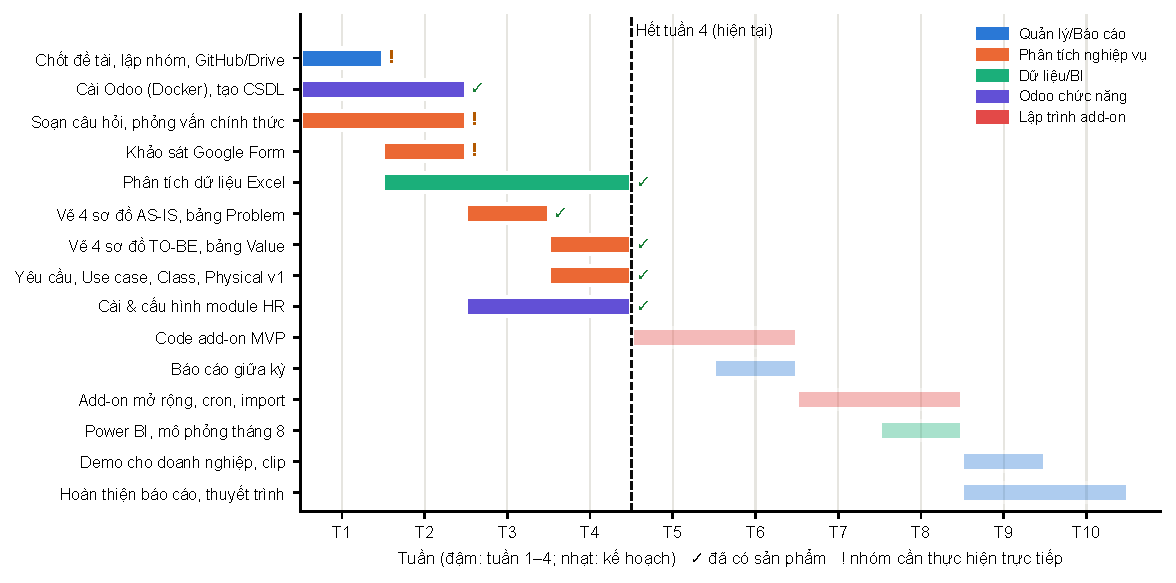
\includegraphics[width=\linewidth]{gantt.pdf}
\caption{Kế hoạch 10 tuần và tiến độ đến hết tuần 4}\label{fig:gantt}
\end{figure}

\begin{table}[H]\centering\small
\caption{Phân công nhiệm vụ}\label{tab:phancong}
\begin{tabularx}{\linewidth}{L{3.3cm}YY}
\toprule \textbf{Vai trò} & \textbf{Phụ trách chính} & \textbf{Hỗ trợ} \\\midrule
TV1 – Nhóm trưởng / BA & Liên hệ doanh nghiệp, phỏng vấn, Chương 1, 3; phiếu xác nhận; tổng hợp báo cáo & Bảng vấn đề, bảng giá trị \\
TV2 – BA / BPMN & 8 sơ đồ BPMN, phân tích nghiệp vụ, use case và đặc tả & Kịch bản demo \\
TV3 – Dữ liệu / BI & Phân tích Excel, mô phỏng tháng 8, Power BI & Dữ liệu demo \\
TV4 – Odoo chức năng & Cài Docker, cấu hình Employees, Recruitment, Website, eLearning, Attendances, Time Off & Triển khai máy chủ \\
TV5 – Lập trình add-on & Add-on \texttt{tpc\_labour\_planning}, thiết kế logic/vật lý & Cron, báo cáo PDF \\
\bottomrule
\end{tabularx}
\end{table}

\section{Kết quả đạt được trong tuần 1–4}
\begin{table}[H]\centering\small
\caption{Đối chiếu đầu ra tuần 1–4 với kế hoạch}\label{tab:tiendo}
\begin{tabularx}{\linewidth}{C{1cm}YL{3.2cm}L{2.6cm}}
\toprule \textbf{Tuần} & \textbf{Đầu ra theo kế hoạch} & \textbf{Kết quả / vị trí} & \textbf{Trạng thái} \\\midrule
1 & Chốt đề tài, lập nhóm, GitHub/Drive & Mục 1.1–1.7 & \textcolor{warn}{Nhóm xác nhận} \\
1 & Cài Odoo bằng Docker, tạo CSDL & Mục 5.1–5.2 & \textcolor{okgreen}{Hoàn thành} \\
1–2 & Bộ câu hỏi phỏng vấn chính thức & Phụ lục A & \textcolor{okgreen}{Đã soạn} \\
2 & Phỏng vấn chính thức, ghi âm, biên bản & Mẫu ở Phụ lục C & \textcolor{warn}{Nhóm thực hiện} \\
2 & Khảo sát Google Form & Phụ lục B & \textcolor{warn}{Đã soạn, chưa gửi} \\
2–4 & Phân tích dữ liệu Excel & Mục 3.4, 4.2 & \textcolor{okgreen}{Hoàn thành} \\
3 & 4 sơ đồ AS-IS, bảng vấn đề & Mục 4.3–4.4 & \textcolor{okgreen}{Bản v1} \\
3–4 & Cài và cấu hình module HR & Mục 5.2–5.3 & \textcolor{okgreen}{Hoàn thành} \\
4 & 4 sơ đồ TO-BE, bảng giá trị & Mục 4.5–4.6 & \textcolor{okgreen}{Bản v1} \\
4 & Yêu cầu, use case, sơ đồ lớp, thiết kế vật lý & Mục 4.7–4.11 & \textcolor{okgreen}{Bản v1} \\
\bottomrule
\end{tabularx}
\end{table}

\begin{canxacnhan}[Lưu ý trung thực]
Các sơ đồ AS-IS của P1, P2 và phần báo cáo cuối ca của P4 dựa trên buổi phỏng vấn sơ bộ. Riêng cách \emph{xếp ca} (P3) và cách \emph{ghi giờ công thực tế} (P4) chưa được hỏi trực tiếp, nên hiện là \textbf{giả định suy ra từ dữ liệu} và được đánh dấu ``cần xác nhận''. Các bước này phải được kiểm chứng ở buổi phỏng vấn chính thức (câu 10–14, Phụ lục A) trước khi chốt bản v2.
\end{canxacnhan}

% =====================================================================
\chapter{Cơ sở lý thuyết}
% =====================================================================

\section{Hệ thống thông tin quản lý và ERP}
Hệ thống thông tin quản lý (HTTTQL) là tập hợp con người, quy trình, dữ liệu và công nghệ nhằm thu thập, xử lý và cung cấp thông tin phục vụ ra quyết định ở các cấp quản lý \cite{laudon}. ERP là dạng HTTTQL tích hợp, dùng một cơ sở dữ liệu chung cho nhiều phân hệ (bán hàng, kho, tài chính, nhân sự), giúp dữ liệu nhập một lần và dùng ở nhiều nơi. Với chuỗi nhà hàng, giá trị của ERP nằm ở chỗ chuẩn hoá quy trình giữa các cửa hàng và đưa số liệu vận hành lên cấp khu vực gần như tức thời.

\section{Quản trị nhân sự, HRIS và xếp ca}
Quản trị nhân sự bao gồm hoạch định, tuyển dụng, đào tạo, đánh giá, đãi ngộ và giữ chân nhân viên \cite{dessler}. Hệ thống thông tin nhân sự (HRIS) số hoá các hoạt động này: hồ sơ nhân viên, ứng viên, đào tạo, chấm công, nghỉ phép.

Bài toán \textbf{xếp ca} (staff scheduling and rostering) gồm các bước: (1) dự báo nhu cầu, (2) chuyển nhu cầu thành số giờ/số người cần theo khung giờ, (3) thiết kế ca, (4) gán nhân viên vào ca theo kỹ năng, giờ tối đa và nguyện vọng \cite{ernst}. Trong ngành bán lẻ, ăn uống, nhu cầu thường được tính từ doanh thu dự báo chia cho năng suất mục tiêu, có ràng buộc số người tối thiểu cho mỗi vị trí. Đây cũng là cách TPC đang tính ``Forecast WH'' trong file Excel: định mức giờ $\approx$ doanh thu dự báo $\div$ 330.000 đ/giờ.

\section{Mô hình hoá quy trình bằng BPMN 2.0}
BPMN (Business Process Model and Notation) là chuẩn ký hiệu của OMG dùng để mô tả trực quan một quy trình từ điểm bắt đầu đến điểm kết thúc, giúp chỉ ra điểm kém hiệu quả và thiết kế quy trình tốt hơn \cite{bpmn,dumas}. Theo tài liệu môn học, BPMN gồm 6 nhóm thành phần chính:
\begin{itemize}
\item \textbf{Swimlane} (Pool, Lane): thể hiện ai làm việc gì. Pool là một thành phần tham gia; Lane là vai trò bên trong pool. Bên ngoài doanh nghiệp (như ứng viên) được vẽ thành pool ``hộp đen''.
\item \textbf{Activity}: Task và Sub-Process. Loại task: User (làm trên hệ thống), Manual (làm tay ngoài hệ thống), Service (hệ thống tự động), Send/Receive, Business Rule. Marker: Loop, Multi-instance, Sub-process.
\item \textbf{Gateway}: Exclusive (XOR), Inclusive (OR), Parallel (AND), Event-based.
\item \textbf{Event}: Start, Intermediate, End; loại thường dùng là Message và Timer.
\item \textbf{Flow}: Sequence flow (trong một pool), Message flow (giữa các pool), Association.
\item \textbf{Information Artifact}: Data Object, Data Object Collection, Data Input/Output, Data Store, Text Annotation.
\end{itemize}
Các lưu ý được áp dụng khi vẽ: xác định rõ điểm bắt đầu và kết thúc; vẽ AS-IS trước để làm nổi bật điểm kém hiệu quả rồi mới vẽ TO-BE; mỗi sơ đồ nằm trên một trang; bố trí sequence flow theo chiều ngang. Hình~\ref{fig:legend} là bảng ký hiệu dùng trong báo cáo; nhóm bổ sung màu nền để người đọc nhận ra nhanh bước gây tắc nghẽn (AS-IS) và bước do hệ thống thực hiện (TO-BE). Màu chỉ để hỗ trợ đọc, không thay đổi ngữ nghĩa BPMN.

\begin{figure}[H]\centering
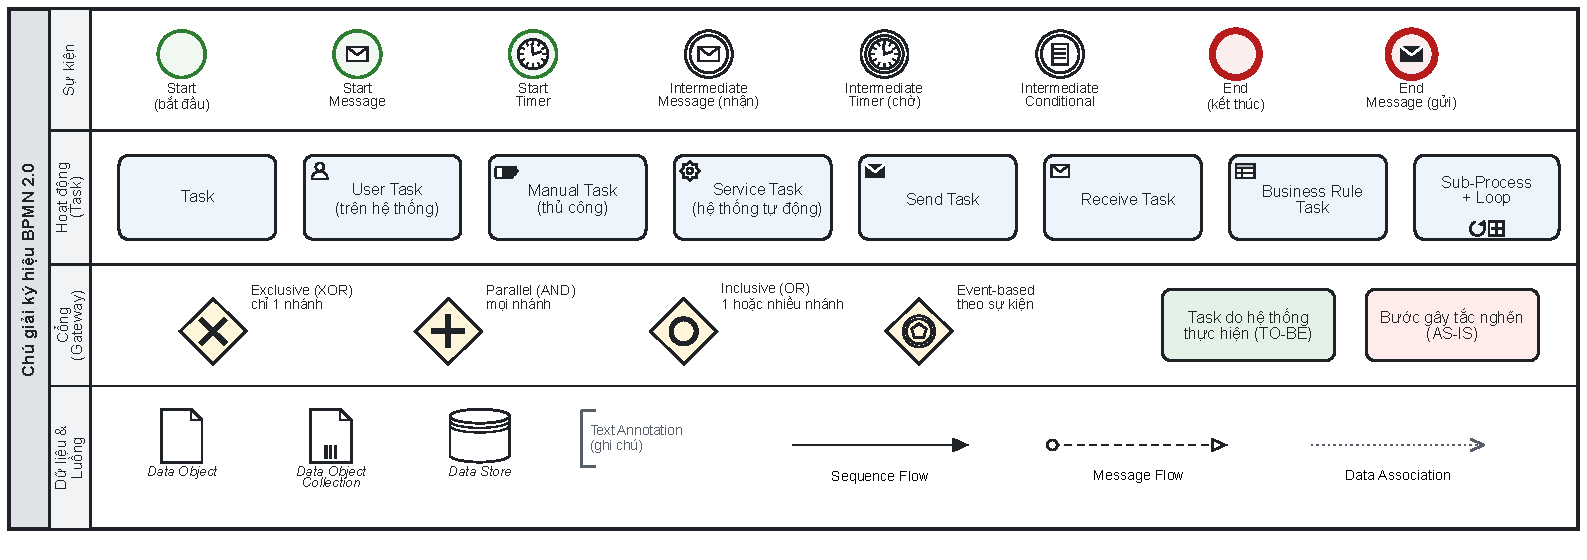
\includegraphics[width=\linewidth]{bpmn_legend.pdf}
\caption{Ký hiệu BPMN 2.0 sử dụng trong báo cáo}\label{fig:legend}
\end{figure}

\section{Nền tảng Odoo}
Odoo là bộ ứng dụng ERP mã nguồn mở viết bằng Python, dùng PostgreSQL. Kiến trúc gồm 3 lớp: giao diện web (OWL/JavaScript), máy chủ ứng dụng (ORM, logic nghiệp vụ) và cơ sở dữ liệu \cite{odoo}. Mỗi chức năng là một \emph{module} gồm \texttt{\_\_manifest\_\_.py}, các model (lớp Python kế thừa \texttt{models.Model}), view (XML), quyền (\texttt{ir.model.access.csv}, record rule) và dữ liệu. Nhờ cơ chế kế thừa (\texttt{\_inherit}), module tự viết có thể thêm field, thêm logic vào model có sẵn như \texttt{hr.employee} mà không sửa mã gốc.

Odoo có 2 phiên bản: \textbf{Community} (miễn phí, tự cài đặt) và \textbf{Enterprise} (trả phí, có thêm Planning, Approvals, Studio, Appraisals...). Bản \textbf{Odoo Online} (SaaS) không cho cài module tự viết. Vì học phần yêu cầu \emph{add-on module}, nhóm chọn \textbf{Odoo 18 Community tự cài đặt bằng Docker}, và tự xây chức năng xếp ca trong add-on thay cho module Planning (Enterprise).

\section{Các chỉ số đo lường}
\begin{table}[H]\centering\small
\caption{Các KPI dùng xuyên suốt đồ án}\label{tab:kpi}
\begin{tabularx}{\linewidth}{L{2.4cm}L{6.4cm}Y}
\toprule \textbf{Chỉ số} & \textbf{Công thức} & \textbf{Ý nghĩa / mục tiêu} \\\midrule
\%COL & $\dfrac{\text{Giờ công thực tế}\times\text{lương TB/giờ}}{\text{Doanh thu}}$ & Mục tiêu công ty: 13,65\% \\
Productivity & Doanh thu / giờ công thực tế & Mục tiêu: 330.000 đ/giờ \\
Giờ công đề xuất & $\max\left(\dfrac{\text{Doanh thu dự báo}}{\text{Productivity mục tiêu}},\ \text{giờ tối thiểu}\right)$ & Cơ sở xếp ca TO-BE \\
Time-to-hire & Số ngày từ lúc ứng viên nộp hồ sơ đến ca làm đầu tiên & Đo hiệu quả tuyển dụng \\
Tỷ lệ hoàn thành đào tạo & Số NV đạt quầy đúng hạn / số NV mới & Đo hiệu quả đào tạo \\
Tỷ lệ nghỉ việc & Số NV nghỉ trong tháng / số NV bình quân & Dự báo nhu cầu tuyển \\
\bottomrule
\end{tabularx}
\end{table}

% =====================================================================
\chapter{Tổng quan doanh nghiệp}
% =====================================================================

\section{Giới thiệu The Pizza Company}
The Pizza Company là chuỗi nhà hàng pizza hoạt động tại nhiều tỉnh thành ở Việt Nam, vận hành theo mô hình cửa hàng do công ty quản lý trực tiếp, chia theo khu vực. Theo quản lý khu vực, công ty có kho tổng riêng nhập hàng từ nhà cung cấp trong nước và nước ngoài, dùng phần mềm SAP cho hàng hoá và phần mềm POS cho bán hàng; công ty vừa chuyển sang website mới trong thời gian phỏng vấn. Mọi thay đổi phần mềm, quy trình đều phải thống nhất giữa các phòng ban, nên đề tài định vị là \emph{nguyên mẫu (prototype)} để doanh nghiệp tham khảo, không thay thế hệ thống đang chạy.

\section{Cơ cấu nhân sự cấp cửa hàng}
\begin{itemize}
\item \textbf{Quản lý cửa hàng (RGM)} và các \textbf{quản lý ca (Shift Manager)}: điều hành ca, xếp ca, tuyển dụng tại chỗ, làm báo cáo cuối ca.
\item \textbf{Nhân viên} khoảng 40–50 người/cửa hàng, phần lớn part-time, chia theo khu vực: phục vụ, thu ngân, bếp (4–5 quầy: make line, cut \& pack...), giao hàng.
\item \textbf{Phòng Nhân sự – Tuyển dụng} (văn phòng): đăng tin, cung cấp data ứng viên khi cửa hàng cần, nhận hồ sơ và cấp mã nhân viên.
\item \textbf{Quản lý khu vực}: giám sát nhiều cửa hàng, nhận báo cáo doanh thu, tài chính hằng ngày qua email.
\end{itemize}

\section{Chỉ tiêu được giao cho cửa hàng}
Theo phỏng vấn và file dữ liệu, cửa hàng được đánh giá theo: doanh thu so với mục tiêu (BP target), số khiếu nại khách hàng, điểm audit vận hành ($\geq$ 90\%), \textbf{\%COL mục tiêu 13,65\%} và \textbf{Productivity mục tiêu 330.000 đ/giờ}. Hai chỉ tiêu cuối gắn trực tiếp với xếp ca nên là KPI trung tâm của đề tài.

\section{Tình hình kinh doanh qua dữ liệu}
Năm 2025, cửa hàng mẫu đạt doanh thu thuần \textbf{17,08 tỷ đồng}. Doanh thu có tính mùa vụ rõ: cao vào tháng 12 và tháng 1 (lễ, Tết), thấp vào tháng 2 và tháng 9 (Hình~\ref{fig:c1}). Quan trọng hơn, doanh thu chênh lệch rất lớn giữa các ngày trong tuần: thứ Hai, thứ Năm, thứ Sáu chỉ bằng khoảng một nửa thứ Bảy, Chủ nhật (Hình~\ref{fig:c2}). Quy luật này lặp lại ổn định, nên hoàn toàn có thể dùng để dự báo và xếp ca.

\begin{figure}[H]\centering
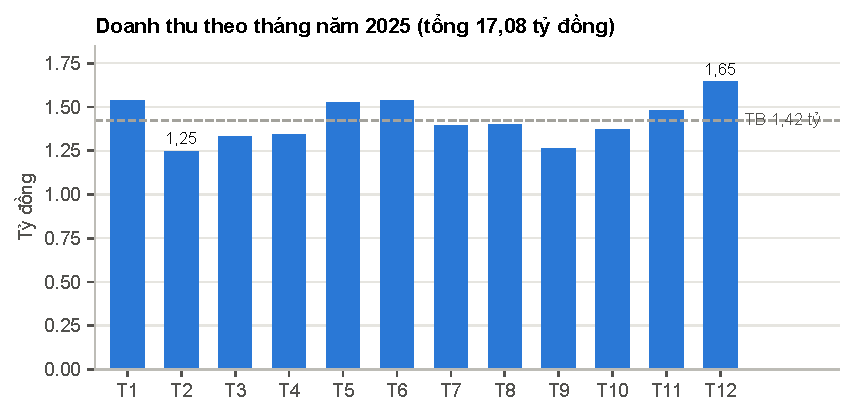
\includegraphics[width=0.92\linewidth]{c1_sales_month_2025.pdf}
\caption{Doanh thu theo tháng năm 2025 (nguồn: sheet \texttt{Sales data})}\label{fig:c1}
\end{figure}
\begin{figure}[H]\centering
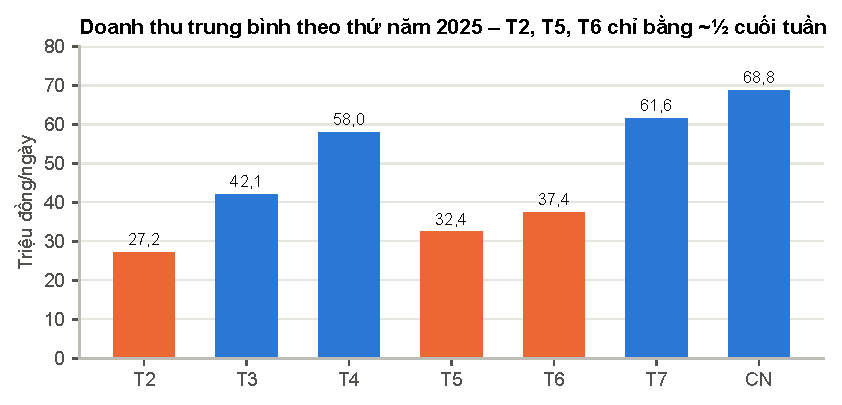
\includegraphics[width=0.92\linewidth]{c2_sales_dow_2025.pdf}
\caption{Doanh thu trung bình theo thứ năm 2025 (nguồn: sheet \texttt{Sales data})}\label{fig:c2}
\end{figure}

Về kênh bán, khách ăn tại chỗ chiếm 41,3\%, các ứng dụng giao đồ ăn (aggregator) chiếm 26,6\% (Hình~\ref{fig:c7}). Hai kênh này cần nhân sự khác nhau (phục vụ tại bàn so với bếp và đóng gói), nên giờ công không chỉ cần đúng \emph{tổng} mà còn cần đúng \emph{quầy}.

\begin{figure}[H]\centering
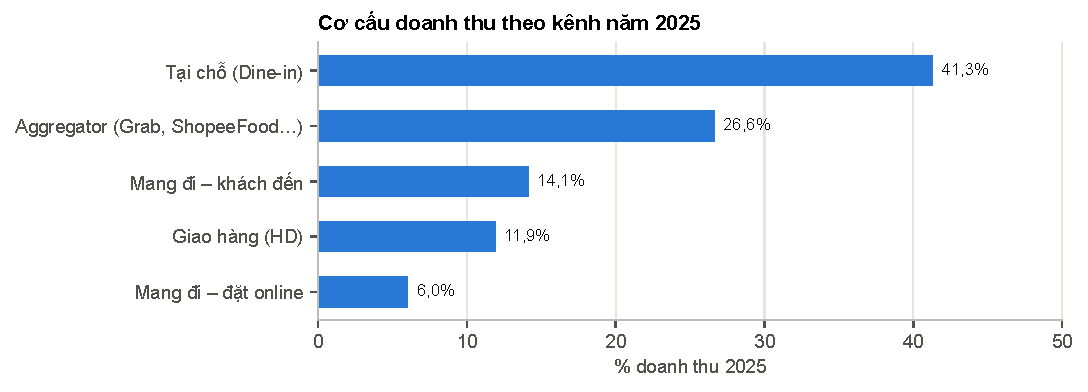
\includegraphics[width=0.86\linewidth]{c7_channel_2025.pdf}
\caption{Cơ cấu doanh thu theo kênh năm 2025}\label{fig:c7}
\end{figure}

% =====================================================================
\chapter{Phân tích nghiệp vụ và thiết kế hệ thống}
% =====================================================================

\section{Thu thập yêu cầu}
\subsection{Phỏng vấn sơ bộ}
Buổi phỏng vấn sơ bộ với quản lý khu vực (2 thành viên nhóm tham gia, có bản gỡ băng) cho các phát hiện chính ở Bảng~\ref{tab:phathien}.

\begin{longtable}{L{2.6cm}L{6.6cm}L{5.2cm}}
\caption{Tóm tắt phát hiện từ phỏng vấn sơ bộ}\label{tab:phathien}\\
\toprule \textbf{Chủ đề} & \textbf{Trích ý chính của quản lý} & \textbf{Ý nghĩa cho đề tài} \\\midrule\endfirsthead
\toprule \textbf{Chủ đề} & \textbf{Trích ý chính của quản lý} & \textbf{Ý nghĩa cho đề tài} \\\midrule\endhead
Khó khăn chính & ``Tuyển và đào tạo''; NV part-time gắn bó kém, nghỉ nhiều sau Tết; khu vực ít trường đại học khó tuyển & Chọn mảng HR; cần báo cáo nghỉ việc theo tháng để tuyển trước \\
Quy trình tuyển & Cửa hàng tự tuyển (standee, fanpage) hoặc nhờ phòng TD gửi data; hẹn PV (VD thứ Hai, thứ Năm 10–12h); PV chung rồi mới chọn quầy & Ứng viên đến từ nhiều nguồn rời rạc \\
Thủ tục nhận việc & Điền link + phiếu giấy; cần TK Techcombank; QL mang hồ sơ lên văn phòng; hôm sau có mã NV; ``PV thứ Hai → nộp thứ Ba → có mã thứ Tư → đi làm thứ Năm'' & Time-to-hire 2–4 ngày chỉ vì thủ tục giấy \\
Đào tạo & Có training plan 2 tuần, tài liệu chuẩn theo quầy, có bài test; ``tiến độ đào tạo không đồng đều'' (1 buổi đến 2 tuần) & Cần theo dõi tiến độ từng người, ghi nhận ``đạt quầy'' \\
Báo cáo cuối ca & Khoảng 30 phút; báo cáo doanh thu, tài chính làm Excel gửi email QLKV; có lúc trễ do mất mạng, POS lỗi & \%COL không có sẵn trong ngày \\
Thay đổi hệ thống & Thay đổi phần mềm tốn kém, phải thống nhất nhiều phòng ban & Định vị đề tài là prototype bổ trợ, trao đổi dữ liệu qua file \\
\bottomrule
\end{longtable}

\subsection{Phỏng vấn chính thức và khảo sát}
Bộ 17 câu hỏi cho buổi phỏng vấn chính thức (Phụ lục A) được gửi trước cho quản lý, tập trung vào những điểm buổi sơ bộ chưa làm rõ: cách xếp ca, số người tối thiểu mỗi quầy, cách ghi giờ công, tỷ lệ nghỉ việc theo tháng. Phiếu khảo sát Google Form (Phụ lục B) dành cho 3–5 quản lý ca và nhân viên part-time, nhằm có thêm số liệu định lượng (thời gian xếp ca mỗi tuần, số lần đổi ca, thời gian từ PV đến ca đầu tiên).

\begin{canxacnhan}[Nhóm cần thực hiện]
Tổ chức buổi phỏng vấn chính thức (có ghi âm, xin phép trước), gỡ băng thành biên bản theo mẫu Phụ lục C; gửi khảo sát và tổng hợp kết quả. Sau đó cập nhật các bước ``cần xác nhận'' trong sơ đồ AS-IS lên bản v2.
\end{canxacnhan}

\subsection{Dữ liệu thứ cấp}
File \texttt{Data\_do\_an.xlsx} gồm 20 sheet. Nhóm dùng chủ yếu sheet \texttt{Sales data} (doanh thu theo ngày năm 2025; năm 2026 có thêm Forecast Sales, Forecast WH, Actual WH, \%COL, Productivity) và \texttt{Store Perfomance} (bảng theo dõi tháng 8/2026). Các sheet có thông tin cá nhân (tên nhân viên, số điện thoại khách, ngày sinh của trẻ em) \textbf{không được đưa vào báo cáo hay Odoo demo}; dữ liệu nhân viên trong Odoo đều là tên giả.

\section{Phân tích dữ liệu hiện trạng nhân công}
\subsection{Giờ công và \%COL theo tháng}
Trong 8 tháng đầu năm 2026, giờ công thực tế vượt định mức ở 7/8 tháng (Hình~\ref{fig:c3}); tháng 2 vượt nhiều nhất (+1.601 giờ) do kỳ nghỉ Tết. \%COL vượt mục tiêu 13,65\% ở 6/8 tháng, trong khi nếu xếp đúng định mức thì cả 8 tháng đều dưới mục tiêu (Hình~\ref{fig:c4}). Nói cách khác, \textbf{định mức hiện tại là khả thi; khoảng cách nằm ở khâu xếp ca}.

\begin{figure}[H]\centering
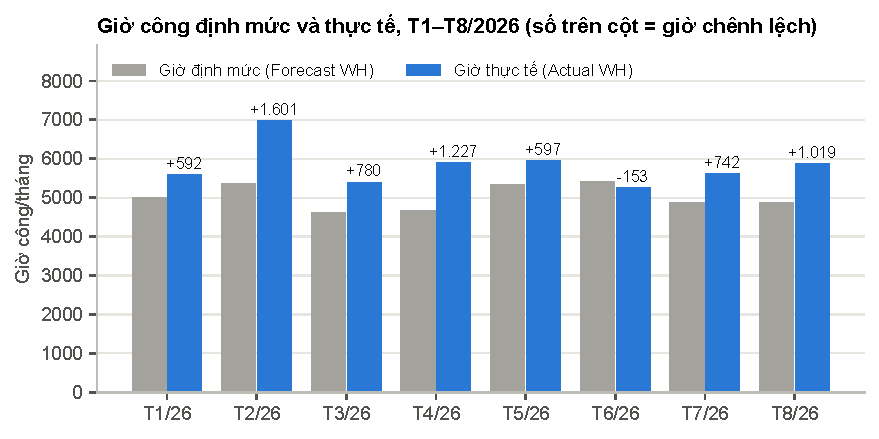
\includegraphics[width=0.92\linewidth]{c3_hours_month_2026.pdf}
\caption{Giờ công định mức và thực tế theo tháng, T1–T8/2026}\label{fig:c3}
\end{figure}
\begin{figure}[H]\centering
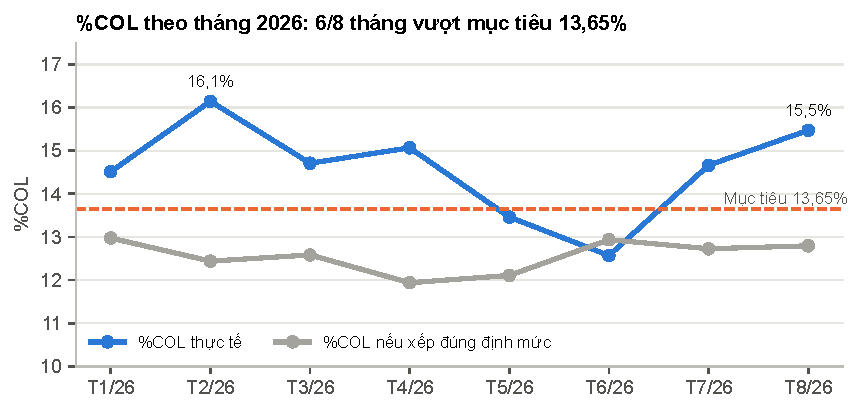
\includegraphics[width=0.92\linewidth]{c4_col_month_2026.pdf}
\caption{\%COL theo tháng so với mục tiêu, T1–T8/2026}\label{fig:c4}
\end{figure}

\subsection{Giờ công theo thứ trong tuần}
Bảng~\ref{tab:thu8} và Hình~\ref{fig:c5} cho thấy cùng một mẫu hình: ngày vắng (thứ Hai, Năm, Sáu) dùng nhiều giờ hơn định mức 50–70 giờ/ngày, \%COL lên tới 19,8–22\%; ngày đông (thứ Bảy, Chủ nhật) lại thiếu giờ. Loại các ngày lễ/Tết, trong 8 tháng thứ Hai vượt 2.118 giờ, thứ Năm vượt 1.794 giờ, còn Chủ nhật thiếu 1.099 giờ. Đây là dấu hiệu \textbf{xếp ca theo khung cố định mỗi ngày}, chưa co giãn theo doanh thu.

\begin{table}[H]\centering\small
\setlength{\tabcolsep}{4pt}\caption{Bình quân một ngày theo thứ, tháng 8/2026 (nguồn: \texttt{Store Perfomance}, \texttt{Sales data})}\label{tab:thu8}
\begin{tabular}{lrrrrr}
\toprule \textbf{Thứ} & \textbf{Doanh thu (nghìn đ)} & \textbf{Giờ thực tế} & \textbf{Giờ định mức} & \textbf{Chênh lệch} & \textbf{\%COL} \\\midrule
Thứ Hai & 33.588 & 165,1 & 93,5 & +71,6 & \textbf{19,8\%} \\
Thứ Ba & 51.707 & 205,6 & 168,5 & +37,1 & 16,0\% \\
Thứ Tư & 65.802 & 218,1 & 208,1 & +10,0 & 13,3\% \\
Thứ Năm & 31.373 & 171,7 & 100,4 & +71,3 & \textbf{22,0\%} \\
Thứ Sáu & 40.697 & 164,9 & 115,0 & +49,9 & 16,3\% \\
Thứ Bảy & 56.830 & 198,4 & 195,4 & +3,0 & 14,1\% \\
Chủ nhật & 63.952 & 204,6 & 210,3 & $-$5,7 & 12,9\% \\
\midrule
\textbf{Cả tháng} & \textbf{1.530.168} & \textbf{5.882} & \textbf{4.863} & \textbf{+1.018} & \textbf{15,5\%} \\
\bottomrule
\end{tabular}
\end{table}

\begin{figure}[H]\centering
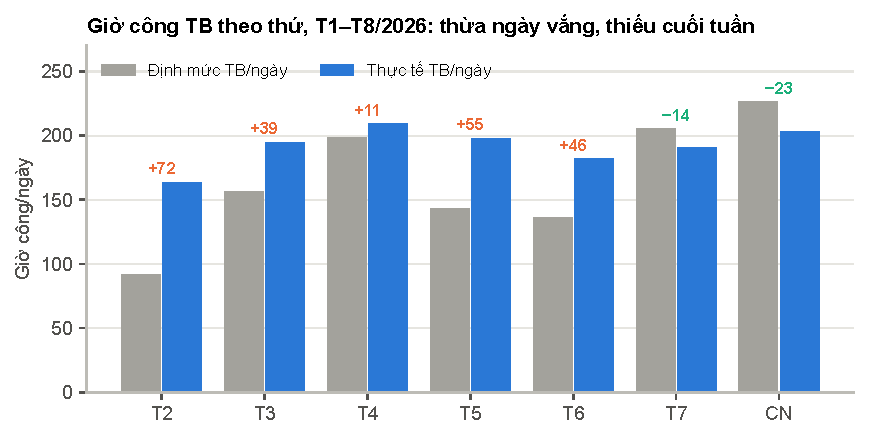
\includegraphics[width=0.92\linewidth]{c5_hours_dow_2026.pdf}
\caption{Giờ công bình quân theo thứ, T1–T8/2026}\label{fig:c5}
\end{figure}

\subsection{Mối quan hệ giữa doanh thu và giờ công}
Nếu xếp ca theo năng suất mục tiêu, giờ công phải tăng gần tỷ lệ với doanh thu (đường cam ở Hình~\ref{fig:c6}). Thực tế, giờ công ngày thường dao động trong một dải hẹp 130–230 giờ bất kể doanh thu 20 hay 90 triệu đồng: hệ số tương quan giữa doanh thu và giờ thực tế chỉ 0,66, so với 0,86 của giờ định mức. Ngày doanh thu thấp nằm phía trên đường cam (thừa người), ngày doanh thu cao nằm phía dưới (thiếu người, ảnh hưởng chất lượng phục vụ).

\begin{figure}[H]\centering
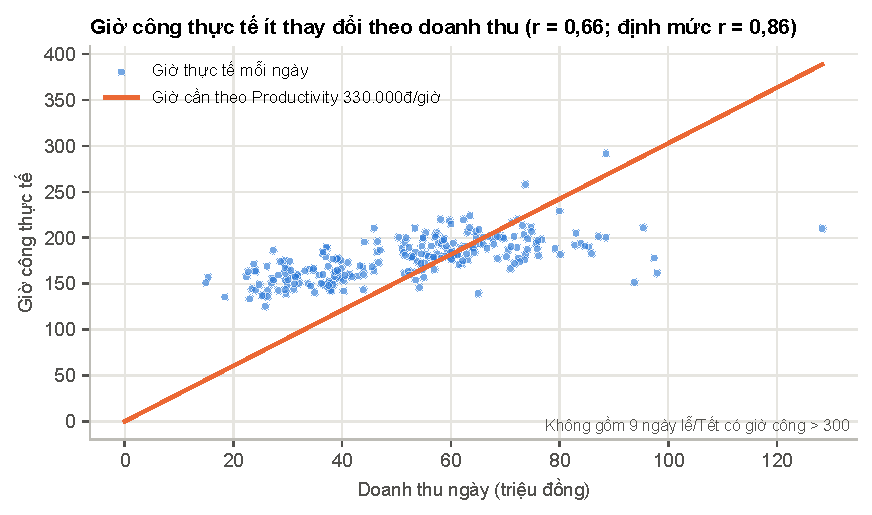
\includegraphics[width=0.92\linewidth]{c6_scatter_2026.pdf}
\caption{Doanh thu ngày và giờ công thực tế, T1–T8/2026 (không gồm 9 ngày lễ/Tết)}\label{fig:c6}
\end{figure}

\begin{canxacnhan}[Cần xác nhận với doanh nghiệp]
(1) 9 ngày lễ/Tết có giờ công 490–640 giờ/ngày: giờ công đã nhân hệ số lương lễ hay là số giờ thật? (2) Mỗi quầy, mỗi khung giờ cần tối thiểu bao nhiêu người? Ràng buộc này quyết định ngày vắng có thể giảm về sát định mức hay không, nên con số tiết kiệm thực tế sẽ chỉ được tính sau khi có câu trả lời và chạy mô phỏng (tuần 8).
\end{canxacnhan}

\section{Phân tích quy trình hiện tại (AS-IS)}
\subsection{Bức tranh tổng thể}
Bốn quy trình nhân sự cấp cửa hàng nối với nhau thành một vòng lặp (Hình~\ref{fig:overview}): tuyển dụng (P1) đưa người vào onboarding và đào tạo (P2); nhân viên đạt quầy được xếp ca hằng tuần (P3); chấm công và theo dõi \%COL (P4) cho biết ca đã xếp hợp lý chưa. Khi thiếu người hoặc có nhân viên nghỉ, vòng lặp quay về P1.

\begin{figure}[H]\centering
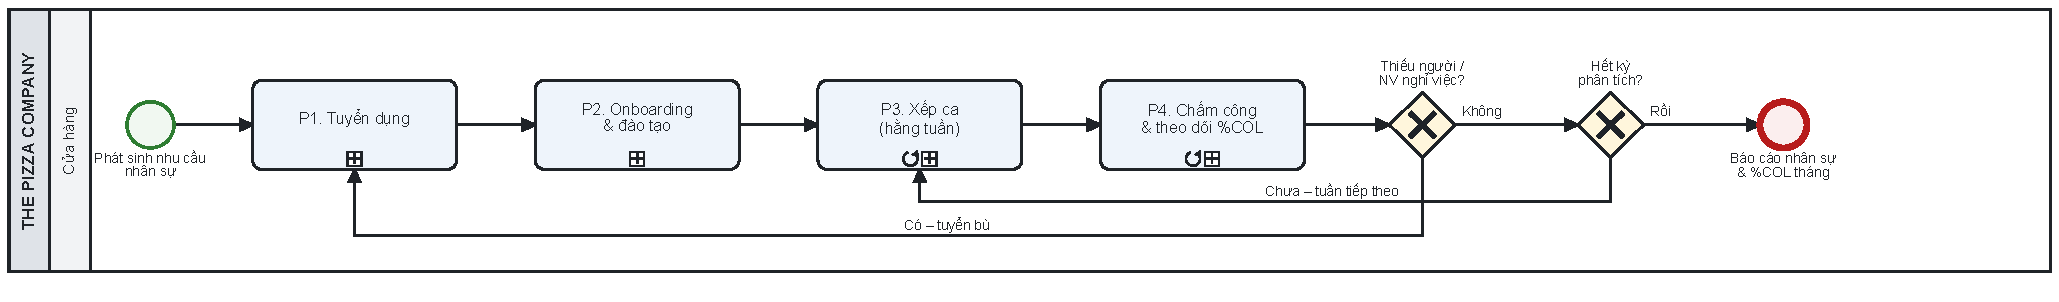
\includegraphics[width=\linewidth]{overview.pdf}
\caption{Chuỗi 4 quy trình nhân sự cấp cửa hàng (mức tổng quát, mỗi bước là một sub-process)}\label{fig:overview}
\end{figure}

% ---------------- P1 AS-IS
\begin{landscape}
\subsection{P1 – Tuyển dụng}
\begin{figure}[H]\centering
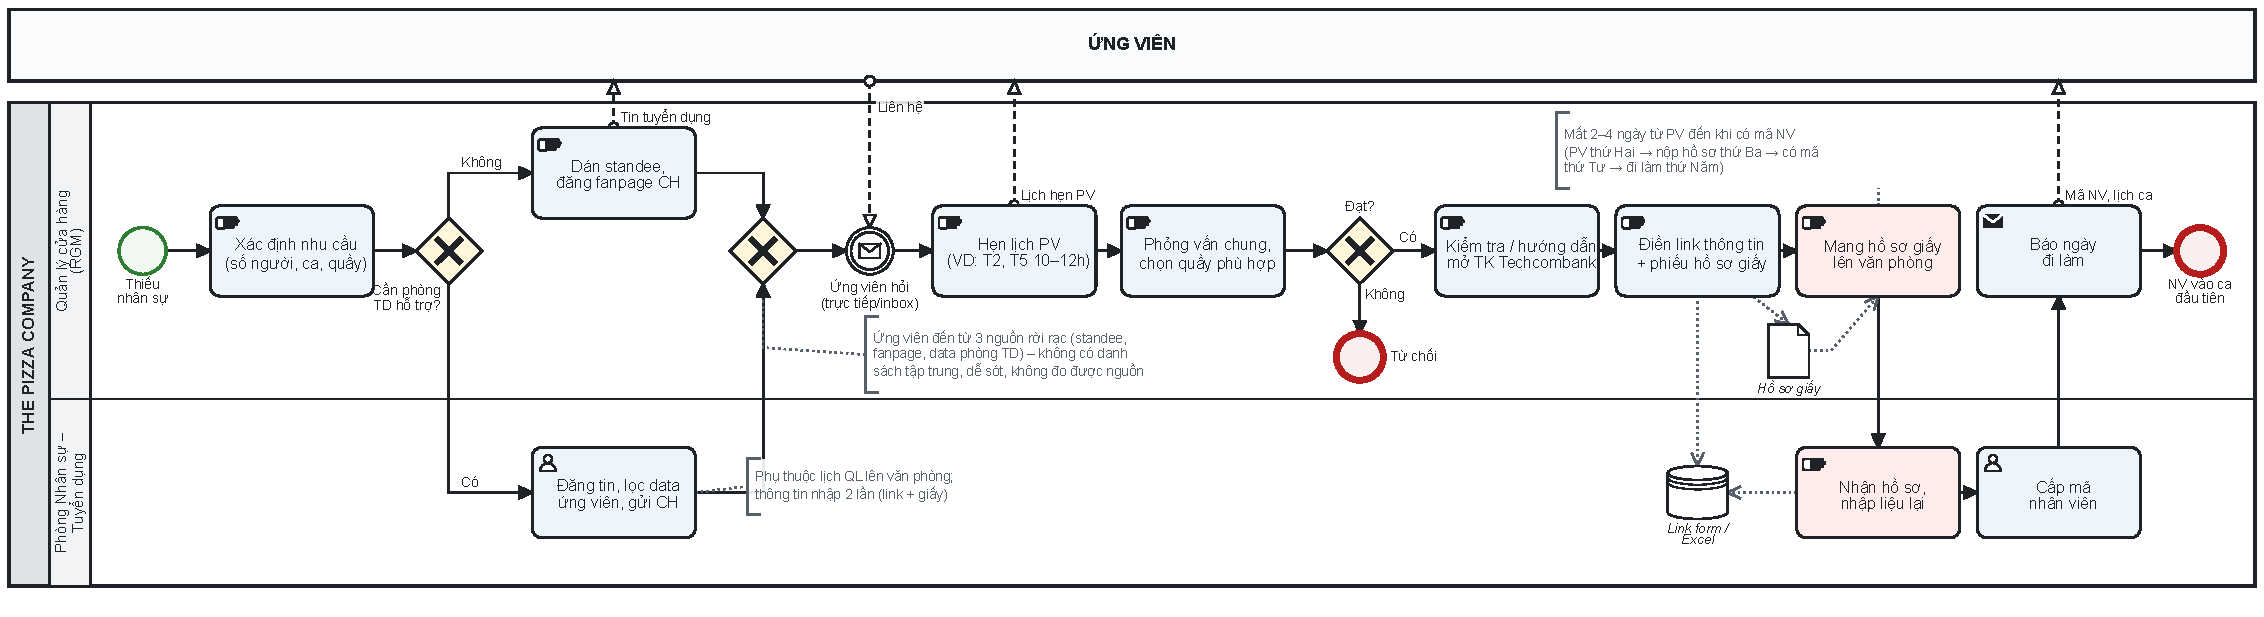
\includegraphics[width=\linewidth]{p1_asis.pdf}
\caption{P1 – Quy trình tuyển dụng hiện tại (AS-IS)}\label{fig:p1asis}
\end{figure}
Khi thiếu nhân sự, quản lý cửa hàng tự quyết định tuyển: dán standee, đăng fanpage cửa hàng, hoặc nhờ phòng Tuyển dụng đăng tin và gửi data ứng viên (Hình~\ref{fig:p1asis}). Ứng viên hỏi trực tiếp tại cửa hàng hoặc nhắn tin; quản lý hẹn lịch phỏng vấn theo khung cố định. Sau phỏng vấn chung, quản lý chọn quầy phù hợp; nếu đạt thì kiểm tra hoặc hướng dẫn mở tài khoản Techcombank (để nhận lương), cho ứng viên điền link thông tin và phiếu hồ sơ giấy. Quản lý mang hồ sơ giấy lên văn phòng theo lịch của mình; phòng Nhân sự nhập liệu lại và cấp mã nhân viên, thường vào hôm sau. \textbf{Điểm nghẽn}: ứng viên phân tán ở 3 nguồn, không có danh sách chung; thông tin nhập 2 lần (link và giấy); thời gian chờ mã NV phụ thuộc lịch quản lý lên văn phòng.
\end{landscape}

% ---------------- P2 AS-IS
\begin{landscape}
\subsection{P2 – Onboarding và đào tạo}
\begin{figure}[H]\centering
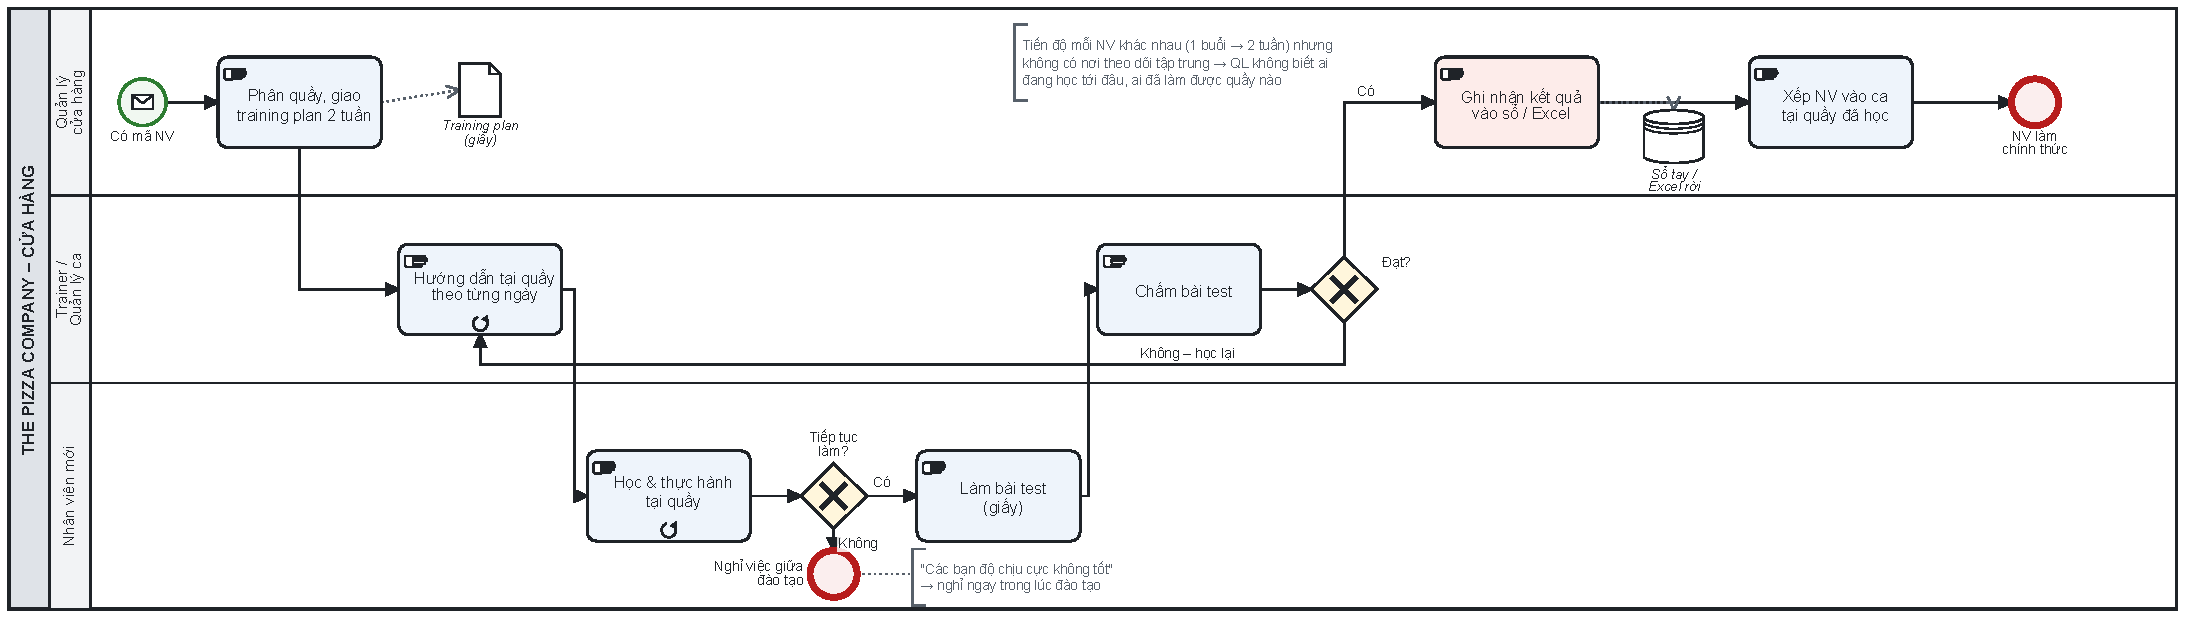
\includegraphics[width=\linewidth]{p2_asis.pdf}
\caption{P2 – Quy trình onboarding và đào tạo hiện tại (AS-IS)}\label{fig:p2asis}
\end{figure}
Khi có mã nhân viên, quản lý phân quầy và giao training plan 2 tuần (Hình~\ref{fig:p2asis}). Trainer hoặc quản lý ca hướng dẫn tại quầy theo từng ngày, nhân viên học và thực hành lặp lại; cuối kỳ làm bài test trên giấy, trainer chấm. Không đạt thì học lại; đạt thì quản lý ghi nhận vào sổ hoặc file Excel riêng và xếp nhân viên vào ca. Một tỷ lệ nhân viên nghỉ ngay trong giai đoạn đào tạo vì ``chịu cực không tốt''. \textbf{Điểm nghẽn}: tiến độ mỗi người khác nhau nhưng không có nơi theo dõi tập trung, nên quản lý không biết ngay ai đã làm được quầy nào để xếp ca.
\end{landscape}

% ---------------- P3 AS-IS
\begin{landscape}
\subsection{P3 – Xếp ca \textnormal{\small(giả định, cần xác nhận)}}
\begin{figure}[H]\centering
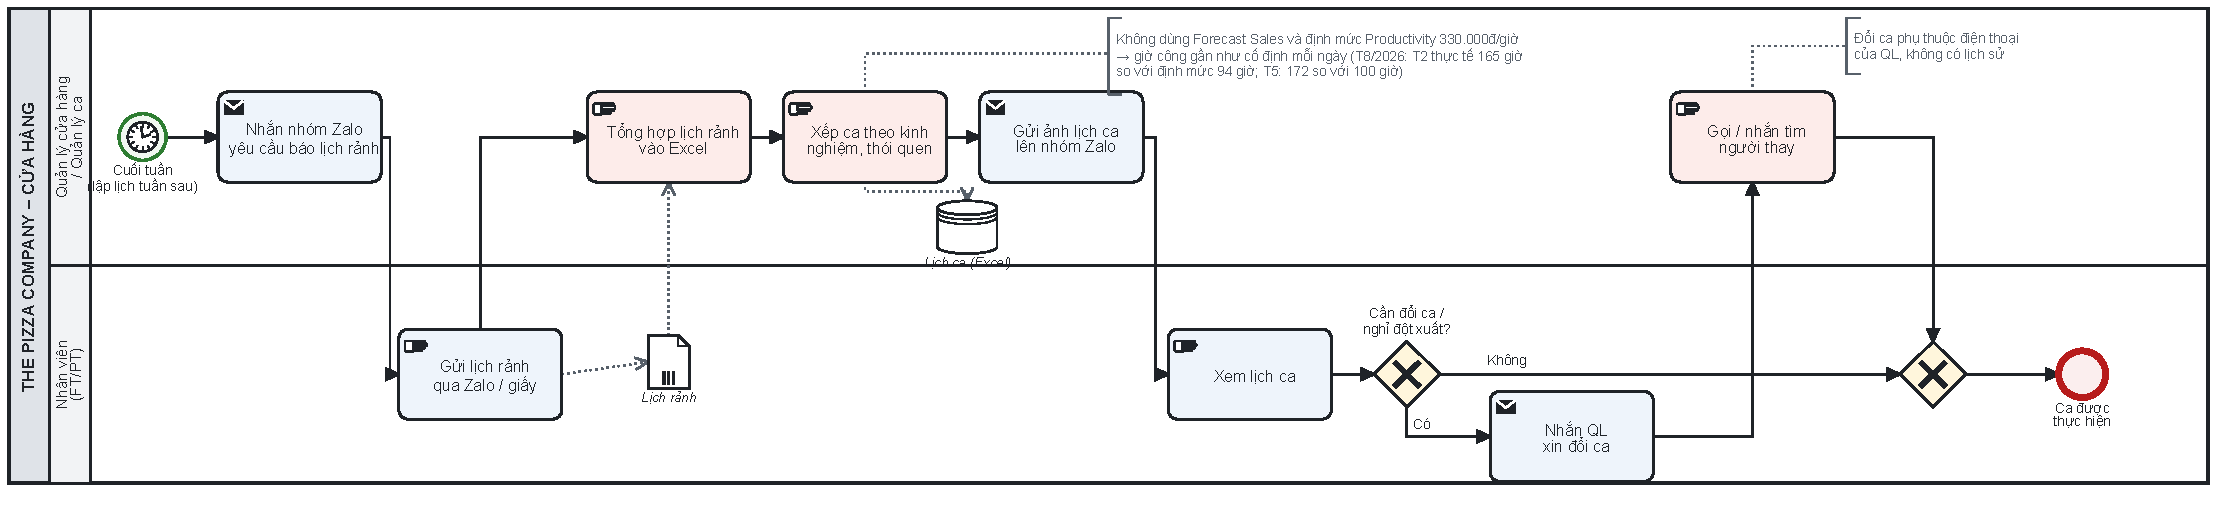
\includegraphics[width=\linewidth]{p3_asis.pdf}
\caption{P3 – Quy trình xếp ca hiện tại (AS-IS, giả định suy ra từ dữ liệu – cần xác nhận)}\label{fig:p3asis}
\end{figure}
Cuối tuần, quản lý nhắn nhóm Zalo yêu cầu nhân viên báo lịch rảnh, tổng hợp vào Excel rồi xếp ca theo kinh nghiệm và gửi ảnh lịch ca lên nhóm (Hình~\ref{fig:p3asis}). Khi nhân viên cần đổi ca hoặc nghỉ đột xuất, quản lý gọi điện, nhắn tin tìm người thay. Dữ liệu ở Mục 4.2 cho thấy giờ công gần như cố định mỗi ngày, nên khả năng cao là việc xếp ca \emph{không dựa trên} Forecast Sales và định mức 330.000 đ/giờ dù hai số này đã có trong file của công ty. \textbf{Điểm nghẽn}: tổng hợp lịch rảnh thủ công; xếp ca không theo dự báo; đổi ca không có lịch sử, không biết người thay có đủ kỹ năng hay không.
\end{landscape}

% ---------------- P4 AS-IS
\begin{landscape}
\subsection{P4 – Chấm công, báo cáo cuối ca và theo dõi \%COL}
\begin{figure}[H]\centering
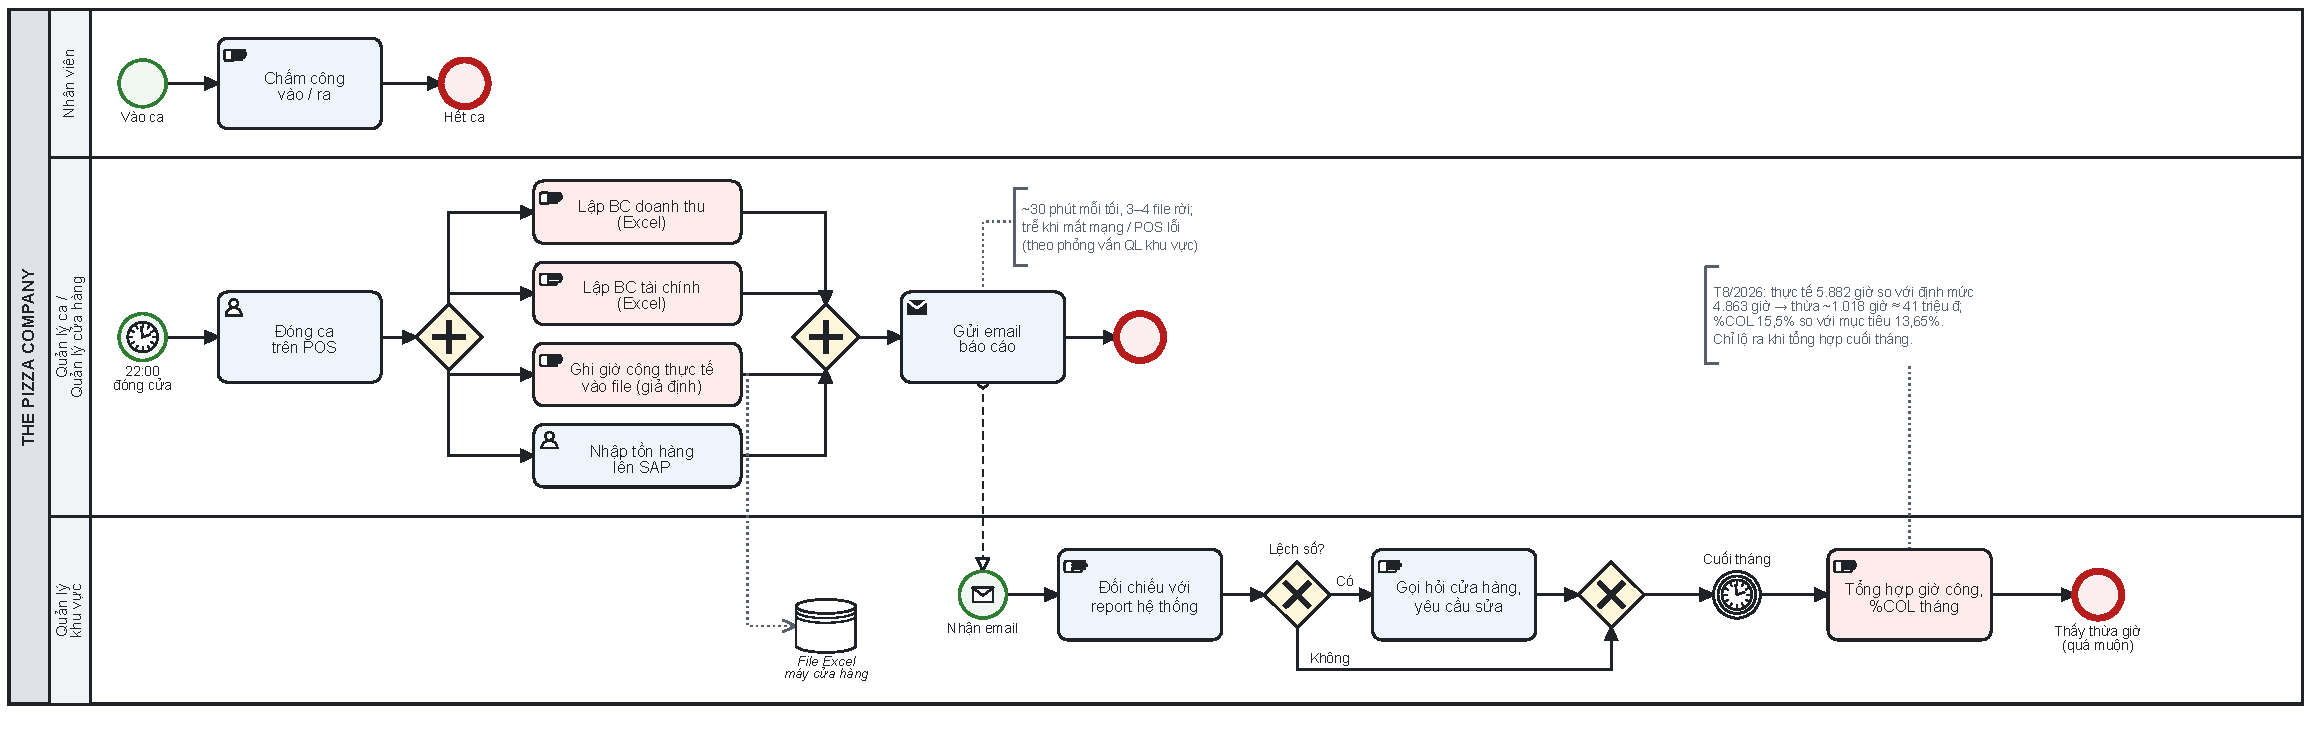
\includegraphics[width=\linewidth]{p4_asis.pdf}
\caption{P4 – Quy trình chấm công, báo cáo cuối ca và theo dõi \%COL hiện tại (AS-IS)}\label{fig:p4asis}
\end{figure}
Nhân viên chấm công vào/ra (Hình~\ref{fig:p4asis}). Khoảng 22:00, quản lý ca đóng ca trên POS rồi song song lập báo cáo doanh thu, báo cáo tài chính trên Excel, ghi giờ công thực tế vào file (giả định, cần xác nhận) và nhập tồn hàng lên SAP; sau đó gửi email cho quản lý khu vực. Quá trình mất khoảng 30 phút mỗi tối và có thể trễ khi mất mạng hoặc POS lỗi. Quản lý khu vực đối chiếu với report hệ thống, nếu lệch thì gọi hỏi cửa hàng. \%COL tháng chỉ được tổng hợp cuối tháng (sheet \texttt{Store Perfomance}). \textbf{Điểm nghẽn}: nhiều file rời; \%COL không có sẵn hằng ngày nên không kịp điều chỉnh ca của ngày hôm sau.
\end{landscape}

\section{Bảng vấn đề (Problem/Issue)}
\begin{longtable}{C{0.7cm}L{3.8cm}C{0.8cm}L{4.0cm}L{4.1cm}}
\caption{Các vấn đề của quy trình hiện tại và bằng chứng}\label{tab:problem}\\
\toprule \textbf{Mã} & \textbf{Vấn đề} & \textbf{QT} & \textbf{Bằng chứng} & \textbf{Ảnh hưởng} \\\midrule\endfirsthead
\toprule \textbf{Mã} & \textbf{Vấn đề} & \textbf{QT} & \textbf{Bằng chứng} & \textbf{Ảnh hưởng} \\\midrule\endhead
I1 & Ứng viên phân tán ở standee, fanpage, data phòng TD; không có danh sách chung & P1 & Phỏng vấn sơ bộ & Dễ sót ứng viên; không đo được nguồn nào hiệu quả \\
I2 & Thủ tục giấy, mang hồ sơ lên văn phòng, nhập liệu 2 lần & P1 & ``PV thứ Hai … đi làm thứ Năm'' & Mất 2–4 ngày; cửa hàng thiếu người trong lúc chờ \\
I3 & Không theo dõi được tiến độ đào tạo từng người & P2 & ``Tiến độ đào tạo không đồng đều'' & Không biết ai làm được quầy nào để xếp ca \\
I4 & Xếp ca theo khung cố định, không theo dự báo doanh thu & P3 & T8/2026 thừa 1.018 giờ; T2, T5 thừa $\sim$71 giờ/ngày; cuối tuần thiếu giờ & Thừa $\approx$ 41 triệu đ/tháng; \%COL 15,5\% so với 13,65\%; thiếu người ngày đông \\
I5 & Đổi ca qua điện thoại, Zalo, không có lịch sử & P3 & Giả định – cần xác nhận (câu 13) & Khó tìm người thay đủ kỹ năng \\
I6 & Báo cáo cuối ca nhiều file Excel, gửi email; \%COL chỉ thấy cuối tháng & P4 & ``Khoảng 30 phút'', ``có trễ''; sheet \texttt{Store Perfomance} nhập tay & Phát hiện thừa giờ muộn, không kịp chỉnh ca \\
I7 & Không dự báo được đợt nghỉ việc (sau Tết) & P1 & Phỏng vấn; T2/2026 giờ công biến động mạnh & Tuyển bù bị động \\
\bottomrule
\end{longtable}

\section{Thiết kế quy trình cải tiến (TO-BE)}
Nguyên tắc thiết kế: (1) dữ liệu nhập một lần tại nguồn; (2) để hệ thống làm việc lặp lại (gửi email, tính toán, nhắc việc); (3) quản lý vẫn là người ra quyết định cuối (duyệt ca, nhận người); (4) giữ cách làm quen thuộc của doanh nghiệp (VD: vẫn nhập Forecast bằng file Excel đúng mẫu đang dùng).

\begin{landscape}
\subsection{P1 – Tuyển dụng trên Odoo Recruitment}
\begin{figure}[H]\centering
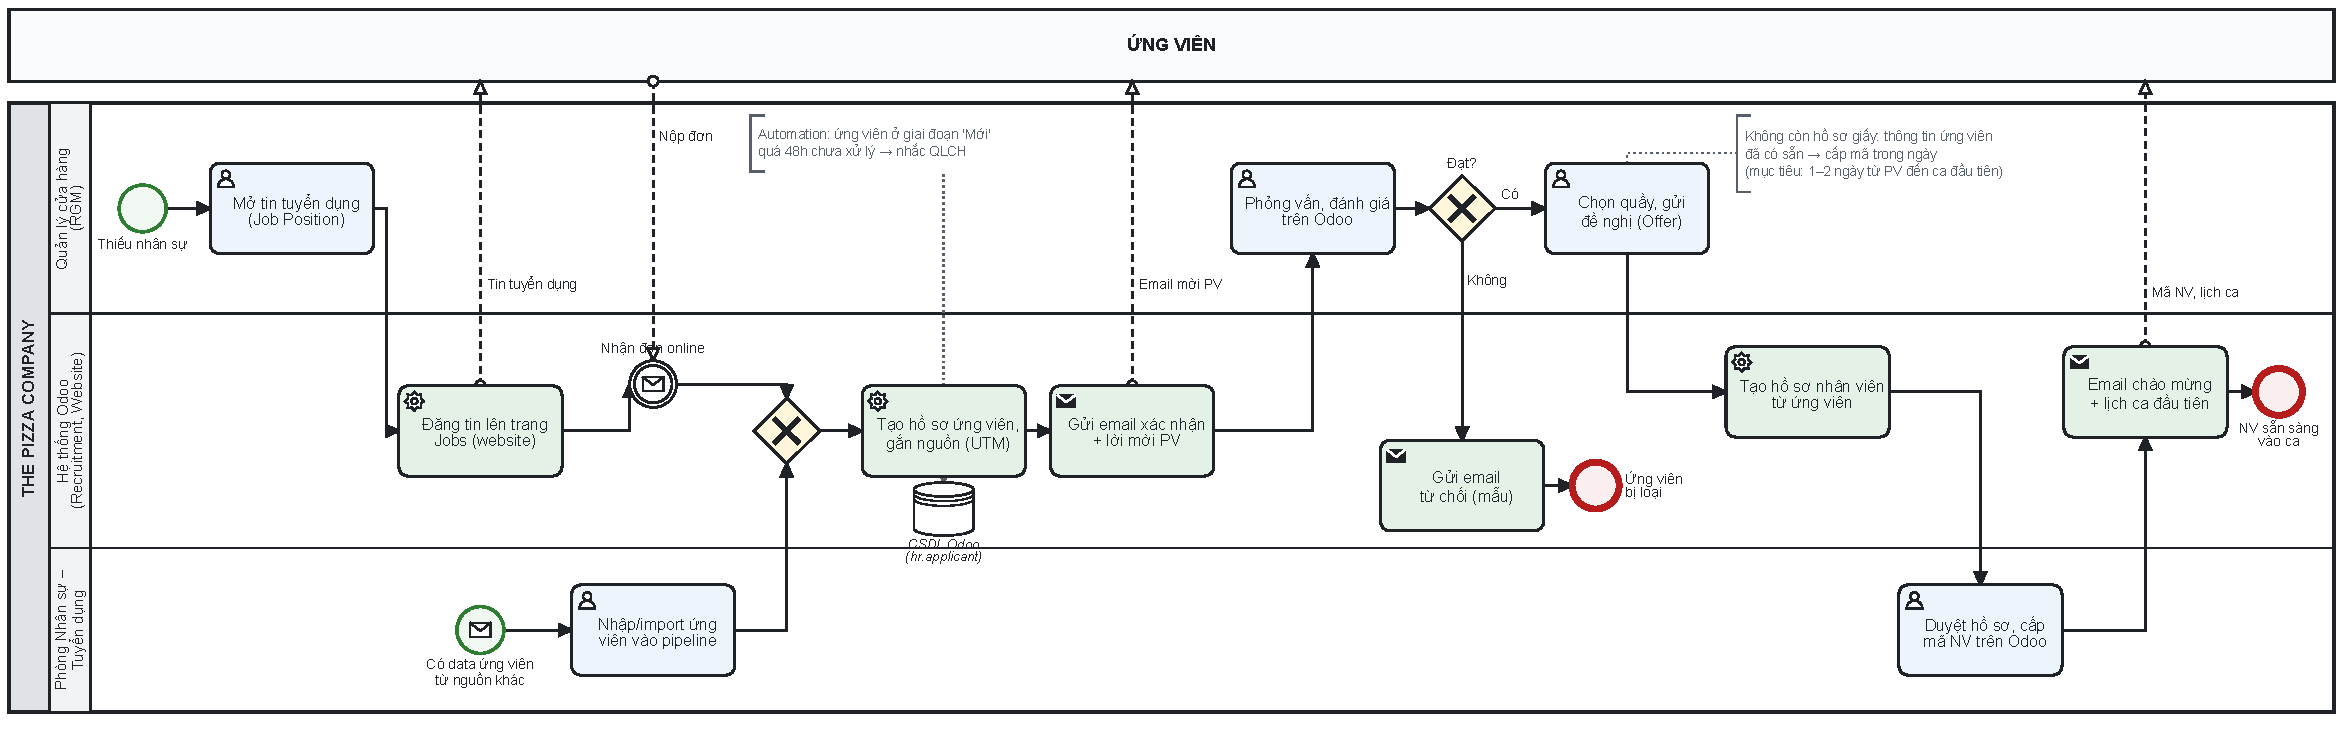
\includegraphics[width=\linewidth]{p1_tobe.pdf}
\caption{P1 – Quy trình tuyển dụng đề xuất trên Odoo (TO-BE)}\label{fig:p1tobe}
\end{figure}
Quản lý mở tin trên Odoo (Job Position); hệ thống đăng tin lên trang Jobs của website (Hình~\ref{fig:p1tobe}). Ứng viên nộp đơn online; ứng viên từ nguồn khác do phòng TD nhập/import vào cùng một pipeline. Hệ thống tạo hồ sơ, gắn nguồn (UTM), gửi email xác nhận và lời mời phỏng vấn. Quản lý phỏng vấn, đánh giá ngay trên Odoo; không đạt thì hệ thống gửi email từ chối theo mẫu; đạt thì quản lý chọn quầy, gửi đề nghị, hệ thống tạo hồ sơ nhân viên từ ứng viên, phòng Nhân sự duyệt và cấp mã trên hệ thống, rồi hệ thống gửi email chào mừng kèm lịch ca đầu tiên. \textbf{Thay đổi chính}: bỏ hồ sơ giấy và bước mang hồ sơ lên văn phòng; mọi ứng viên nằm trong một pipeline có nguồn rõ ràng.
\end{landscape}

\begin{landscape}
\subsection{P2 – Onboarding và đào tạo trên eLearning và Skills}
\begin{figure}[H]\centering
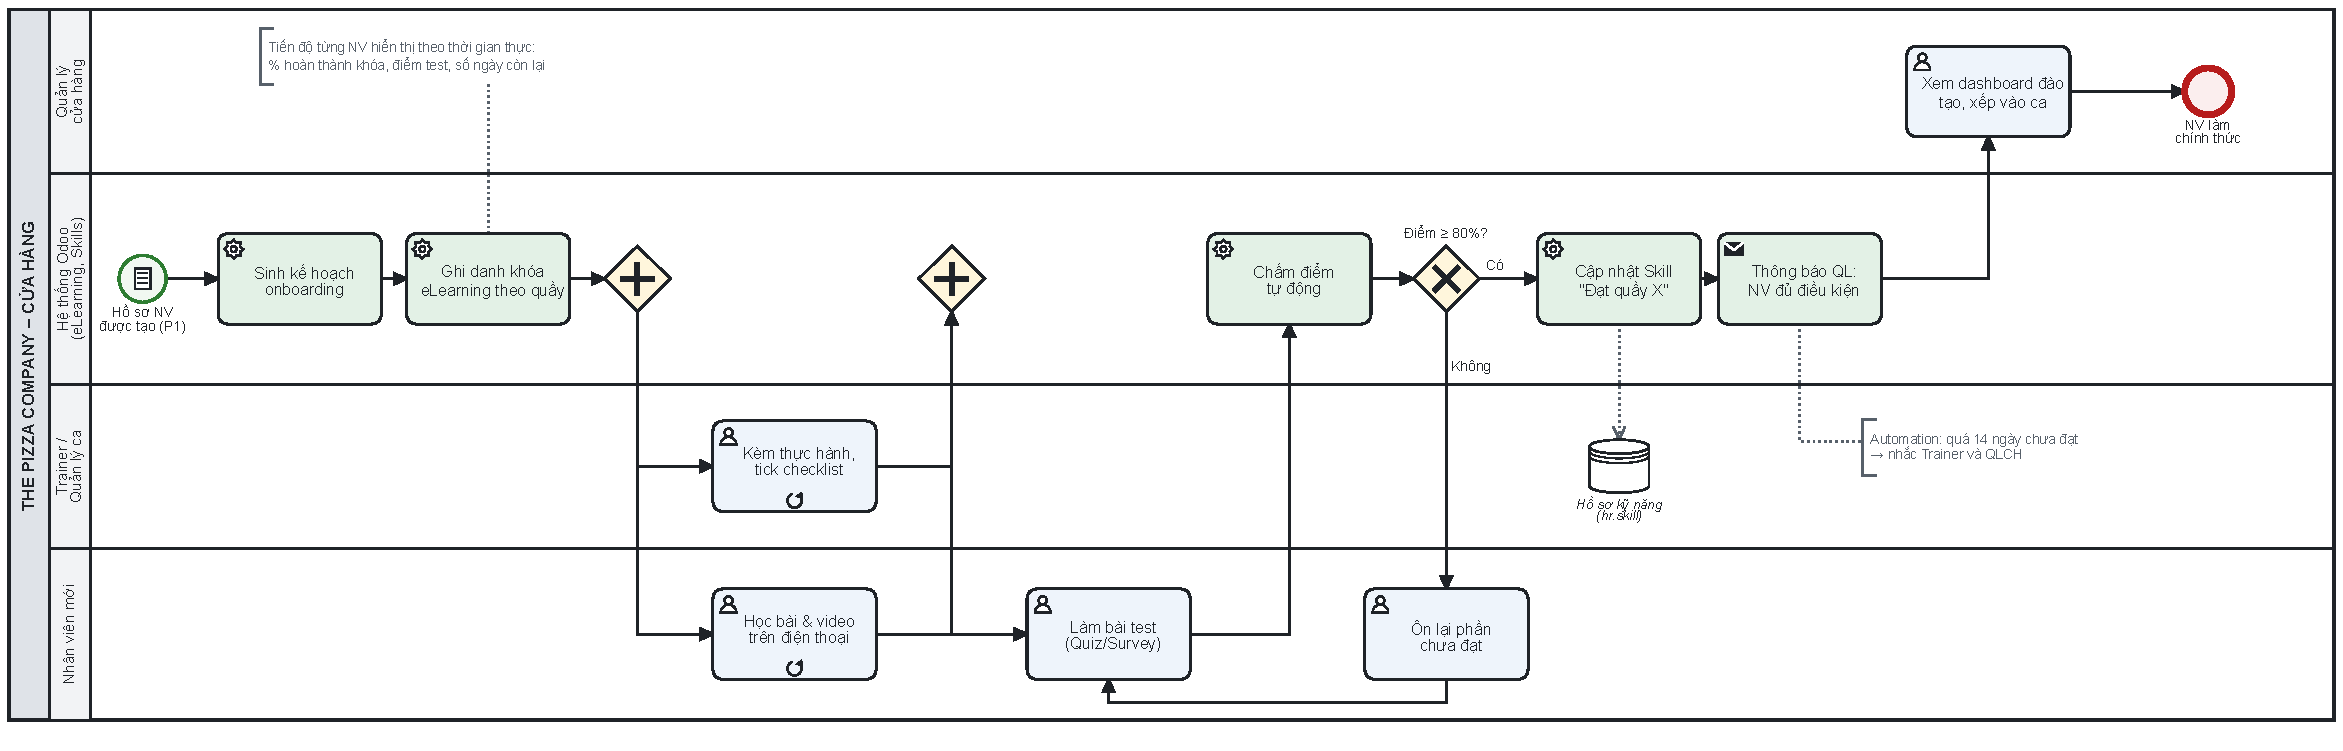
\includegraphics[width=\linewidth]{p2_tobe.pdf}
\caption{P2 – Quy trình onboarding và đào tạo đề xuất (TO-BE)}\label{fig:p2tobe}
\end{figure}
Khi hồ sơ nhân viên được tạo, hệ thống sinh kế hoạch onboarding và ghi danh khoá eLearning theo quầy (Hình~\ref{fig:p2tobe}). Nhân viên học bài, video trên điện thoại song song với việc trainer kèm thực hành và tick checklist. Bài test làm trên Quiz/Survey được chấm tự động; đạt $\geq$ 80\% thì hệ thống cập nhật kỹ năng ``Đạt quầy X'' và báo cho quản lý; chưa đạt thì giao ôn lại phần chưa đạt. Quá 14 ngày chưa đạt, hệ thống nhắc trainer và quản lý. \textbf{Thay đổi chính}: tiến độ từng người hiển thị theo thời gian thực; kỹ năng quầy trở thành dữ liệu dùng được cho xếp ca (P3).
\end{landscape}

\begin{landscape}
\subsection{P3 – Xếp ca theo dự báo doanh thu}
\begin{figure}[H]\centering
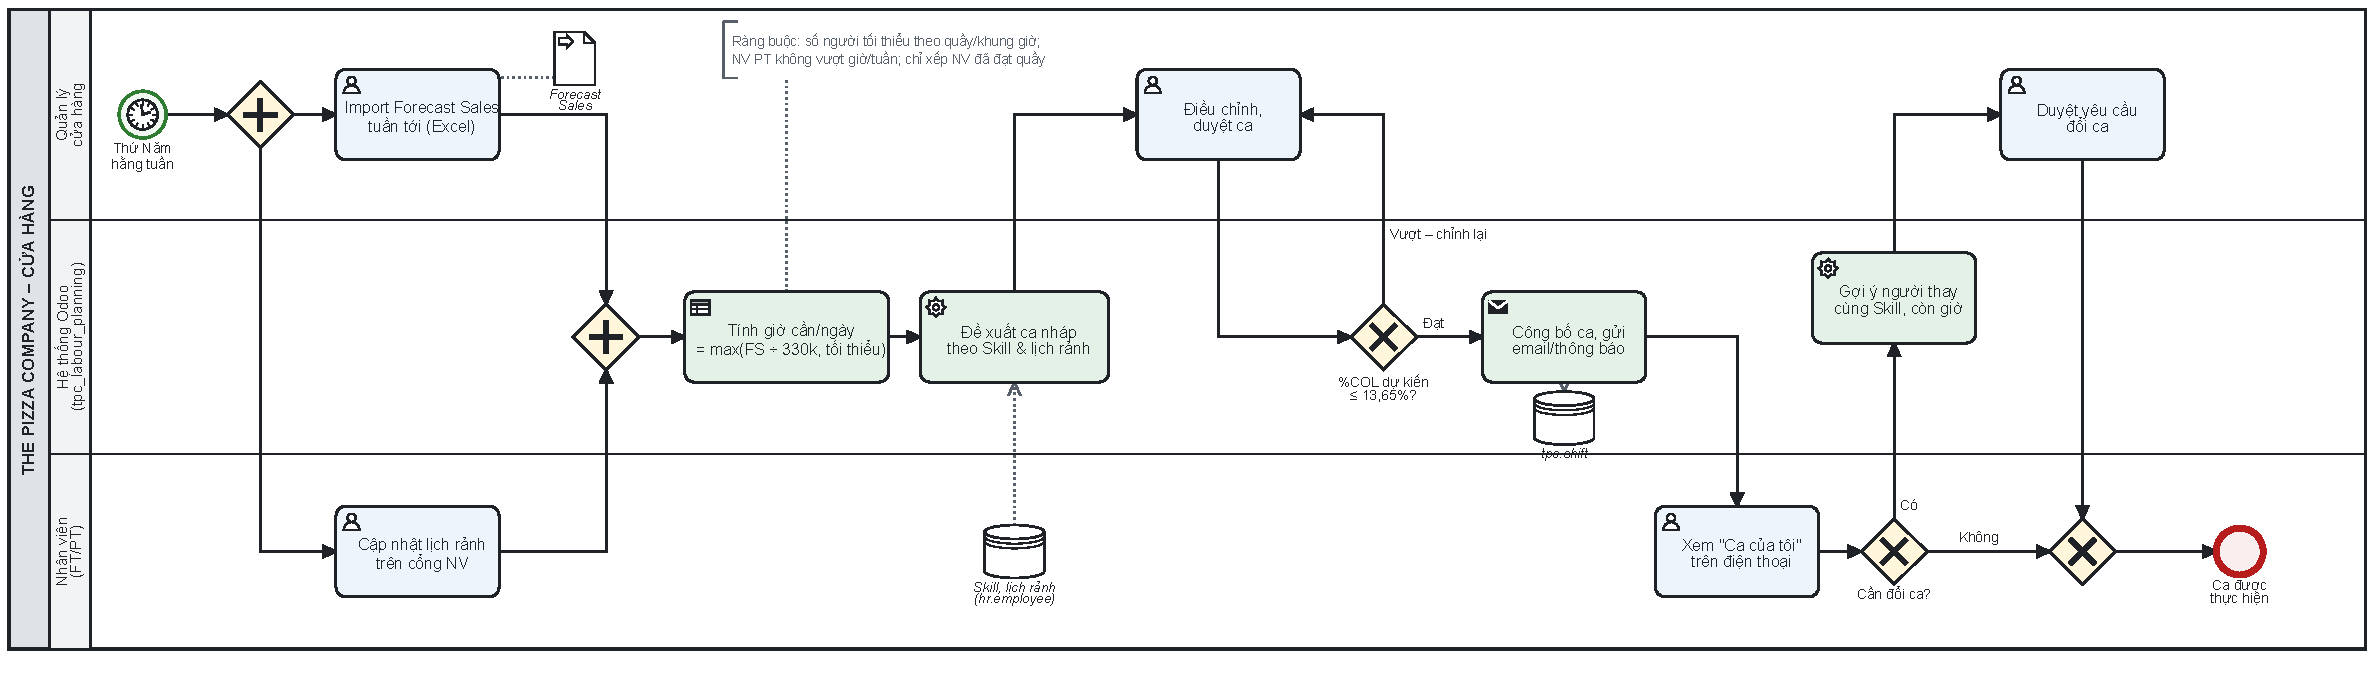
\includegraphics[width=\linewidth]{p3_tobe.pdf}
\caption{P3 – Quy trình xếp ca theo dự báo doanh thu (TO-BE, add-on \texttt{tpc\_labour\_planning})}\label{fig:p3tobe}
\end{figure}
Thứ Năm hằng tuần, quản lý import Forecast Sales tuần tới từ file Excel đúng mẫu công ty đang dùng; song song, nhân viên cập nhật lịch rảnh trên cổng nhân viên (Hình~\ref{fig:p3tobe}). Add-on tính giờ cần mỗi ngày theo quy tắc nghiệp vụ $\max(\text{Forecast Sales}/330.000,\ \text{giờ tối thiểu theo quầy})$, rồi đề xuất ca nháp, chỉ gán nhân viên đã đạt kỹ năng quầy, không vượt giờ tối đa của part-time. Quản lý điều chỉnh, duyệt; nếu \%COL dự kiến vượt 13,65\% thì phải chỉnh lại. Sau khi công bố, nhân viên xem ``Ca của tôi'' trên điện thoại; yêu cầu đổi ca được gửi trên hệ thống, hệ thống gợi ý người thay cùng kỹ năng, quản lý duyệt. \textbf{Thay đổi chính}: giờ công co giãn theo doanh thu, thiếu thừa được thấy \emph{trước} khi ca diễn ra.
\end{landscape}

\begin{landscape}
\subsection{P4 – Chấm công và theo dõi \%COL hằng ngày}
\begin{figure}[H]\centering
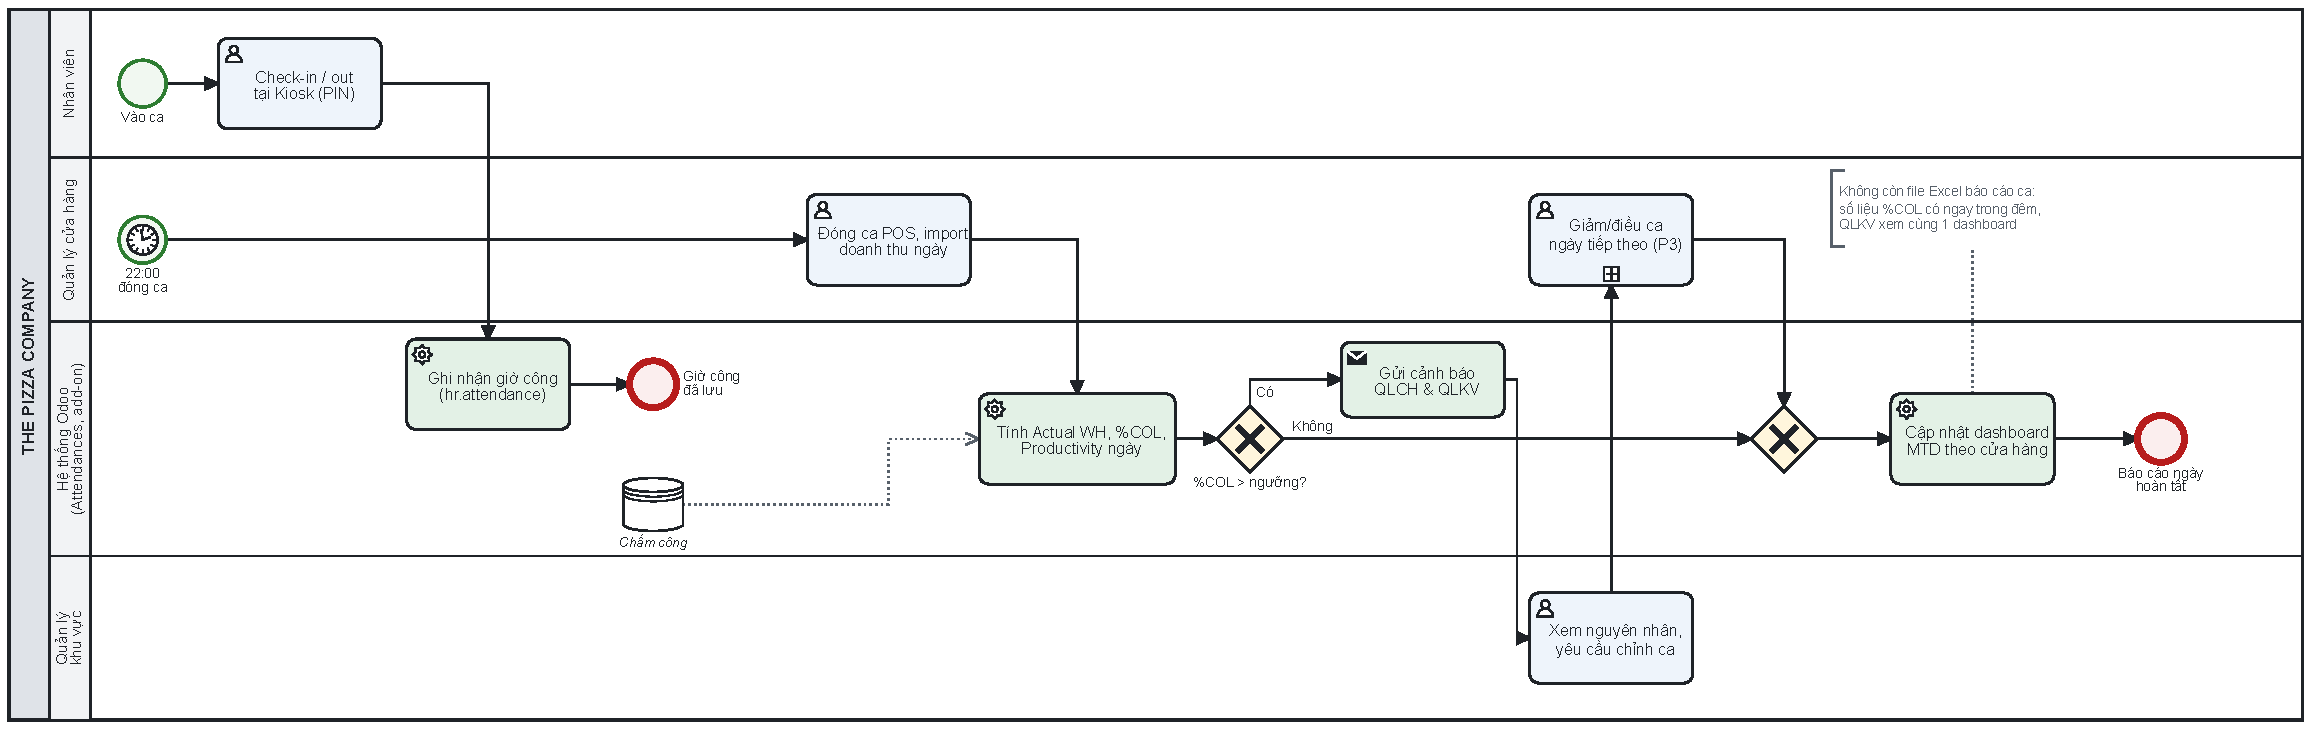
\includegraphics[width=\linewidth]{p4_tobe.pdf}
\caption{P4 – Quy trình chấm công và theo dõi \%COL hằng ngày (TO-BE)}\label{fig:p4tobe}
\end{figure}
Nhân viên check-in/out tại Kiosk (PIN hoặc badge), hệ thống ghi nhận giờ công (Hình~\ref{fig:p4tobe}). Khi đóng ca, quản lý import doanh thu ngày từ báo cáo POS; hệ thống tính Actual WH, \%COL, Productivity. Nếu \%COL vượt ngưỡng, hệ thống gửi cảnh báo cho quản lý cửa hàng và khu vực; quản lý khu vực xem nguyên nhân và yêu cầu điều chỉnh ca ngày tiếp theo (gọi lại P3). Dashboard MTD cập nhật thay cho việc nhập tay sheet \texttt{Store Perfomance}. \textbf{Thay đổi chính}: \%COL có ngay trong đêm thay vì cuối tháng.
\end{landscape}

\section{Bảng giá trị cải tiến (Value)}
\begin{longtable}{C{0.7cm}L{2.7cm}L{2.5cm}L{2.2cm}L{2.6cm}L{2.4cm}}
\caption{Giá trị cải tiến và cách đo}\label{tab:value}\\
\toprule \textbf{Mã} & \textbf{Giá trị} & \textbf{Chỉ số} & \textbf{Hiện tại} & \textbf{Mục tiêu} & \textbf{Cách chứng minh} \\\midrule\endfirsthead
\toprule \textbf{Mã} & \textbf{Giá trị} & \textbf{Chỉ số} & \textbf{Hiện tại} & \textbf{Mục tiêu} & \textbf{Cách chứng minh} \\\midrule\endhead
V1 & Rút ngắn thời gian tuyển (I1, I2) & Ngày từ nộp hồ sơ đến ca đầu & 2–4 ngày (sau PV) & 1–2 ngày & Demo luồng; QL xác nhận \\
V2 & Đào tạo đo lường được (I3) & \% NV đạt quầy đúng 14 ngày & Không đo được & Hiển thị theo thời gian thực & Dashboard eLearning, Skills \\
V3 & Giảm giờ công thừa (I4) & Giờ công/tháng, \%COL & T8: 5.882 giờ; 15,5\% & Trần tiết kiệm: 1.018 giờ ($\approx$ 41 tr.đ) nếu xếp đúng định mức; con số thực sau mô phỏng & Mô phỏng T8 bằng add-on (tuần 8) \\
V4 & Bổ sung người cho ngày đông & Giờ thiếu T7, CN & Thiếu $\sim$1.600 giờ/8 tháng & Giảm về $\approx$ 0 & Mô phỏng \\
V5 & Báo cáo \%COL tức thời (I6) & Thời gian có số \%COL & Cuối tháng & Trong ngày & Demo cron, dashboard \\
V6 & Đổi ca minh bạch (I5) & Số yêu cầu có lịch sử & 0\% & 100\% & Time Off log \\
V7 & Chủ động tuyển trước mùa nghỉ (I7) & Số NV tuyển trước tháng 2 & Bị động & Có kế hoạch & Báo cáo nghỉ việc theo tháng \\
\bottomrule
\end{longtable}

\begin{ghichu}[Về con số tiết kiệm]
Con số 1.018 giờ/tháng là \emph{giới hạn trên}, vì giả định ngày nào cũng xếp đúng định mức. Mức tiết kiệm thật phụ thuộc số người tối thiểu mỗi quầy và sẽ được tính bằng mô phỏng ở tuần 8. Báo cáo cuối kỳ chỉ dùng con số mô phỏng đã được doanh nghiệp xác nhận.
\end{ghichu}

\section{Yêu cầu hệ thống}
\subsection{Yêu cầu chức năng}
\begin{longtable}{C{1.1cm}L{9.4cm}C{1cm}C{1.6cm}}
\caption{Yêu cầu chức năng (M: Must, S: Should, C: Could)}\label{tab:fr}\\
\toprule \textbf{Mã} & \textbf{Mô tả} & \textbf{QT} & \textbf{Ưu tiên} \\\midrule\endfirsthead
\toprule \textbf{Mã} & \textbf{Mô tả} & \textbf{QT} & \textbf{Ưu tiên} \\\midrule\endhead
FR01 & Tạo vị trí tuyển dụng theo cửa hàng, số lượng cần tuyển, đăng lên trang Jobs & P1 & M \\
FR02 & Ứng viên nộp đơn online, kèm câu hỏi: ca muốn làm, khu vực, đã có TK Techcombank & P1 & M \\
FR03 & Pipeline 6 giai đoạn: Mới → Đã liên hệ → Hẹn PV → Đã PV → Đề nghị → Nhận việc & P1 & M \\
FR04 & Gắn nguồn ứng viên (Standee, Fanpage, Phòng TD, Giới thiệu, Website); báo cáo theo nguồn & P1 & M \\
FR05 & Gửi email tự động theo giai đoạn (xác nhận, mời PV, từ chối, chào mừng) & P1 & S \\
FR06 & Tạo hồ sơ nhân viên từ ứng viên, phòng NS duyệt và cấp mã & P1 & M \\
FR07 & Nhắc QLCH khi ứng viên ở giai đoạn Mới quá 48 giờ & P1 & C \\
FR08 & Khoá eLearning theo quầy, bài test chấm tự động, ngưỡng đạt 80\% & P2 & M \\
FR09 & Cập nhật kỹ năng ``Đạt quầy'' khi qua bài test; xem tiến độ đào tạo & P2 & M \\
FR10 & Nhắc trainer, QLCH khi quá 14 ngày chưa đạt & P2 & C \\
FR11 & Cấu hình định mức cửa hàng: Productivity, \%COL mục tiêu, lương TB/giờ, số người tối thiểu theo quầy & P3 & M \\
FR12 & Nhập tay hoặc import Forecast Sales theo ngày từ file Excel mẫu công ty & P3 & M \\
FR13 & Tính giờ công đề xuất mỗi ngày theo công thức và ràng buộc tối thiểu & P3 & M \\
FR14 & Tạo ca, gán NV; chỉ cho chọn NV đã đạt quầy; cảnh báo trùng ca, vượt giờ/tuần & P3 & M \\
FR15 & Đề xuất ca nháp tự động & P3 & S \\
FR16 & Công bố ca, NV xem ``Ca của tôi'' trên điện thoại & P3 & S \\
FR17 & NV gửi yêu cầu đổi ca; QLCH duyệt; lưu lịch sử & P3 & S \\
FR18 & Chấm công Kiosk bằng PIN/badge & P4 & M \\
FR19 & Báo cáo ngày: Actual WH, \%COL, Productivity, chênh lệch giờ; luỹ kế MTD & P4 & M \\
FR20 & Cron hằng đêm tính báo cáo, gửi cảnh báo khi \%COL vượt ngưỡng & P4 & S \\
FR21 & In bảng xếp ca tuần (PDF) & P3 & C \\
FR22 & Kết nối Power BI để xem dashboard khu vực & P4 & S \\
\bottomrule
\end{longtable}

\subsection{Yêu cầu phi chức năng}
\begin{itemize}
\item \textbf{Phân quyền}: nhân viên chỉ thấy ca, kỹ năng của mình; QLCH chỉ thấy dữ liệu cửa hàng mình; QLKV thấy các cửa hàng trong khu vực.
\item \textbf{Bảo mật dữ liệu cá nhân}: số điện thoại, tài khoản ngân hàng của NV, ứng viên chỉ phòng NS và QLCH xem được; dữ liệu demo dùng tên giả.
\item \textbf{Dễ dùng trên điện thoại}: cổng nhân viên, eLearning chạy tốt trên màn hình nhỏ.
\item \textbf{Hiệu năng}: tính giờ đề xuất cho 1 tuần, 1 cửa hàng dưới 5 giây; báo cáo ngày hoàn tất trước 23:30.
\item \textbf{Tương thích}: Odoo 18 Community; import file \texttt{.xlsx} đúng cấu trúc doanh nghiệp đang dùng.
\item \textbf{Sao lưu}: sao lưu CSDL hằng ngày; mã nguồn add-on quản lý trên GitHub.
\end{itemize}

\section{Các bên liên quan}
\begin{table}[H]\centering\small
\caption{Các bên liên quan và mối quan tâm}\label{tab:stake}
\begin{tabularx}{\linewidth}{L{3.3cm}YY}
\toprule \textbf{Bên liên quan} & \textbf{Vai trò trong hệ thống} & \textbf{Mối quan tâm chính} \\\midrule
Ban điều hành & Phê duyệt, tài trợ & Chi phí nhân công, đồng bộ chuỗi \\
Quản lý khu vực & Giám sát, cấu hình định mức & \%COL các cửa hàng, cảnh báo sớm \\
Quản lý cửa hàng & Người dùng chính & Tuyển nhanh, xếp ca nhanh, ít báo cáo tay \\
Quản lý ca / Trainer & Đào tạo, điều hành ca & Biết NV nào làm được quầy nào \\
Nhân viên part-time & Xem ca, học, chấm công & Lịch rõ ràng, đổi ca dễ \\
Ứng viên & Nộp đơn & Phản hồi nhanh, thủ tục gọn \\
Phòng Nhân sự – TD & Duyệt hồ sơ, cấp mã & Dữ liệu đầy đủ, không nhập lại \\
Bộ phận IT & Vận hành hệ thống & Bảo mật, sao lưu, tích hợp \\
\bottomrule
\end{tabularx}
\end{table}

\section{Sơ đồ use case và đặc tả}
\begin{figure}[H]\centering
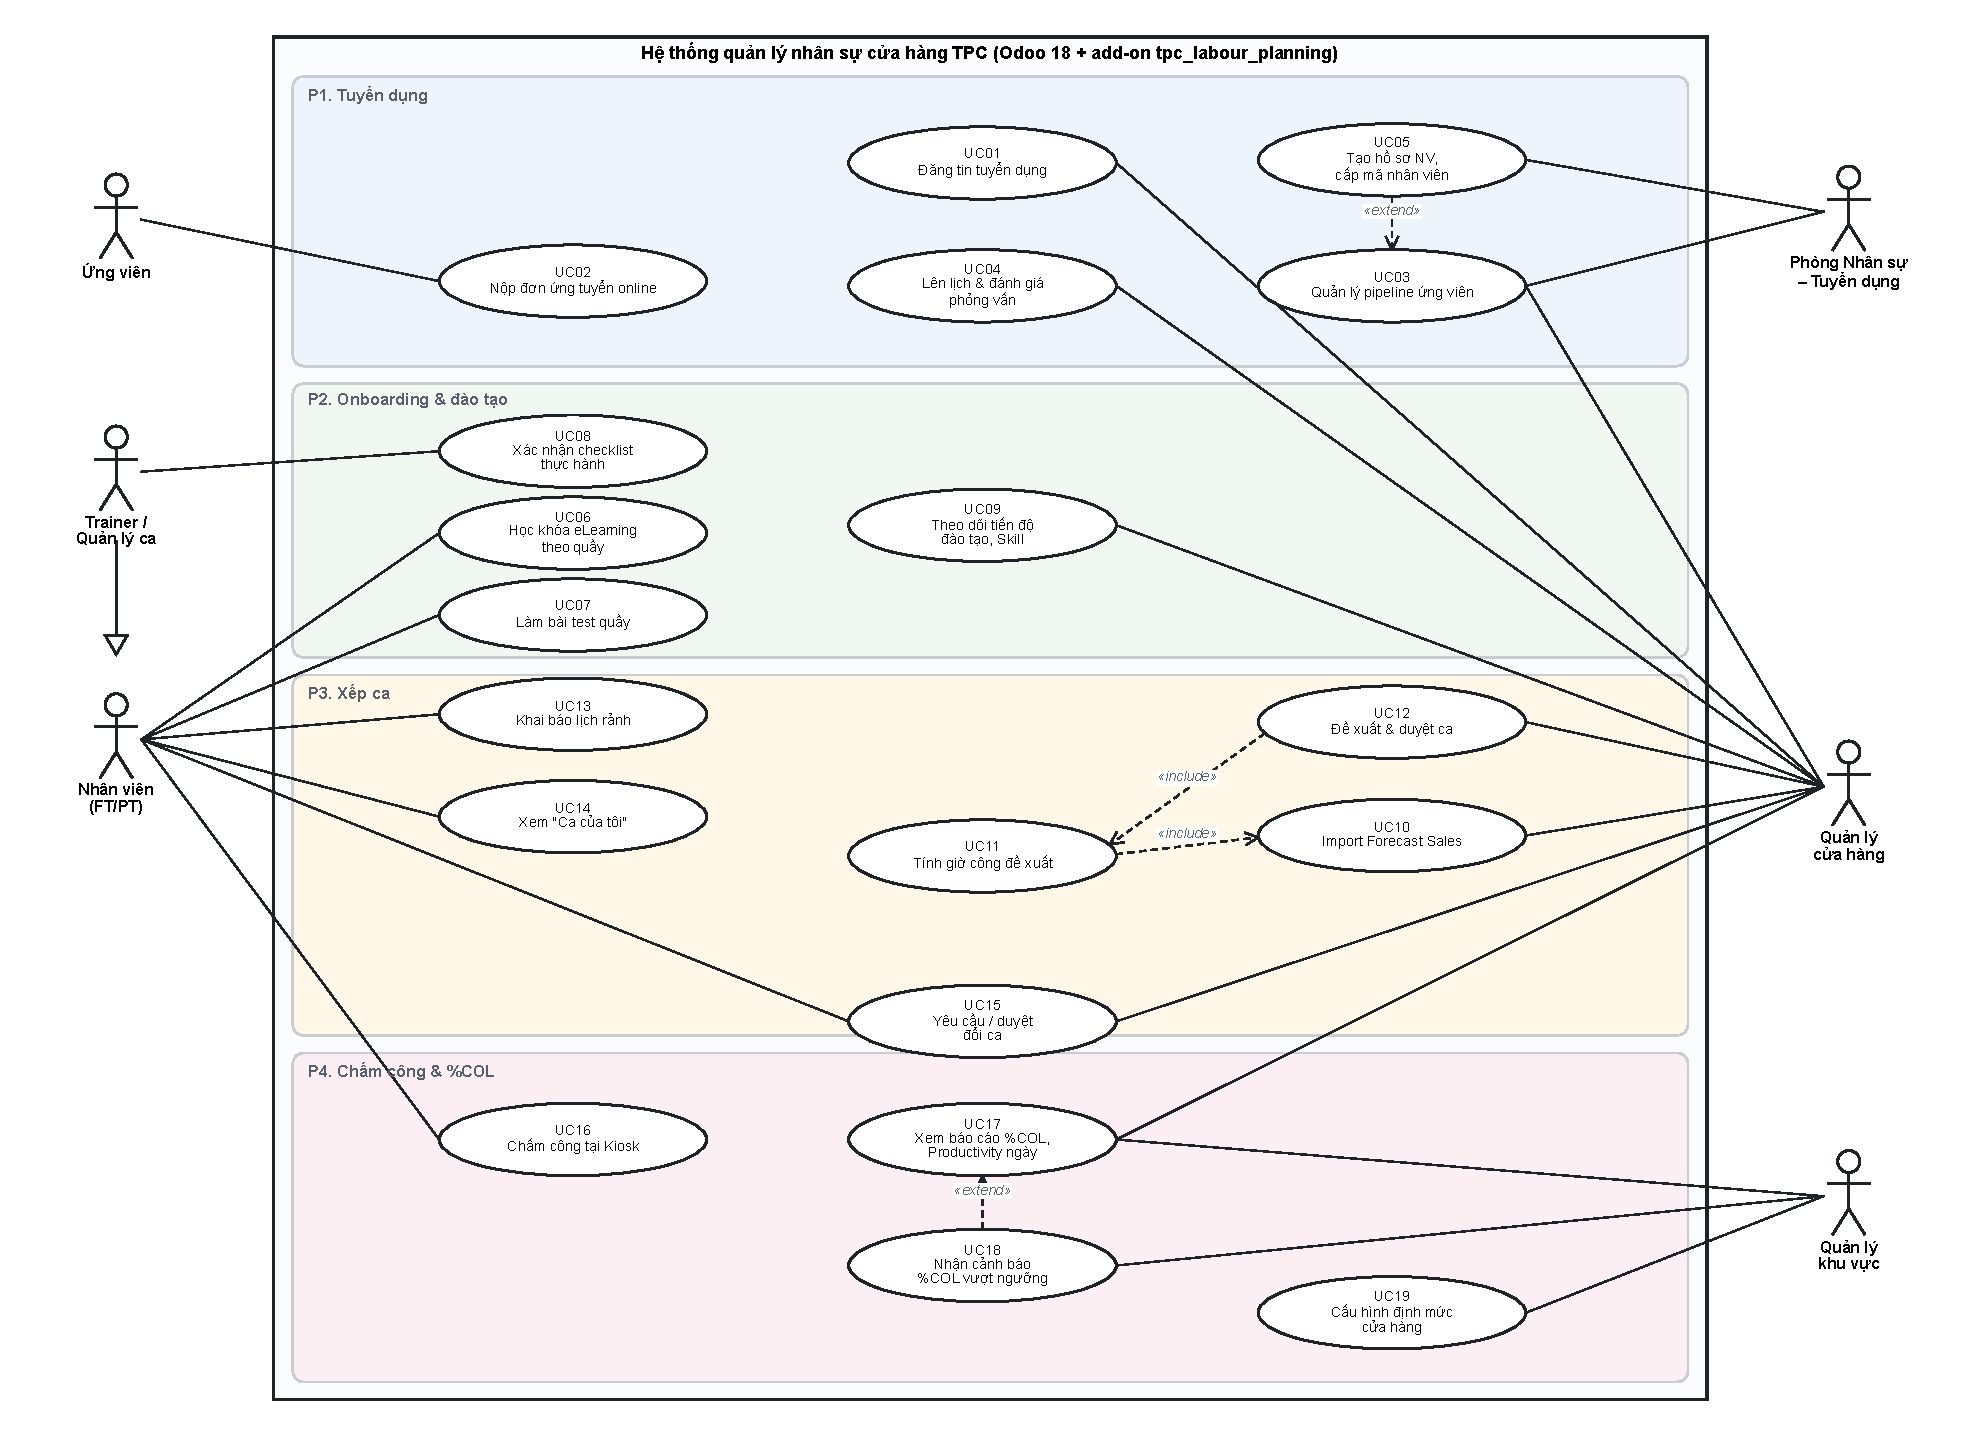
\includegraphics[width=\linewidth]{usecase.pdf}
\caption{Sơ đồ use case tổng quát}\label{fig:usecase}
\end{figure}

\begin{table}[H]\centering\small
\caption{Đặc tả UC11 – Tính giờ công đề xuất}\label{tab:uc11}
\begin{tabularx}{\linewidth}{L{3.2cm}Y}
\toprule
\textbf{Tác nhân} & Quản lý cửa hàng (gián tiếp qua UC12); cron hệ thống \\
\textbf{Mục tiêu} & Tính số giờ công cần cho từng ngày của tuần tới \\
\textbf{Tiền điều kiện} & Đã có Forecast Sales cho các ngày cần tính (UC10); cửa hàng đã cấu hình định mức (UC19) \\
\textbf{Luồng chính} & 1. QLCH chọn tuần và bấm ``Tính giờ''. 2. Với mỗi ngày, hệ thống lấy Forecast Sales $F$, Productivity mục tiêu $P$, giờ tối thiểu $H_{min}$ (tổng số người tối thiểu các quầy $\times$ số giờ mở cửa). 3. Giờ cần $H = \max(F/P, H_{min})$, làm tròn 0,5 giờ. 4. Tính \%COL dự kiến $= H\times\text{lương TB}/F$. 5. Hiển thị bảng theo ngày, tô đỏ ngày \%COL dự kiến vượt mục tiêu. \\
\textbf{Luồng phụ} & 2a. Thiếu Forecast của một ngày: dùng doanh thu cùng thứ của 4 tuần gần nhất và đánh dấu ``ước tính''. \\
\textbf{Hậu điều kiện} & Bản ghi \texttt{tpc.labour.daily} có \texttt{required\_hours} cho từng ngày \\
\textbf{Quy tắc} & BR1: $P$ mặc định 330.000 đ/giờ; BR2: \%COL mục tiêu 13,65\% \\
\bottomrule
\end{tabularx}
\end{table}

\begin{table}[H]\centering\small
\caption{Đặc tả UC12 – Đề xuất và duyệt ca}\label{tab:uc12}
\begin{tabularx}{\linewidth}{L{3.2cm}Y}
\toprule
\textbf{Tác nhân} & Quản lý cửa hàng \\
\textbf{Mục tiêu} & Có lịch ca tuần tới đủ giờ, đúng kỹ năng \\
\textbf{Tiền điều kiện} & UC11 đã chạy; NV đã khai báo lịch rảnh (UC13) \\
\textbf{Luồng chính} & 1. QLCH bấm ``Đề xuất ca''. 2. Hệ thống (include UC11) phân bổ giờ cần theo khung giờ và quầy. 3. Gán NV theo thứ tự: đã đạt quầy, có lịch rảnh, còn ít giờ nhất trong tuần. 4. Tạo ca trạng thái Nháp. 5. QLCH kéo thả, chỉnh sửa. 6. QLCH bấm ``Công bố''; ca chuyển sang Đã công bố, NV nhận thông báo. \\
\textbf{Luồng phụ} & 3a. Không đủ NV đạt quầy: để trống ca và cảnh báo ``thiếu người quầy X''. 6a. \%COL dự kiến vượt mục tiêu: hiện cảnh báo, QLCH phải ghi lý do nếu vẫn công bố. \\
\textbf{Hậu điều kiện} & Các bản ghi \texttt{tpc.shift} đã công bố cho tuần tới \\
\bottomrule
\end{tabularx}
\end{table}

\begin{table}[H]\centering\small
\caption{Đặc tả UC02 – Nộp đơn ứng tuyển online}\label{tab:uc02}
\begin{tabularx}{\linewidth}{L{3.2cm}Y}
\toprule
\textbf{Tác nhân} & Ứng viên \\
\textbf{Luồng chính} & 1. Ứng viên mở trang Jobs, chọn vị trí. 2. Điền họ tên, SĐT, email, ca muốn làm, khu vực, đã có TK Techcombank chưa. 3. Gửi đơn. 4. Hệ thống tạo hồ sơ ở giai đoạn Mới, nguồn Website, gửi email xác nhận. \\
\textbf{Luồng phụ} & 2a. Thiếu trường bắt buộc: báo lỗi tại trường. 4a. SĐT trùng ứng viên cũ: gộp vào hồ sơ cũ và báo QLCH. \\
\textbf{Hậu điều kiện} & Ứng viên xuất hiện trong pipeline của cửa hàng \\
\bottomrule
\end{tabularx}
\end{table}

\begin{table}[H]\centering\small
\caption{Đặc tả UC17 – Xem báo cáo \%COL ngày}\label{tab:uc17}
\begin{tabularx}{\linewidth}{L{3.2cm}Y}
\toprule
\textbf{Tác nhân} & Quản lý cửa hàng, Quản lý khu vực \\
\textbf{Tiền điều kiện} & Doanh thu ngày đã được import; có dữ liệu chấm công \\
\textbf{Luồng chính} & 1. Người dùng mở ``Báo cáo nhân công''. 2. Hệ thống hiển thị theo ngày: doanh thu, giờ đề xuất, giờ thực tế, chênh lệch, \%COL, Productivity và luỹ kế MTD. 3. Người dùng lọc theo cửa hàng, tuần, thứ; chuyển dạng pivot/biểu đồ. \\
\textbf{Mở rộng} & UC18: khi \%COL ngày vượt ngưỡng, cron gửi email cảnh báo kèm liên kết đến báo cáo. \\
\textbf{Phân quyền} & QLCH chỉ thấy cửa hàng mình; QLKV thấy các cửa hàng trong khu vực \\
\bottomrule
\end{tabularx}
\end{table}

\section{Thiết kế logic}
Sơ đồ lớp (Hình~\ref{fig:class}) gồm các lớp có sẵn trong Odoo được mở rộng thêm field (nền xanh dương) và các lớp mới của add-on (nền xanh lá). Lớp trung tâm là \textbf{LabourDaily}, tổng hợp từ SalesForecast (doanh thu), Shift (giờ đề xuất) và Attendance (giờ thực tế) để tính \%COL, Productivity mỗi ngày. Lớp \textbf{StationSkill} nối P2 với P3: kết quả đào tạo trở thành điều kiện để được xếp vào ca của quầy.

\begin{figure}[H]\centering
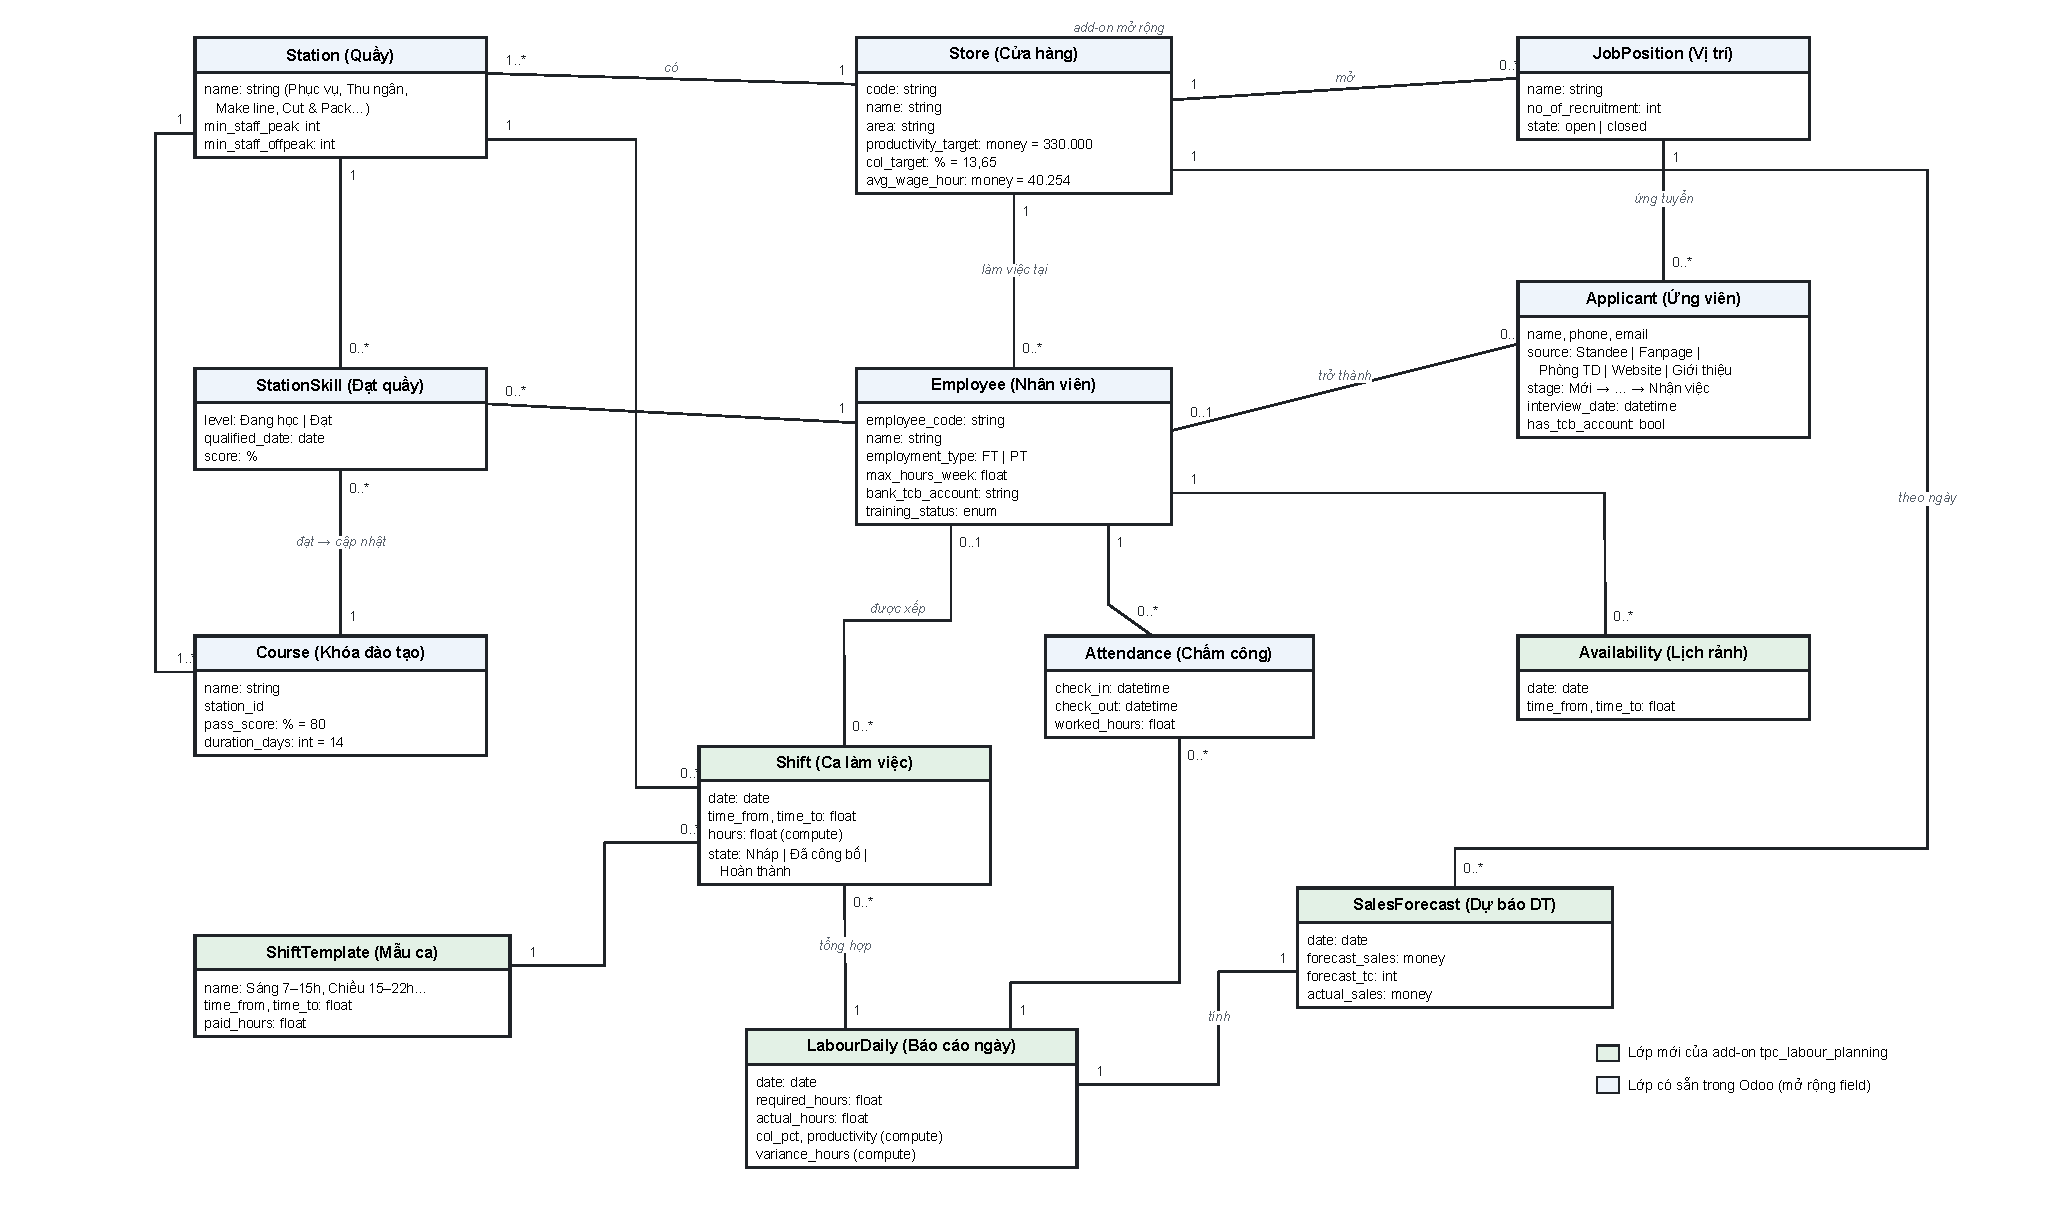
\includegraphics[width=\linewidth]{class_diagram.pdf}
\caption{Sơ đồ lớp mức logic}\label{fig:class}
\end{figure}

\section{Thiết kế vật lý}
\subsection{Kiến trúc triển khai}
\begin{figure}[H]\centering
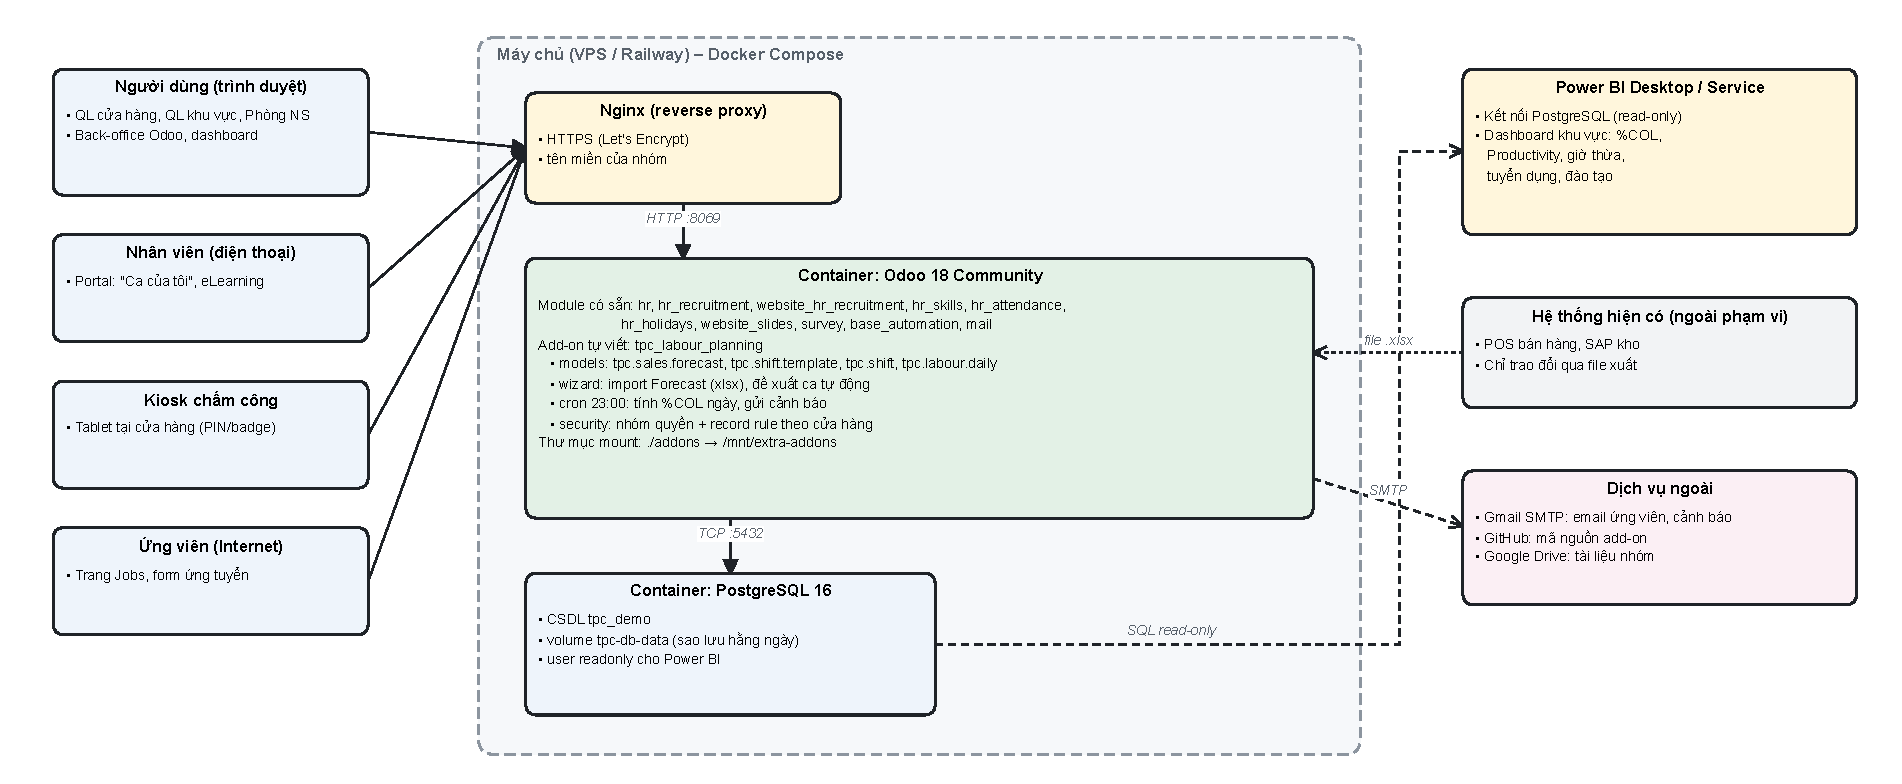
\includegraphics[width=\linewidth]{architecture.pdf}
\caption{Kiến trúc triển khai (physical)}\label{fig:arch}
\end{figure}

\subsection{Ánh xạ sang model Odoo}
\begin{longtable}{L{3.2cm}L{4.4cm}L{6.8cm}}
\caption{Ánh xạ lớp logic sang model Odoo}\label{tab:map}\\
\toprule \textbf{Lớp logic} & \textbf{Model Odoo} & \textbf{Ghi chú / field tuỳ biến} \\\midrule\endfirsthead
\toprule \textbf{Lớp logic} & \textbf{Model Odoo} & \textbf{Ghi chú / field tuỳ biến} \\\midrule\endhead
Store & \texttt{res.company} (mỗi cửa hàng 1 công ty con) & \texttt{x\_productivity\_target}, \texttt{x\_col\_target}, \texttt{x\_avg\_wage\_hour}; record rule đa công ty \\
Station & \texttt{hr.skill} (loại ``Quầy làm việc'') & Thêm \texttt{x\_min\_staff\_peak}, \texttt{x\_min\_staff\_offpeak} \\
StationSkill & \texttt{hr.employee.skill} & Cấp độ: Đang học (30\%), Đạt (100\%) \\
Employee & \texttt{hr.employee} & \texttt{x\_employment\_type} (FT/PT), \texttt{x\_max\_hours\_week}, \texttt{x\_bank\_tcb\_account} \\
JobPosition & \texttt{hr.job} & Đăng website (\texttt{is\_published}) \\
Applicant & \texttt{hr.applicant} (+ \texttt{hr.candidate}) & Nguồn: \texttt{utm.source}; câu hỏi form: \texttt{x\_preferred\_shift}, \texttt{x\_has\_tcb} \\
Course & \texttt{slide.channel} + \texttt{survey.survey} & Mỗi quầy 1 khoá; quiz ngưỡng 80\% \\
Attendance & \texttt{hr.attendance} & Kiosk mode, PIN \\
Availability & \texttt{tpc.availability} (mới) & NV khai trên portal \\
SalesForecast & \texttt{tpc.sales.forecast} (mới) & Unique (cửa hàng, ngày); wizard import xlsx \\
ShiftTemplate & \texttt{tpc.shift.template} (mới) & Ca sáng, chiều, gãy, cao điểm \\
Shift & \texttt{tpc.shift} (mới) & Calendar view; ràng buộc kỹ năng, trùng ca \\
LabourDaily & \texttt{tpc.labour.daily} (mới) & Compute \%COL, Productivity; pivot/graph; cron \\
Đổi ca & \texttt{hr.leave} (loại ``Xin đổi ca'') & Duyệt 1 cấp: QLCH \\
\bottomrule
\end{longtable}

\subsection{Ma trận phân quyền}
\begin{table}[H]\centering\small
\caption{Ma trận phân quyền (C: tạo, R: đọc, U: sửa, D: xoá; ``own'': chỉ bản ghi của mình; ``store'': chỉ cửa hàng mình)}\label{tab:acl}
\begin{tabular}{lccccc}
\toprule \textbf{Đối tượng} & \textbf{NV} & \textbf{QL ca/Trainer} & \textbf{QLCH} & \textbf{Phòng NS} & \textbf{QLKV} \\\midrule
Ứng viên & – & R (store) & CRUD (store) & CRUD & R \\
Hồ sơ nhân viên & R (own) & R (store) & RU (store) & CRUD & R \\
Kỹ năng quầy & R (own) & CRU (store) & CRUD (store) & R & R \\
Forecast Sales & – & R (store) & CRUD (store) & – & CRUD \\
Ca làm việc & R (own) & RU (store) & CRUD (store) & R & R \\
Lịch rảnh & CRUD (own) & R (store) & R (store) & – & – \\
Chấm công & C (own, kiosk) & RU (store) & RU (store) & R & R \\
Báo cáo ngày & – & R (store) & R (store) & – & R \\
Định mức cửa hàng & – & – & R & – & CRUD \\
\bottomrule
\end{tabular}
\end{table}

\subsection{Danh sách module}
\begin{table}[H]\centering\small
\caption{Module Odoo sử dụng}\label{tab:modules}
\begin{tabularx}{\linewidth}{L{4.6cm}YC{2.3cm}}
\toprule \textbf{Module (kỹ thuật)} & \textbf{Mục đích} & \textbf{Phiên bản} \\\midrule
\texttt{hr} & Hồ sơ nhân viên, phòng ban, vị trí & Community \\
\texttt{hr\_recruitment} & Pipeline ứng viên, email theo giai đoạn & Community \\
\texttt{website\_hr\_recruitment} & Trang Jobs, form ứng tuyển & Community \\
\texttt{hr\_skills} & Kỹ năng quầy & Community \\
\texttt{website\_slides}, \texttt{survey} & eLearning, bài test & Community \\
\texttt{hr\_attendance} & Chấm công, Kiosk & Community \\
\texttt{hr\_holidays} & Nghỉ phép, xin đổi ca & Community \\
\texttt{base\_automation} & Quy tắc tự động (nhắc 48 giờ, 14 ngày) & Community \\
\texttt{tpc\_labour\_planning} & Dự báo, xếp ca, báo cáo \%COL & Tự viết \\
Planning, Approvals, Studio & Không dùng (thay bằng add-on) & Enterprise \\
\bottomrule
\end{tabularx}
\end{table}

% =====================================================================
\chapter{Triển khai Odoo (giai đoạn tuần 1–4)}
% =====================================================================

\section{Cài đặt Odoo 18 Community bằng Docker}
Môi trường: macOS, Docker Desktop. Thư mục \texttt{odoo/} của dự án gồm \texttt{docker-compose.yml}, \texttt{config/odoo.conf} và \texttt{addons/} (nơi đặt add-on tự viết). Chạy \texttt{docker compose up -d}, Odoo phục vụ tại \url{http://localhost:8069}.

\lstinputlisting[language={},caption={docker-compose.yml},label=lst:compose]{../odoo/docker-compose.yml}

\lstinputlisting[language={},caption={config/odoo.conf},label=lst:conf]{../odoo/config/odoo.conf}

\begin{canxacnhan}[Bảo mật]
Mật khẩu trong file cấu hình chỉ dùng cho máy cá nhân. Khi triển khai lên máy chủ (tuần 6), đổi \texttt{admin\_passwd}, mật khẩu PostgreSQL, tài khoản admin và đặt sau Nginx có HTTPS.
\end{canxacnhan}

\section{Tạo cơ sở dữ liệu và cài module}
Cơ sở dữ liệu \texttt{tpc\_demo} được tạo bằng script \texttt{odoo/scripts/setup\_db.py} (gọi API XML-RPC của Odoo): ngôn ngữ Tiếng Việt, quốc gia Việt Nam, không nạp dữ liệu mẫu. Script cài lần lượt 10 module (Bảng~\ref{tab:modules}); thời gian cài mỗi module 1–6 giây. Dùng script thay vì bấm tay giúp cả nhóm dựng lại môi trường giống hệt nhau trên máy mỗi người.

\section{Cấu hình Employees, Recruitment và Skills}
Script \texttt{odoo/scripts/configure\_hr.py} cấu hình theo thiết kế ở Chương 4:
\begin{itemize}
\item Công ty ``TPC – Cửa hàng demo LVS'', tiền tệ VND, múi giờ Asia/Ho\_Chi\_Minh.
\item 5 phòng ban: Phục vụ, Thu ngân, Bếp, Giao hàng, Quản lý cửa hàng.
\item 5 vị trí: Phục vụ part-time, Thu ngân part-time, Bếp part-time (Make line / Cut \& Pack), Giao hàng, Shift Manager; 4 vị trí đầu đăng trên trang Jobs.
\item 6 giai đoạn tuyển dụng đúng quy trình TO-BE (Mới → Đã liên hệ → Hẹn phỏng vấn → Đã phỏng vấn → Đề nghị nhận việc → Nhận việc).
\item 5 nguồn ứng viên: Standee, Fanpage, Phòng Tuyển dụng gửi, Người quen giới thiệu, Website Jobs.
\item Loại kỹ năng ``Quầy làm việc'' với 6 kỹ năng (Phục vụ, Thu ngân, Bếp – Make line, Bếp – Cut \& Pack, Giao hàng, ATVSTP) và 2 cấp độ (Đang học, Đạt).
\item Dữ liệu demo: 24 nhân viên và 19 ứng viên, \textbf{tên giả sinh ngẫu nhiên}, email dạng \texttt{@example.com}.
\end{itemize}

\begin{figure}[H]\centering
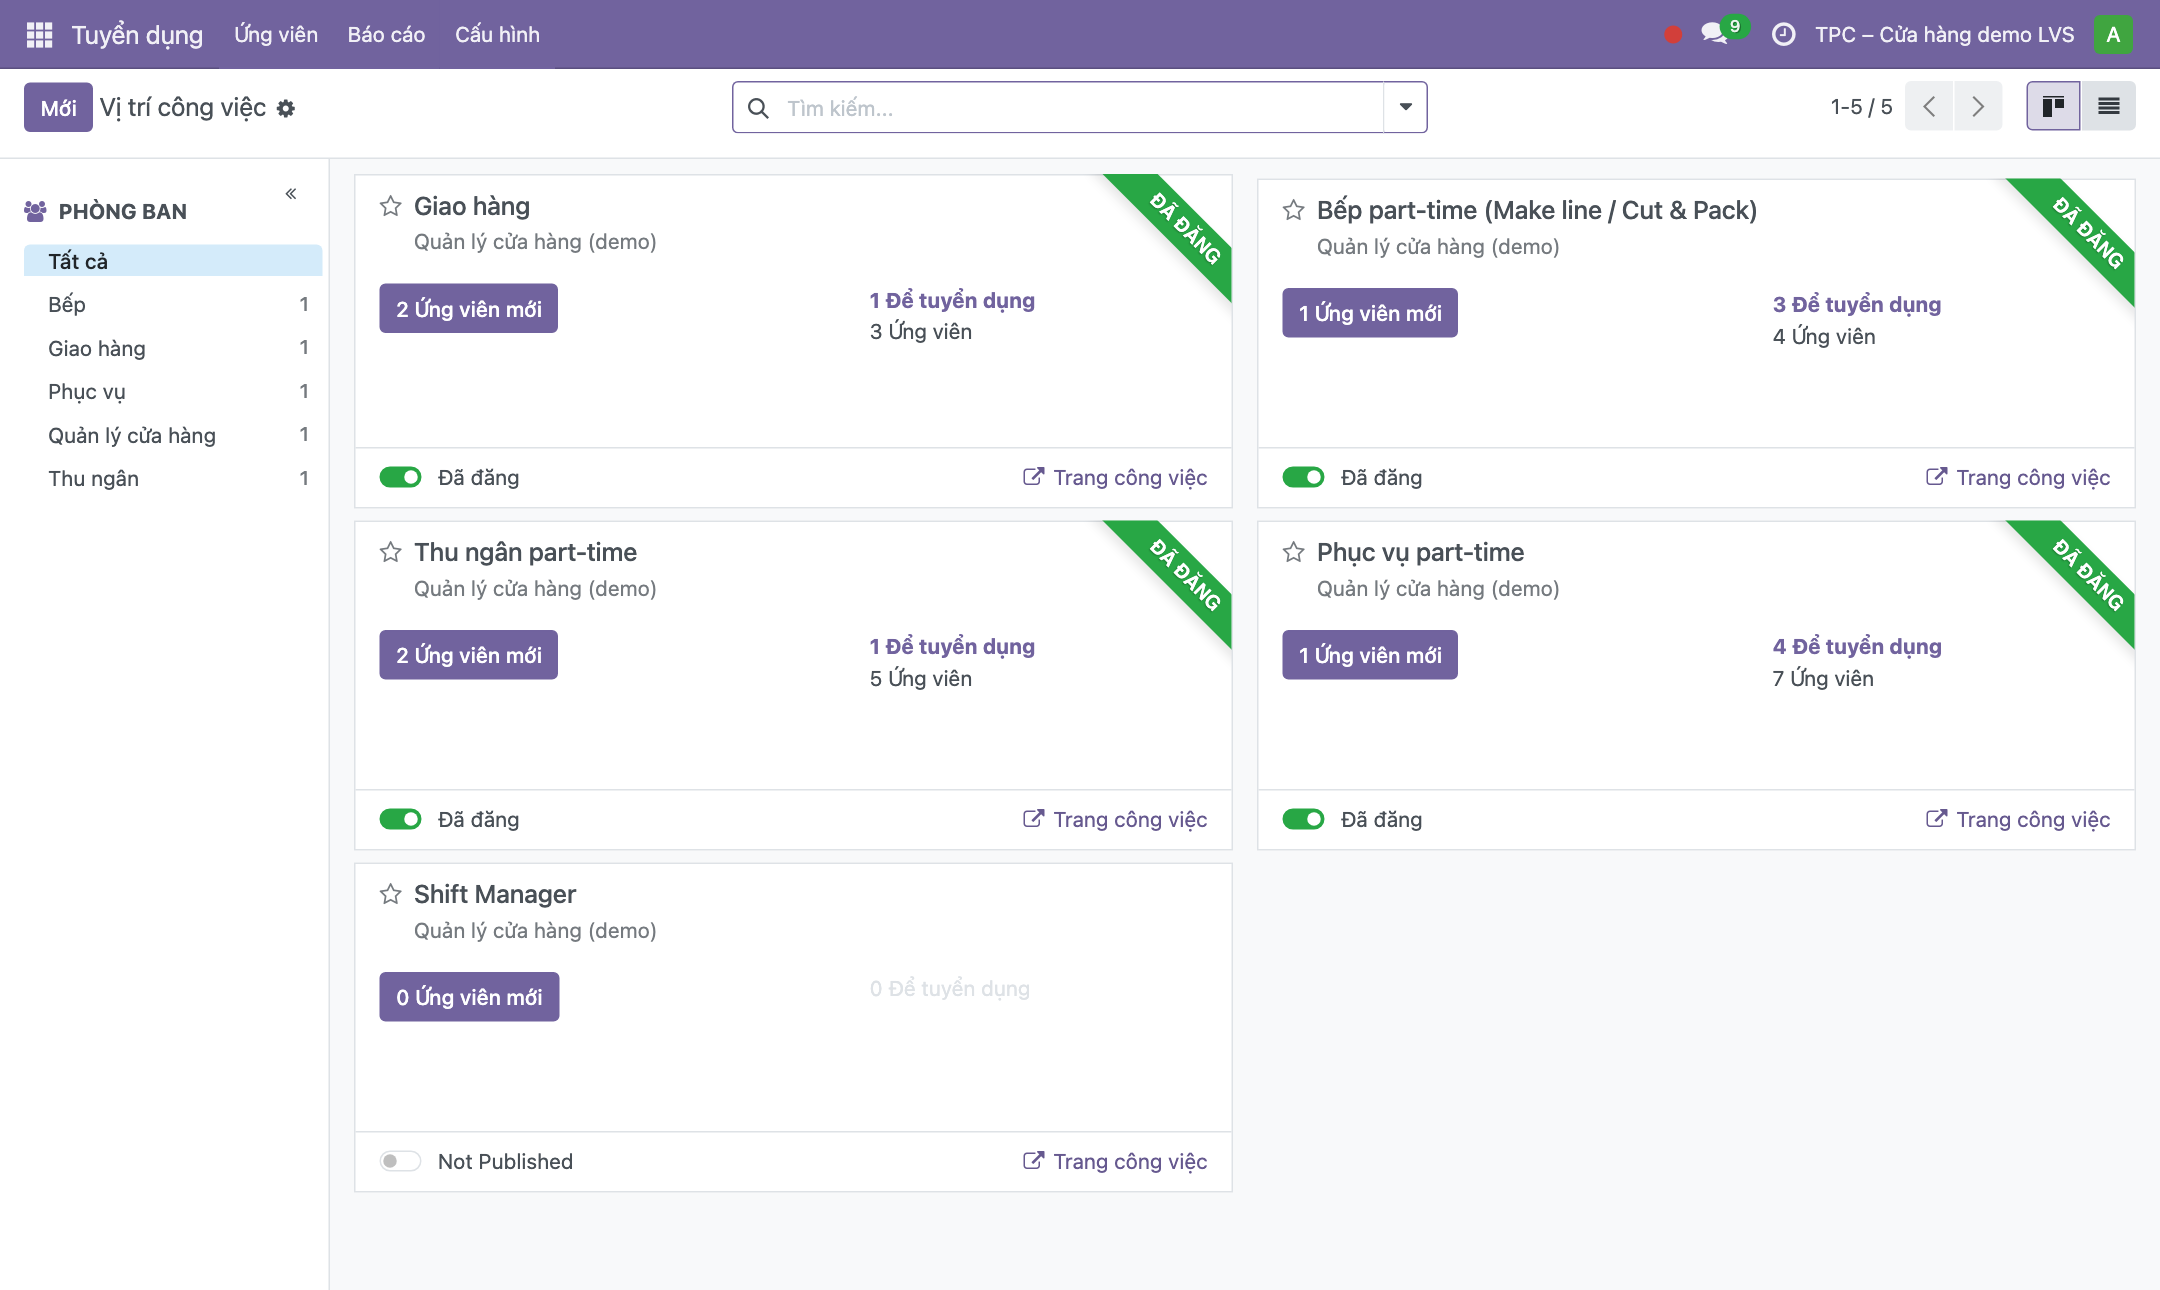
\includegraphics[width=\linewidth]{odoo/recruit_jobs.png}
\caption{Odoo Recruitment – các vị trí đang tuyển của cửa hàng demo}\label{fig:od_jobs}
\end{figure}
\begin{figure}[H]\centering
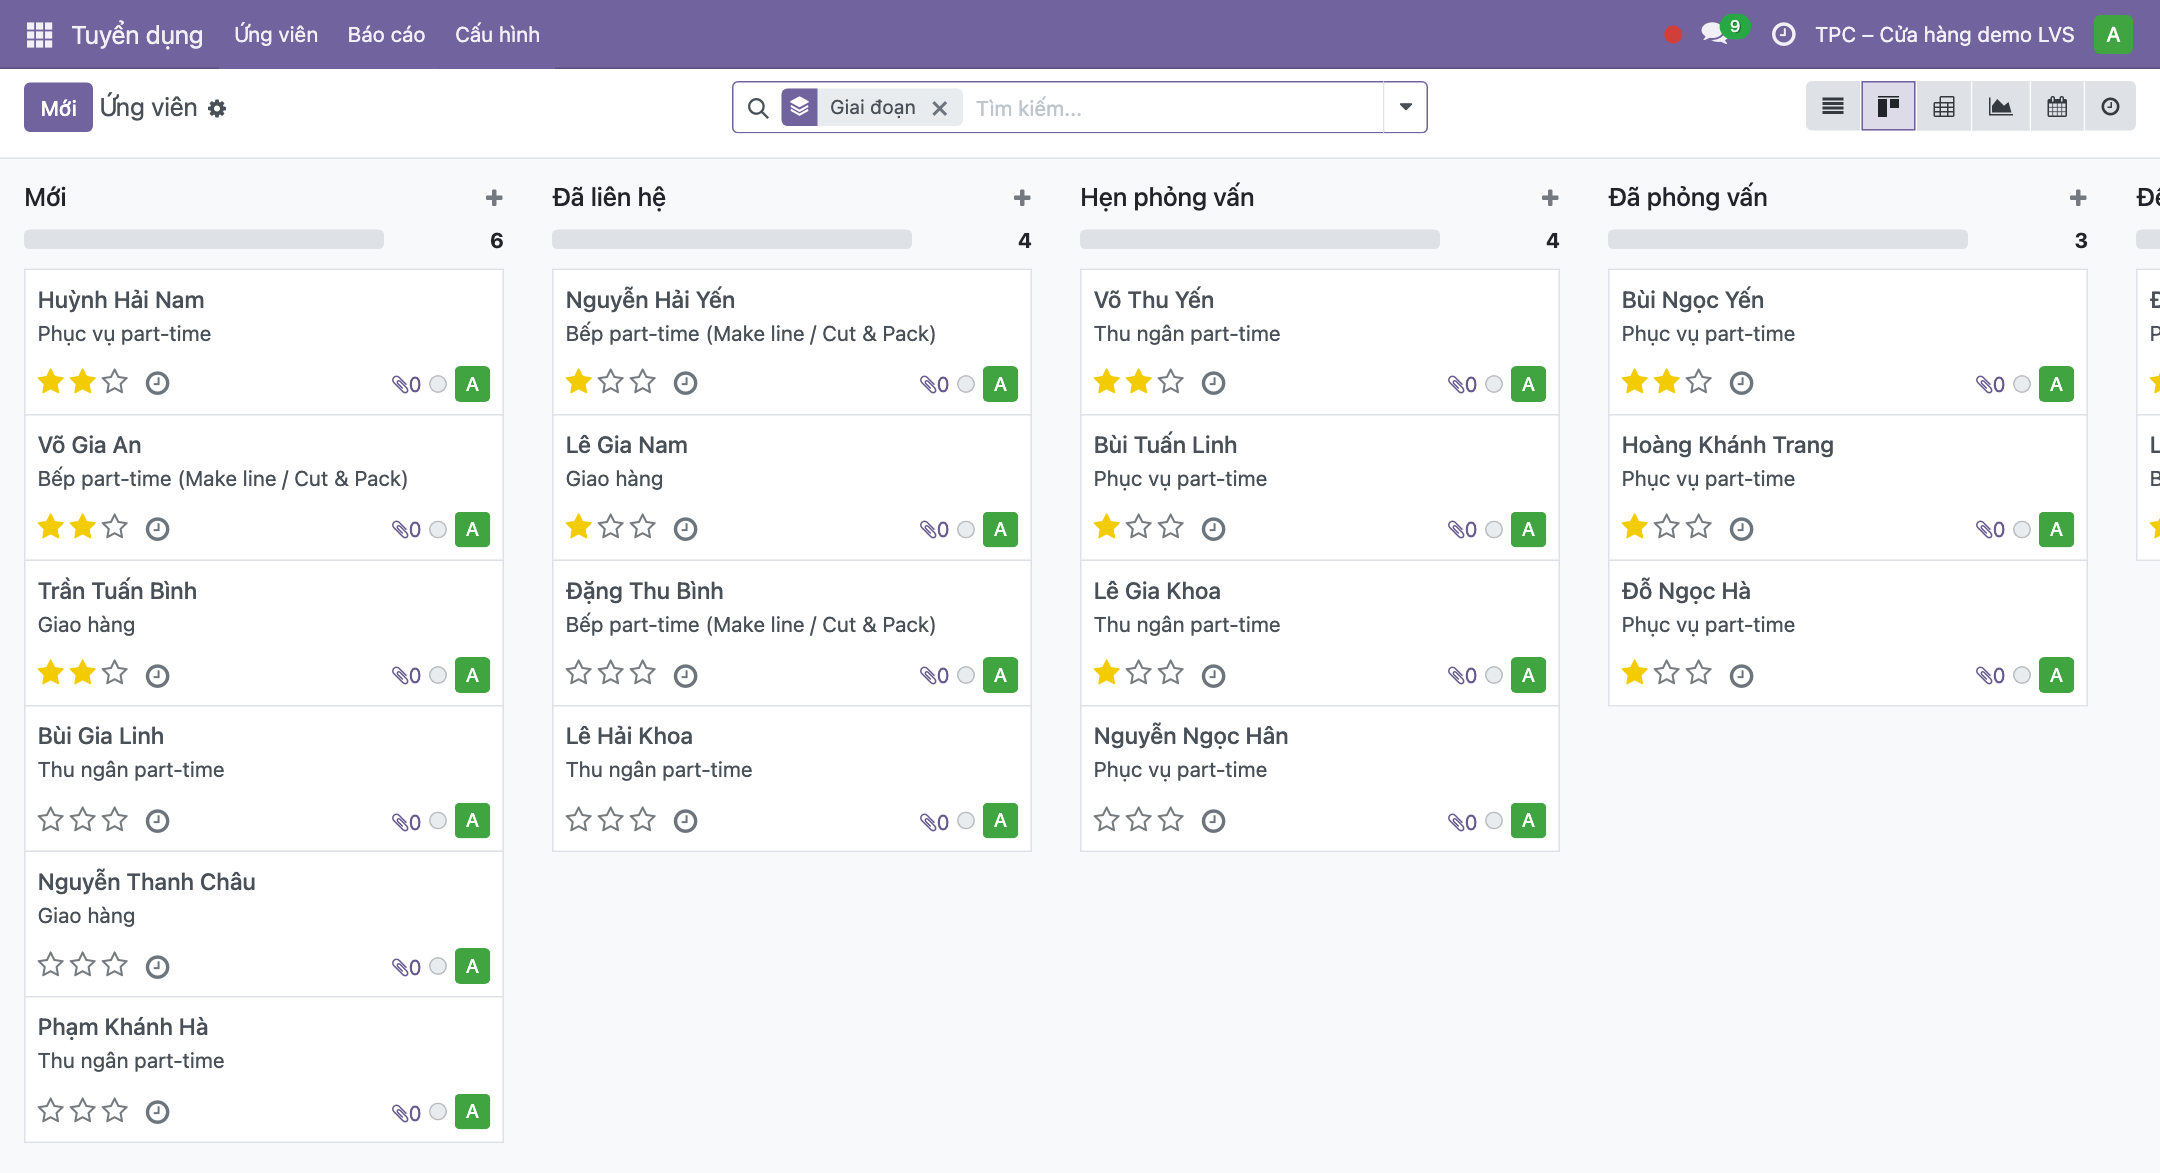
\includegraphics[width=\linewidth]{odoo/pipeline_kanban2.png}
\caption{Pipeline ứng viên theo 6 giai đoạn TO-BE (dữ liệu giả)}\label{fig:od_pipe}
\end{figure}
\begin{figure}[H]\centering
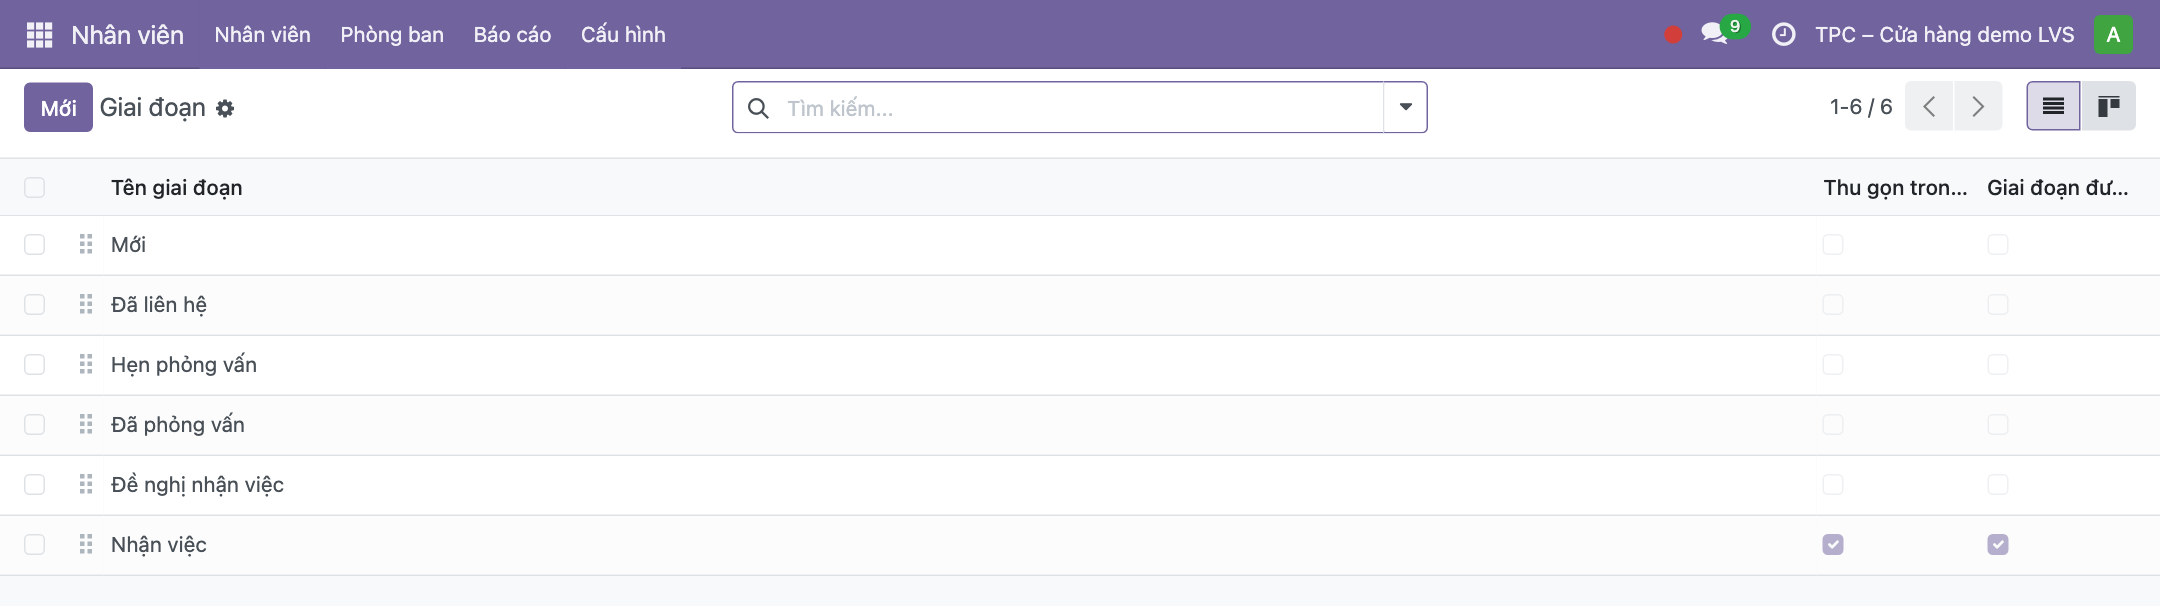
\includegraphics[width=\linewidth]{odoo/stages.png}
\caption{Cấu hình giai đoạn tuyển dụng}\label{fig:od_stages}
\end{figure}
\begin{figure}[H]\centering
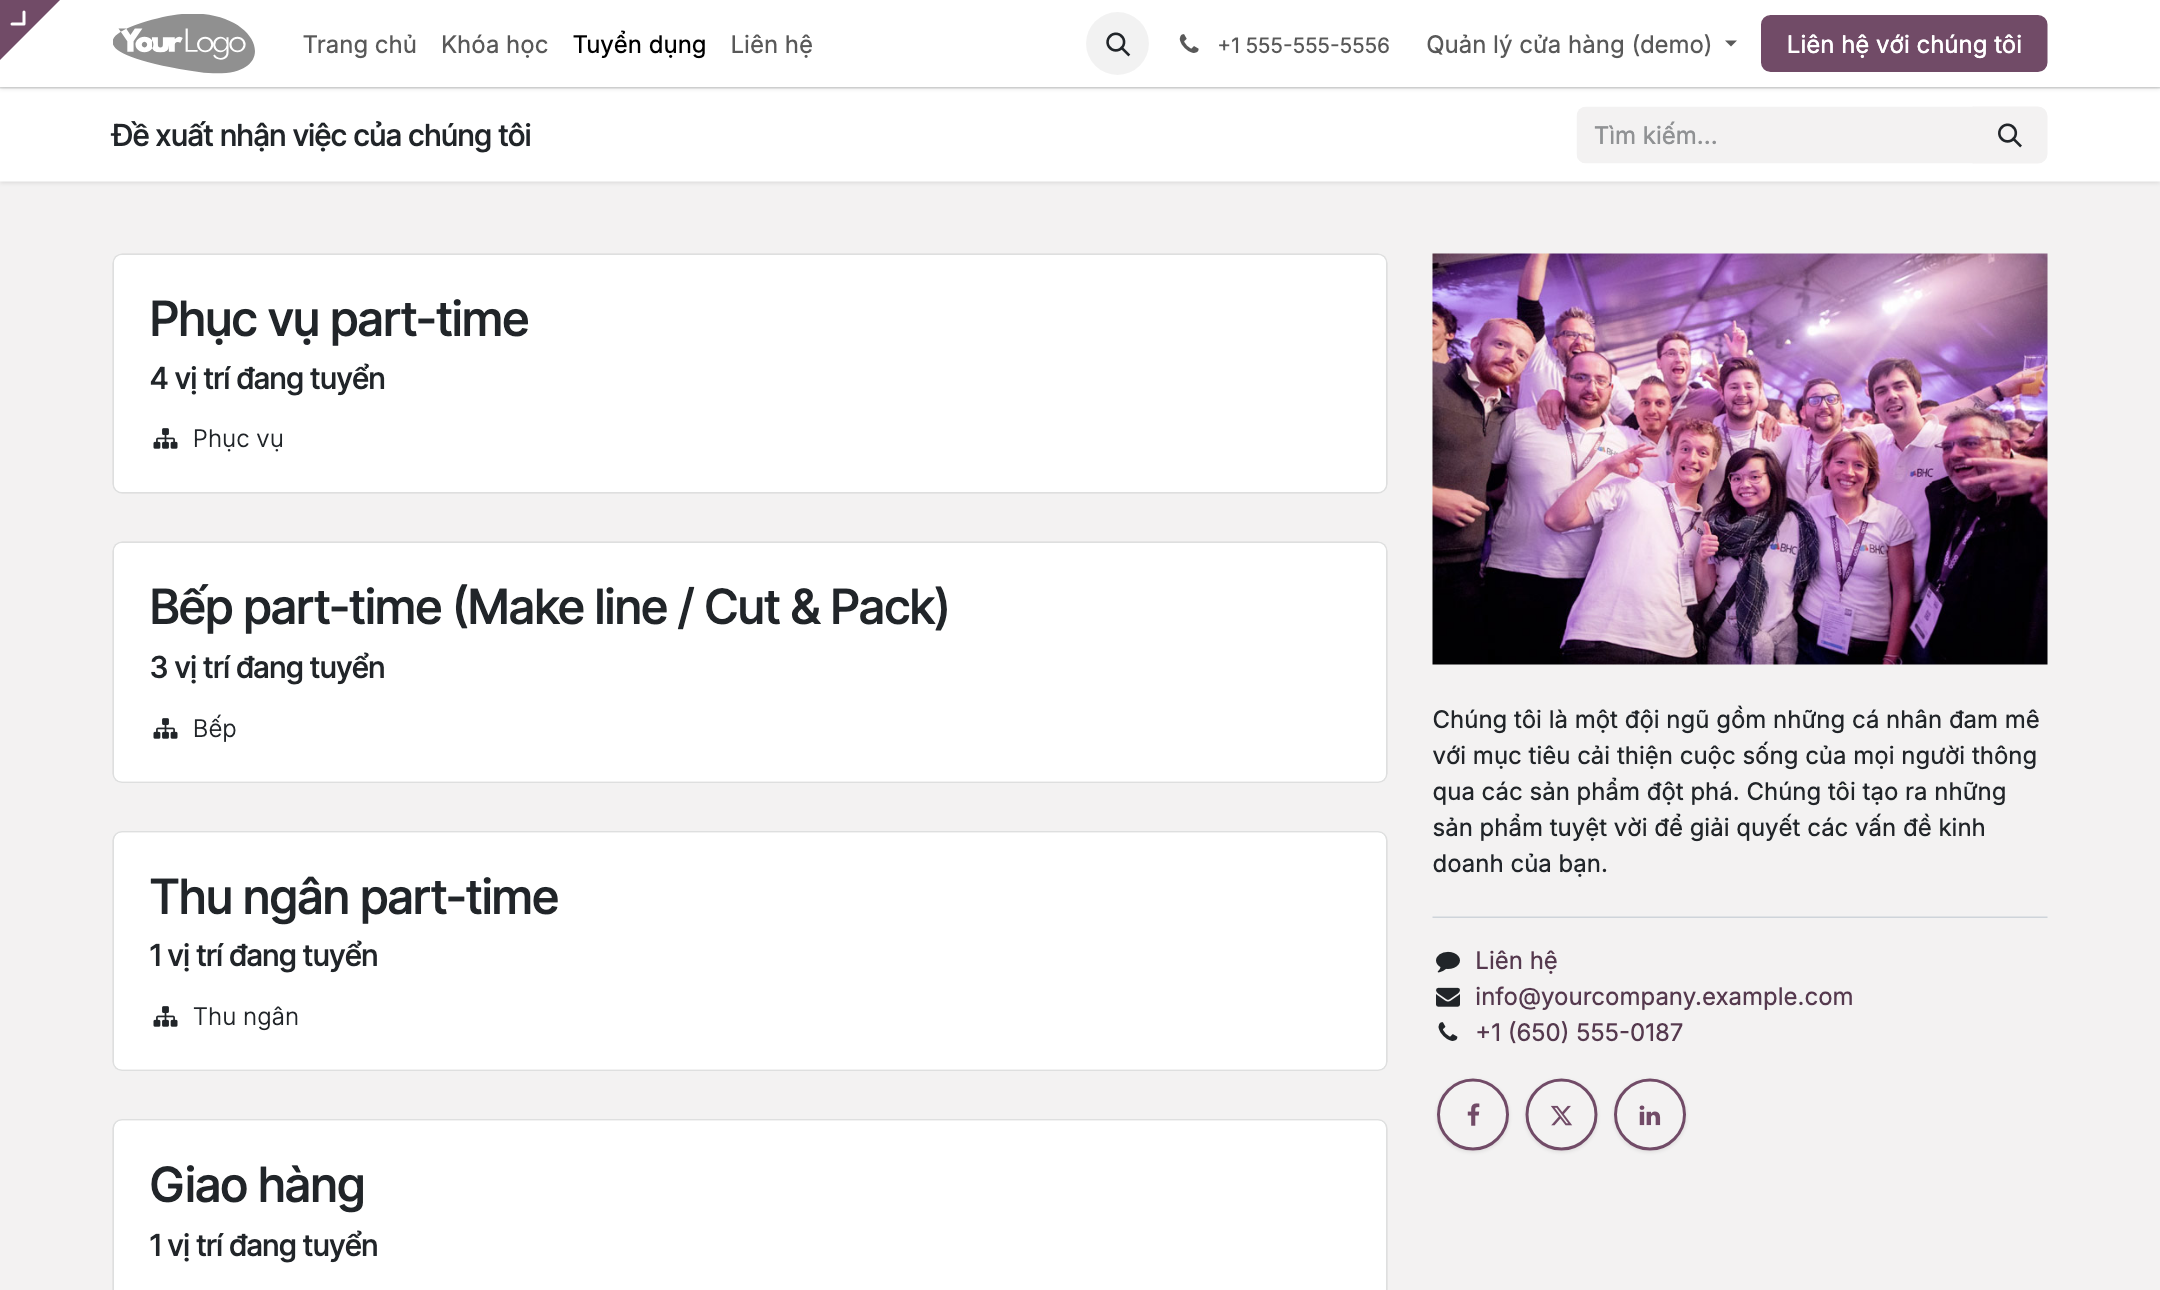
\includegraphics[width=\linewidth]{odoo/jobs_web.png}
\caption{Trang Jobs trên website – ứng viên xem và nộp đơn online}\label{fig:od_web}
\end{figure}
\begin{figure}[H]\centering
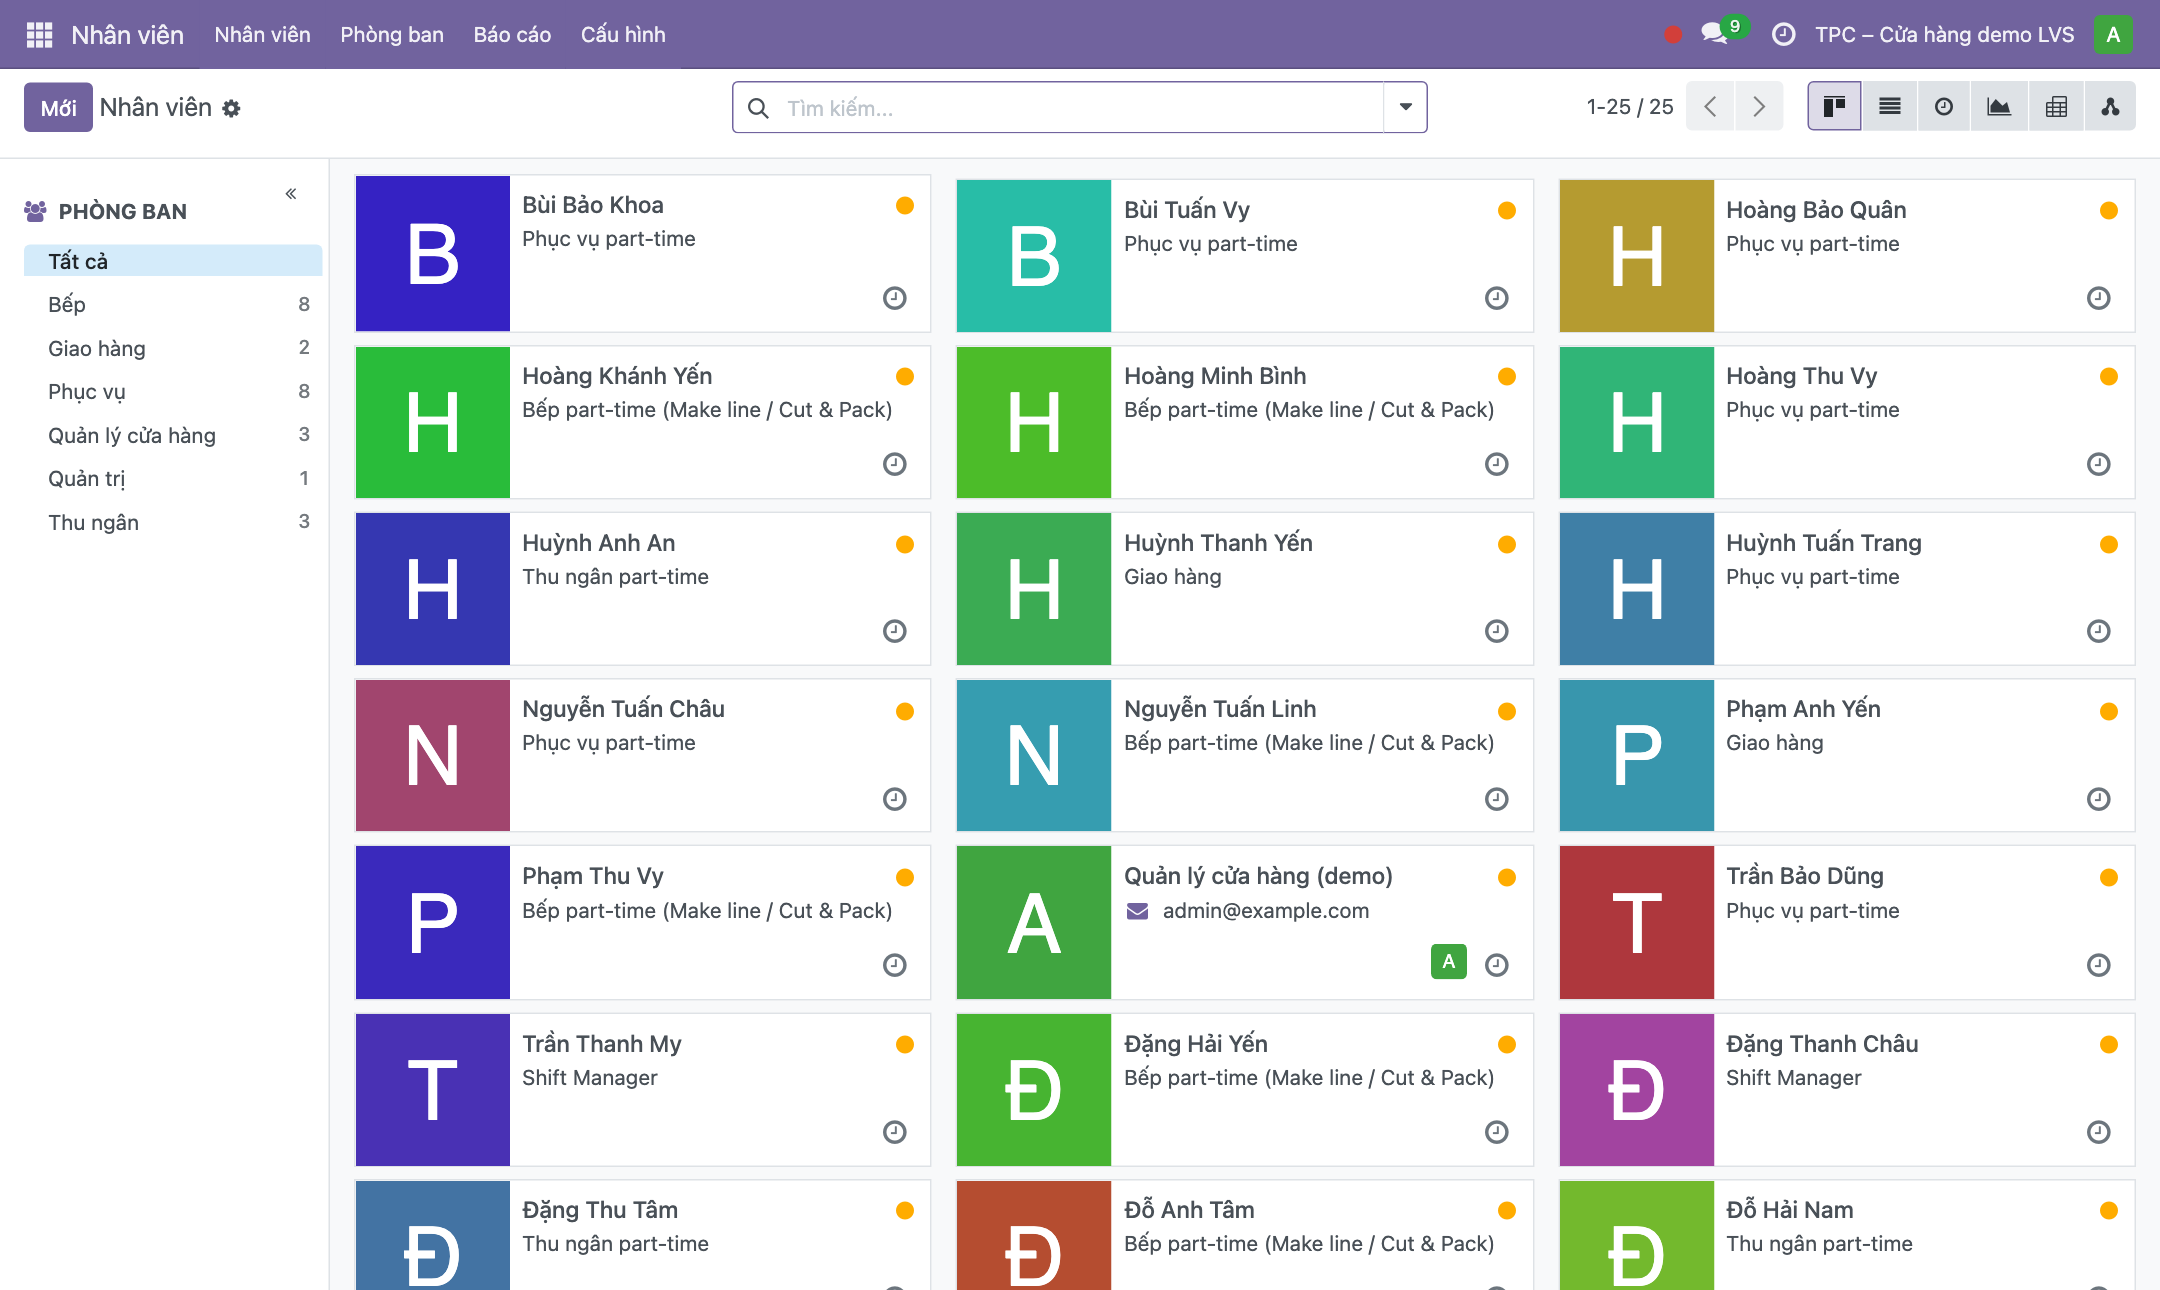
\includegraphics[width=\linewidth]{odoo/employees.png}
\caption{Danh sách nhân viên theo phòng ban (tên giả)}\label{fig:od_emp}
\end{figure}
\begin{figure}[H]\centering
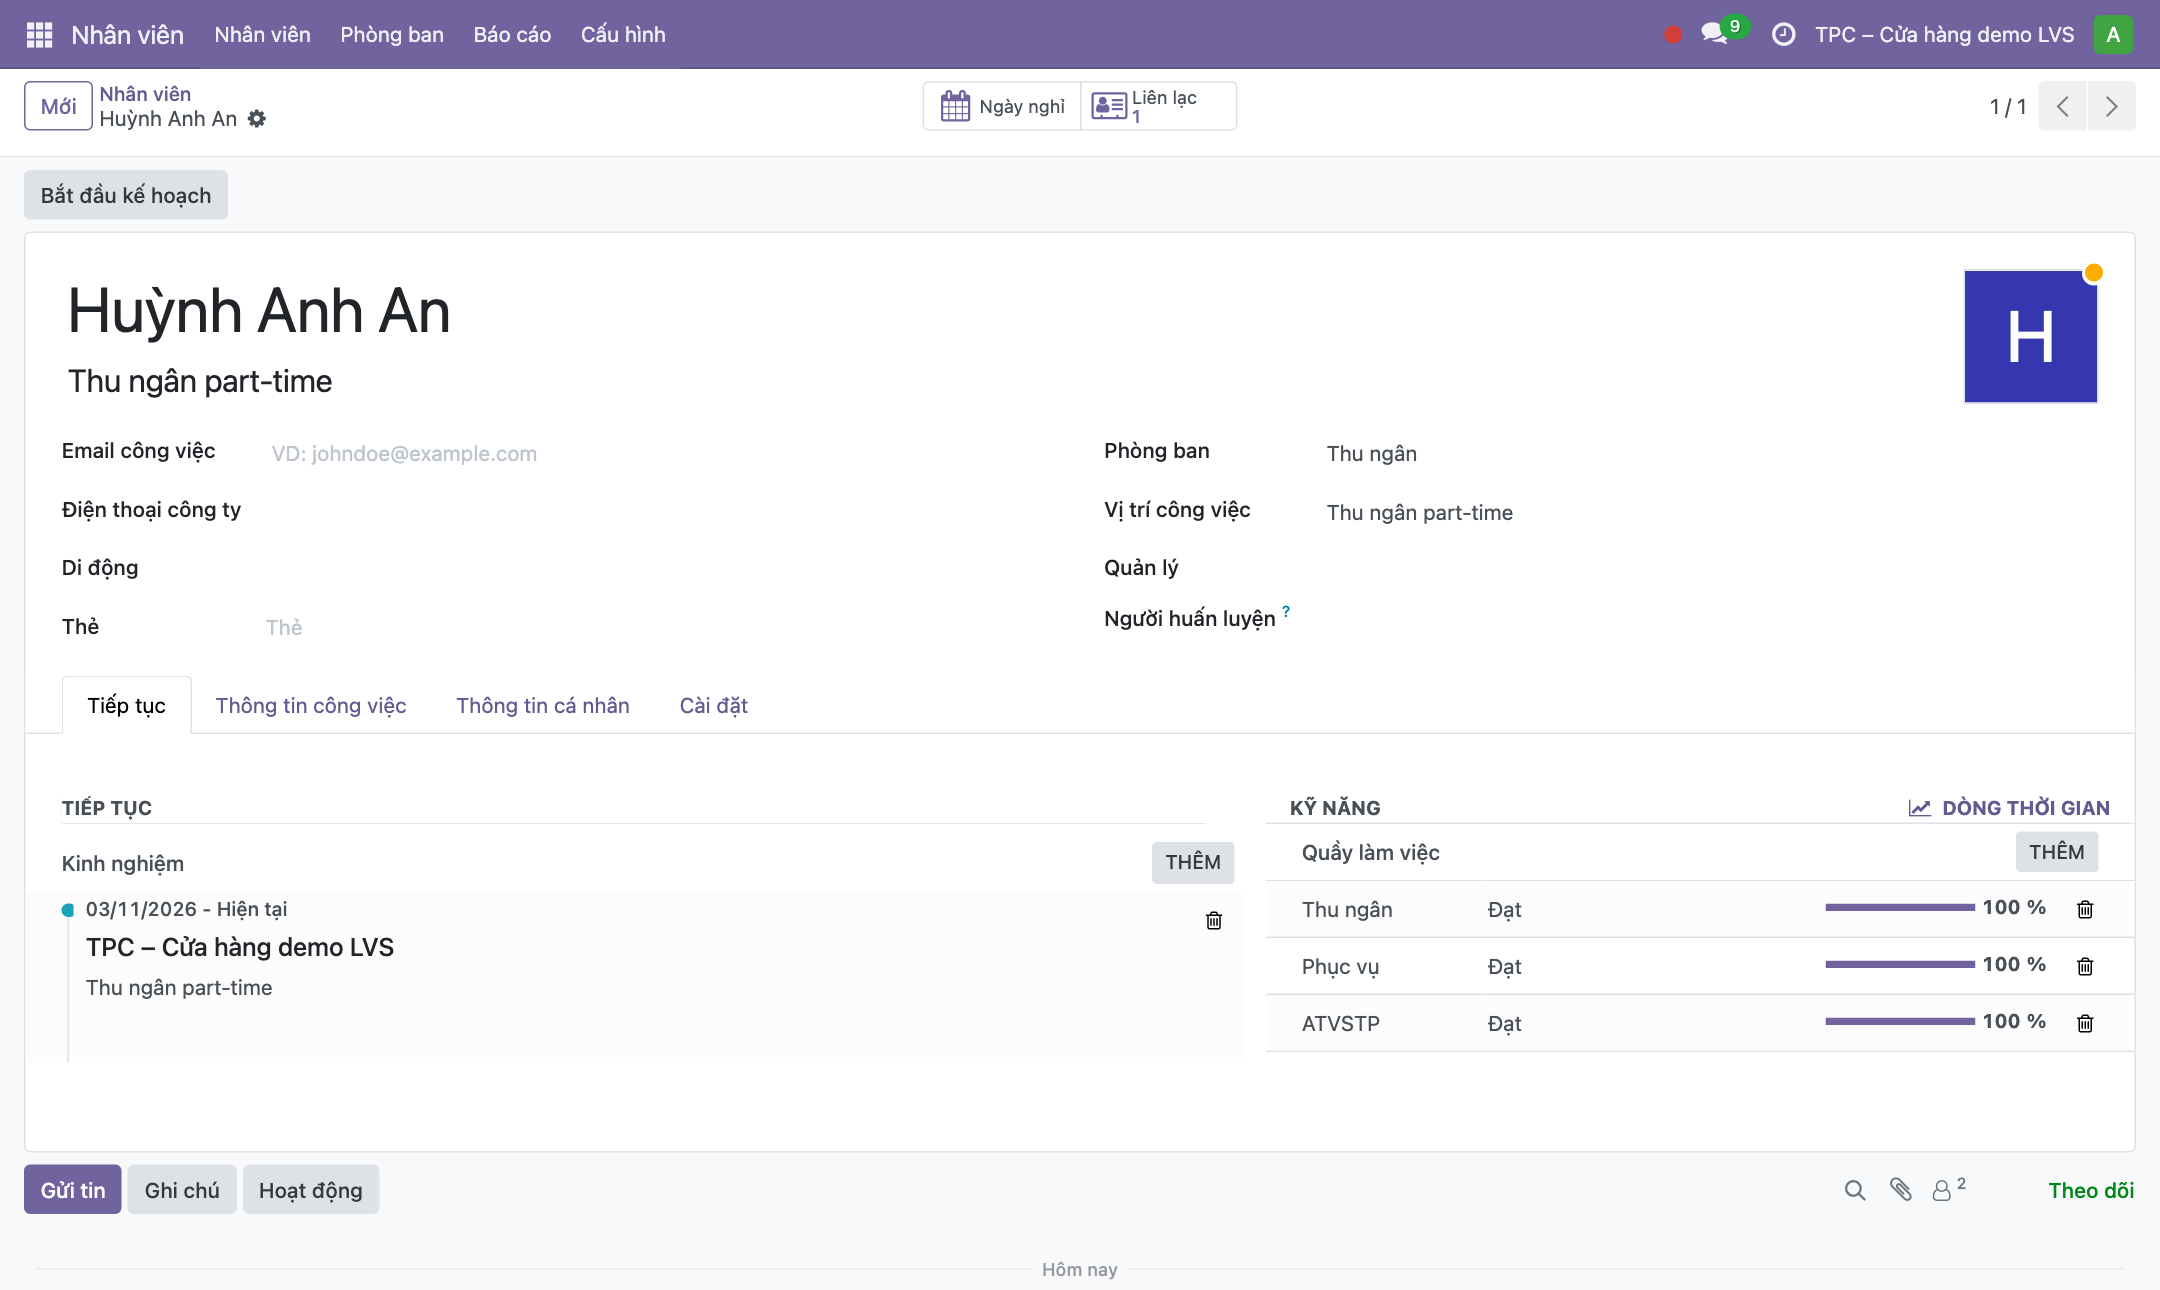
\includegraphics[width=\linewidth]{odoo/emp_form.png}
\caption{Hồ sơ nhân viên với kỹ năng ``Quầy làm việc'' (Đạt/Đang học)}\label{fig:od_empform}
\end{figure}
\begin{figure}[H]\centering
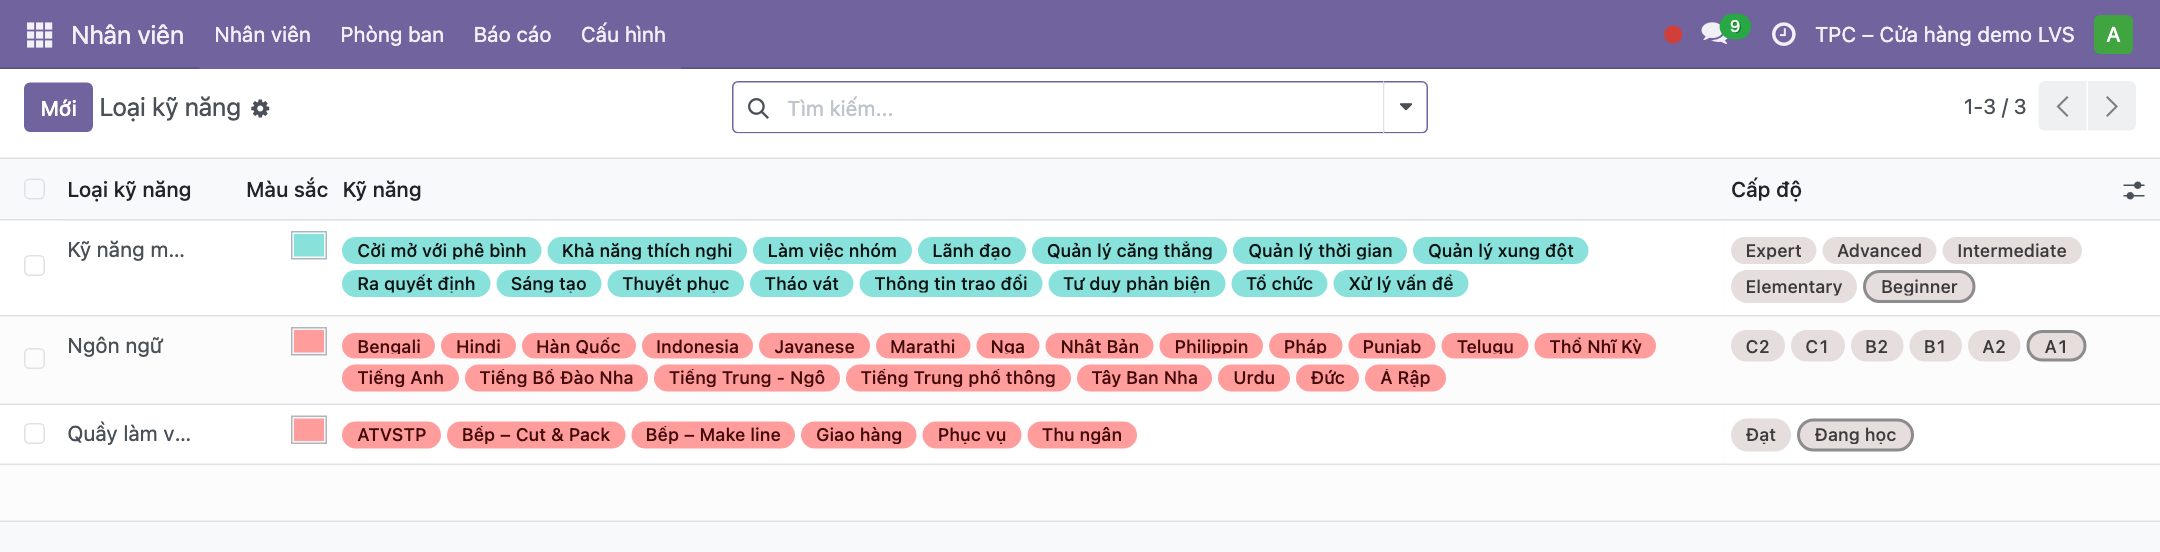
\includegraphics[width=\linewidth]{odoo/skill_types.png}
\caption{Loại kỹ năng ``Quầy làm việc'' và cấp độ}\label{fig:od_skill}
\end{figure}

\section{Đánh giá giai đoạn và kế hoạch tuần 5–6}
\subsection{Đã làm được}
\begin{itemize}
\item Có số liệu định lượng chắc chắn cho vấn đề trung tâm (I4): giờ công thừa ngày vắng, thiếu ngày đông, \%COL vượt mục tiêu 6/8 tháng.
\item Bộ 9 sơ đồ BPMN (1 tổng quát, 4 AS-IS, 4 TO-BE), bảng vấn đề, bảng giá trị, 22 yêu cầu chức năng, use case, 4 đặc tả, sơ đồ lớp, thiết kế vật lý.
\item Odoo 18 chạy ổn định, 10 module HR đã cài và cấu hình đúng quy trình TO-BE.
\end{itemize}
\subsection{Hạn chế và việc cần làm ngay}
\begin{itemize}
\item P3, phần ghi giờ công của P4 đang là giả định → \textbf{phỏng vấn chính thức}, cập nhật sơ đồ lên v2.
\item Chưa có số người tối thiểu mỗi quầy → chưa tính được tiết kiệm thật.
\item Chưa có số liệu nghỉ việc 12 tháng → xin thêm dữ liệu (Phụ lục A, mục 2.2).
\end{itemize}
\subsection{Kế hoạch tuần 5–6}
\begin{itemize}
\item Tuần 5: code add-on MVP (model định mức, Forecast, tính giờ đề xuất, ca, báo cáo ngày); cấu hình eLearning, Survey, Attendances.
\item Tuần 6: báo cáo giữa kỳ (slide và demo MVP); triển khai lên máy chủ có tên miền.
\end{itemize}

% =====================================================================
\begin{thebibliography}{9}
\addcontentsline{toc}{chapter}{Tài liệu tham khảo}
\bibitem{laudon} K. C. Laudon, J. P. Laudon, \emph{Management Information Systems: Managing the Digital Firm}, 16th ed., Pearson, 2020.
\bibitem{dessler} G. Dessler, \emph{Human Resource Management}, 16th ed., Pearson, 2020.
\bibitem{ernst} A. T. Ernst, H. Jiang, M. Krishnamoorthy, D. Sier, ``Staff scheduling and rostering: A review of applications, methods and models'', \emph{European Journal of Operational Research}, vol. 153, no. 1, pp. 3–27, 2004.
\bibitem{bpmn} Object Management Group, \emph{Business Process Model and Notation (BPMN) Version 2.0.2}, 2014.
\bibitem{dumas} M. Dumas, M. La Rosa, J. Mendling, H. A. Reijers, \emph{Fundamentals of Business Process Management}, 2nd ed., Springer, 2018.
\bibitem{odoo} Odoo S.A., \emph{Odoo 18.0 Documentation – Developer \& User Guides}, \url{https://www.odoo.com/documentation/18.0/}.
\bibitem{gv} Tài liệu môn học: ``BPMN – Business Process Model and Notation'' và ``Đồ án HTTTQL'' (slide giảng viên).
\end{thebibliography}

% =====================================================================
\appendix
\titleformat{\chapter}[display]{\bfseries\Large\centering}{PHỤ LỤC \thechapter}{4pt}{\Large\MakeUppercase}
\chapter{Bộ câu hỏi phỏng vấn chính thức}
\emph{Gửi trước cho quản lý ít nhất 3 ngày. Xin phép ghi âm ở đầu buổi.}

\textbf{A. Tuyển dụng}
\begin{enumerate}
\item Mỗi tháng cửa hàng tuyển trung bình bao nhiêu người? Bao nhiêu người đến phỏng vấn, bao nhiêu người được nhận?
\item Tính từ lúc ứng viên hỏi việc đến khi có mã NV và đi làm ca đầu tiên mất bao nhiêu ngày? Bước nào chậm nhất?
\item Ứng viên đến từ nguồn nào (standee, fanpage, phòng tuyển dụng gửi data, người quen)? Nguồn nào hiệu quả nhất?
\item Có khi nào bị sót ứng viên, quên hẹn, hoặc ứng viên đã hẹn mà không đến không?
\item Thông tin ứng viên đang lưu ở đâu: giấy, link form hay Excel?
\end{enumerate}
\textbf{B. Onboarding và đào tạo}
\begin{enumerate}[resume]
\item Training plan 2 tuần gồm những gì? Có thể cho nhóm xem bản mẫu (đã che thông tin nội bộ) không?
\item Bài test cuối đào tạo chấm thế nào, ai chấm, kết quả lưu ở đâu?
\item Khoảng bao nhiêu phần trăm nhân viên mới nghỉ trong 2 tuần hoặc 1 tháng đầu?
\item Cửa hàng có bao nhiêu quầy? Một người có làm được nhiều quầy không?
\end{enumerate}
\textbf{C. Xếp ca và chấm công}
\begin{enumerate}[resume]
\item Ai xếp ca? Xếp bằng gì (Excel, giấy, Zalo)? Xếp trước bao lâu?
\item Khi xếp ca có nhìn vào Forecast Sales không? Định mức 330.000 đ/giờ được dùng thế nào?
\item \textbf{Mỗi ca, mỗi quầy tối thiểu cần mấy người?}
\item Đổi ca hoặc nghỉ đột xuất xử lý thế nào? Thường báo trước bao lâu?
\item Chấm công bằng gì? Giờ thực tế (Actual WH) được ghi vào file Store Performance lúc nào, ai ghi? Ngày lễ có nhân hệ số không?
\end{enumerate}
\textbf{D. Nghỉ việc}
\begin{enumerate}[resume]
\item Tỷ lệ nghỉ việc theo tháng (nhất là tháng 2)? Có số liệu 12 tháng không?
\item Lý do nghỉ chủ yếu? Có phỏng vấn trước khi nghỉ không?
\end{enumerate}
\textbf{E. Mong muốn}
\begin{enumerate}[resume]
\item Nếu có hệ thống tự gợi ý số giờ ca theo dự báo doanh thu, chú có dùng không? Cần hiện những gì?
\end{enumerate}

\textbf{Dữ liệu, biểu mẫu xin thêm}: bảng xếp ca mẫu 1–2 tuần (che tên); training plan hoặc checklist theo quầy; mẫu tin tuyển dụng, mẫu đơn ứng tuyển; số người nghỉ việc và tuyển mới theo tháng; danh sách quầy và số người tối thiểu.

\chapter{Phiếu khảo sát (Google Form)}
\emph{Đối tượng: quản lý ca, nhân viên part-time (3–5 người/cửa hàng). Ẩn danh.}
\begin{enumerate}
\item Vai trò của bạn: \quad $\square$ Quản lý ca \quad $\square$ Nhân viên part-time \quad $\square$ Nhân viên full-time
\item Bạn làm ở cửa hàng được bao lâu? \quad $\square$ < 1 tháng \quad $\square$ 1–6 tháng \quad $\square$ 6–12 tháng \quad $\square$ > 1 năm
\item (Quản lý ca) Mỗi tuần bạn mất bao nhiêu phút để xếp ca? \quad \underline{\hspace{2cm}}
\item Lịch ca được gửi qua kênh nào? \quad $\square$ Zalo \quad $\square$ Giấy dán \quad $\square$ Excel/email \quad $\square$ Khác
\item Bạn nhận lịch ca trước ca đầu tiên của tuần bao nhiêu ngày? \quad \underline{\hspace{2cm}}
\item Tháng vừa rồi bạn đổi ca hoặc nhờ người thay bao nhiêu lần? \quad \underline{\hspace{2cm}}
\item Có ca nào bạn thấy \emph{quá đông người} so với lượng khách không? \quad $\square$ Thường xuyên \quad $\square$ Thỉnh thoảng \quad $\square$ Hiếm khi
\item Có ca nào bạn thấy \emph{thiếu người} không? Thường vào ngày nào? \quad \underline{\hspace{3cm}}
\item Từ lúc phỏng vấn đến ca làm đầu tiên của bạn mất bao nhiêu ngày? \quad \underline{\hspace{2cm}}
\item Bạn mất bao lâu để làm được quầy đầu tiên một mình? \quad \underline{\hspace{2cm}}
\item Bạn có muốn xem lịch ca, xin đổi ca, học bài trên điện thoại không? (1–5)
\item Góp ý khác: \underline{\hspace{8cm}}
\end{enumerate}

\chapter{Mẫu biên bản phỏng vấn}
\begin{tabularx}{\linewidth}{|L{4cm}|Y|}
\hline Thời gian, địa điểm & \\\hline
Người được phỏng vấn (chức vụ) & \\\hline
Thành viên nhóm tham gia & \\\hline
Hình thức ghi nhận & $\square$ Ghi âm \quad $\square$ Quay video \quad (đã xin phép: $\square$) \\\hline
Nội dung chính theo nhóm câu hỏi A–E & \\[2.5cm]\hline
Số liệu, biểu mẫu nhận được & \\\hline
Điểm cần xác nhận lại & \\\hline
Xác nhận của người được phỏng vấn & \\[1.2cm]\hline
\end{tabularx}

\chapter{Minh chứng quá trình làm việc}
\begin{itemize}
\item \textbf{Mã nguồn hình vẽ}: tất cả sơ đồ BPMN, UML, biểu đồ trong báo cáo được sinh từ script Python trong thư mục \texttt{scripts/} (\texttt{bpmn.py} là thư viện vẽ BPMN nhóm tự viết; \texttt{fig\_p1.py} … \texttt{fig\_p4.py}, \texttt{fig\_uml.py}, \texttt{charts.py}). Chạy lại script sẽ ra đúng hình, có thể theo dõi phiên bản trên GitHub.
\item \textbf{Môi trường Odoo}: \texttt{odoo/docker-compose.yml}, \texttt{odoo/scripts/setup\_db.py}, \texttt{configure\_hr.py}, \texttt{screenshots.py}.
\item \textbf{Biên bản họp nhóm hằng tuần}: \todo{nhóm bổ sung: ngày, người tham gia, việc đã làm, việc tuần sau}.
\item \textbf{File ghi âm phỏng vấn} và bản gỡ băng: \todo{đường dẫn Drive}.
\item \textbf{Phạm vi sử dụng công cụ AI}: \todo{nhóm ghi rõ phần nào có dùng AI hỗ trợ (VD: gợi ý code vẽ hình, soát chính tả) và phần nào nhóm tự thực hiện}.
\end{itemize}

\end{document}
